\documentclass[m,intern,palatino]{cgBA}


\usepackage{hyperref}						% Verlinkung von Textstellen
\usepackage{fancyhdr}						% eigener Satzspiegel
\usepackage{hypcap} 						% korrekte Verlinkung von Bildern o..
\usepackage{color}						% Einbindung von Farbe
\usepackage{alltt}						% Umschaltung auf typewriter, z.B. fr Quellcode
\usepackage{enumerate}						% Anpassung nummerierter Listen durch optionalen Parameter


\usepackage{mathtools}
\usepackage{empheq}
\usepackage{fancybox}
\usepackage{fancyvrb}


\usepackage{amsfonts}						%
\usepackage{amssymb}						%	Mathe-Zeugs
\usepackage{amsmath}						%

\usepackage{moreverb}						% Erweiterung der verbatim-Umgebung (zum Einbinden von Code)
\usepackage{array}
\usepackage{url}
\usepackage{tabularx}

\usepackage[disable]{todonotes}


%-----------------------------------------------------------------------------------------------------------


\setcounter{secnumdepth}{7} 	%seven levels of nesting
\setcounter{tocdepth}{7}%
\usepackage{subsections} 	%some definitions for subsubsubsections etc..



\graphicspath{{pictures/}}

%-----------------------------------------------------------------------------------------------------------

\begin{document}

\author{Markus Schl{\"u}ter}
\title{Konzeption und Implementierung eines Unified Rendering Frameworks mit modernen GPU-Computing-APIs}
\zweitgutachter{Dipl.-Inform.  Dominik Gr{\"u}ntjens}




% Umschalten der Sprache (für englische Rubrikbezeichnungen etc.)
%\selectlanguage{english}


%-----------------------------------------------------------------------------------------------


\maketitle
\clearpage 


\pagenumbering{roman}


\listoftodos		%TODO list, the most important thing in any document ;)
\tableofcontents
\clearpage         	% oder \cleardoublepage bei zweiseitigem Druck
% \listoffigures   % fuer ein eventuelles Abbildungsverzeichnis
% \clearpage

\pagenumbering{arabic}


% Hier kommt jetzt der eigentliche Text der Arbeit

\section{Einleitung}
	

Im Rahmen dieser Bachelorarbeit wurde der Frage nachgegangen, inwiefern eine sogenannte "`Unified Rendering-Engine", welche verschiedene Simulationsdomänen vereint, einen Mehrwert darstellen kann gegenüber dem klassischen Ansatz, z.B. gesondert sowohl eine Graphik- als auch eine Physik-Engine zu verwenden, die zunächst einmal keinen
Bezug zueinander haben;\\

Hierbei wurde besonderer Wert auf die Verwendung moderner GPU-Computing-APIs gelegt, namentlich auf OpenGL3/4 und OpenCL.\\
Da bei diesem ganzheitlichen Thema eine vollständige Implementierung einer solchen vereinheitlichten Engine unmöglich war,
konnte nur ein Bruchteil der Konzepte implementiert werden;\\

Dieser Umstand war von Vornherein bekannt, und die Versuchung ist stark, wie in einer Demo die schnelle Realisierung eines Feature-Sets einer konsistenteren, aber zeitaufwändigeren und zunächst karger wirkenden Implementierung vorzuziehen.
Dieser Versuchung wurde versucht, nur dort nachzugeben, wo die negativen Auswirkung auf die Konsistenz des Gesamtsystems lokal bleiben, und so nicht "`Hacks"' sich irreversibel durch das gesamte System ziehen.\\

Letztendlich wurden exemplarisch für die Nutzung in  der visuellen Simulationsdomäne einige gängige visuelle Effekte einer Graphik-Engine implementiert, wie  Shadow Mapping, Normal Mapping, Environment Mapping, Displacement Mapping und dynamisches LOD. Es wurden moderne OpenGL- und Hardware-Features wie Instancing, Uniform Buffers und Hardware-Tesselation verwendet. Schwerpunkt war hier der Einsatz einer Template-Engine, damit
\begin{enumerate}
	\item Boilerplate-Code in den Shadern vermieden wird und
	\item Effekte beliebig (sinnvoll) nach Möglichkeit zur Laufzeit miteinander kombinierbar sind
\end{enumerate}
. Mehr dazu in Kapitel \ref{sec:visualDomain}\\
In der mechanischen Simulationsdomäne wurde eine partikelbasierte Fluidsimulation mit OpenCL auf Basis von Smoothed Particle Hydrodynamics implementiert. Mehr dazu in Kapitel \ref{sec:mechanicalDomain}.\\

Das System trägt den Namen "`Flewnit"', eine bewusst nicht auf den ersten Blick erkennbar sein sollende\footnote{Es soll der generalistische Ansatz des Frameworks nicht in den Hintergrund gedrängt werden.} Kombination der Worte "`Fluid"', in Anspielung auf den urspünglichen Zweck einer Bibliothek zur Fluidsimulation und "`Unit"', in Anspielung auf "`Unity"'-"`Einheit"'. Zufälligerweise ist das $Nit$ auch noch die englische Einheit für die Leuchtdichte, $Cd \over m^2$.


\subsection{Motivation}

Ursprünglich als Arbeit zur Implementierung einer Fluidsimulation geplant, wurde bald ein generalistischer, eher softwaretechnisch orientierter Ansatz verfolgt, der jedoch die Implementierung einer Fluidsimulation mittelfristiges Ziel hatte;\\

\subsubsection{"`Unified Rendering Engine"'}
Der Wunsch nach einer "`Unified Rendering Engine" erwächst aus eigener Erfahrung der Kopplung von Physik- und Graphik-Engines, namentlich der Bullet Physics Library\footnote{http://bulletphysics.org} und der OGRE Graphik-Engine\footnote{http://www.ogre3d.org}. Diese Hochzeit zweier Engines, die jeweils für verschiedene "`Simulationsdomänen"' zuständig sind, bringt gewissen Overhead mit sich, da Konzepten wie  Geometrie und ihrer Transformationen unterschiedliche Repräsentationen bzw. Klassen zugrunde liegen;
Hierdurch wird die gemeinsame Nutzung beider Domänen von Daten wie z.B. Geometrie nahezu unmöglich; Ferner müssen für eine die beiden Engines benutzende Anwendung diese Klassen mit ähnlicher Semantik durch neue Adapterklassen gewrappt werden,
um dem Programmier der eigentlichen Anwendungslogik den ständigen Umgang mit verschiedenen Repräsentationen und deren Synchronisation zu ersparen.\\

\todo{evtl. beispielschema erstellen für zwei klassischee transformationsklassen und adapter vs. unified transformation}

Die Aussage "`Photorealistische Computergraphik ist die Simulation von Licht"' \todo{Zitat einfügen? Stefan Müller, PCG? ;)} hat mich wohl auch inspiriert, den Simulationsbegriff allgemeiner aufzufassen und das Begriffspaar "Rendering und Physiksimulation"' zu hinterfragen\footnote{Auch wenn dieses Framework nicht vornehmlich auf physikalisch basierte, also photorealistische Beleuchtung ausgelegt ist, soll diese aufgrund des generalistischen Konzepts jedoch integrierbar sein.}.

Es sei bemerkt, dass weder eine Hypothese bestätigt noch widerlegt werden sollte, geschweige denn überhaupt eine (mir bekannte) Hypothese im Vorfeld existierte; Es sprechen etliche Argumente für eine Vereinheitlichung der Konzepte (geringerer Overhead durch Wegfall der Adapterklassen, evtl. Speicherverbrauch durch z.T. gemeinsame Nutzbarkeit von Daten), aber auch einige dagegen (Komplexität eines Systems, Anzahl an theoretischen Kombinationsmöglichkeiten steigt, viele sind unsinnig und müssen implizit oder explizit ausgeschlossen werden).\\

Für mich persönlich bringt die Bearbeitung dieser Fragestellung zahlreiche Vorteile; Ich muss ein wenig ausholen:\\
Schon als Kind war ich begeistert von technischen Geräten, auf denen interaktive Computergraphik möglich war; Sie sprechen sowohl das ästhetische Empfinden an, als auch bieten sie eine immer mächtigere Ergänzungs- und  Erweiterungsmöglichkeit zu unserer Realität an; Letztendlich stellten diese Geräte für mich wohl auch immer ein Symbol dafür dar, in wie weit die Menschheit inzwischen fähig ist, den Mikrokosmos zu verstehen und zu nutzen, damit demonstriert, dass sie zumindest die rezeptiven und motorischen Beschränkungen seiner Physiologie überwunden hat.\\
Die Freude an Schönheit und Technologie findet für mich in der Computergraphik und der sie ermöglichenden Hardware eine Verbindungsmöglichkeit; Die informatische Seite mit seinen Algorithmen als auch die technische Seite mit seinen Schaltungen faszinieren mich gleichermaßen; Auch das "`große Ganze" der Realisierung solcher Computergraphischen Systeme, das Engine-Design mit seinen softwaretechnischen Aspekten, interessiert mich.\\
Ferner wollte ich schon immer "die Welt verstehen", sowohl auf physikalisch-naturwissenschaftlich-technischer, als auch - aufgrund der system-immanenten Beschränkungen unseres Universums - auf metaphysischer Ebene\footnote{ob der Begriff "`Verständnis"' im letzten Falle ganz treffend ist, bleibt Ermessens-Sache};\\

Und hier schließt sich der Kreis: Sowohl in der Philosophie als auch in der Informatik spielt das Konzept der Abstraktion eine wichtige Rolle; Nichts anderes tut eine "`Unified Engine": sie abstrahiert bestehende Konzepte teilgebiets-spezifischer Engines, wie z.B. Graphik und Physik; Ich erhoffe mir, dass mit dieser Abstraktion man in seinem konzeptionellen Denken der der realen Welt ein Stück weit näher kommt; Die verfügbaren Rechenressourcen steigen, die Komplexität von Simulationen ebenfalls; Ob eine semantische Generalisierung von seit Jahrzehnten verwendeten Begriffen wie "`Rendering"' und "`Physiksimulation"', welche dieser Entwicklung angemessen sein soll, eher hilfreich oder verwirrend ist, kann eine weitere Interessante Frage sein, die ich jedoch nicht weiter empirisch untersucht habe.\\

Letzendlich verbindet dieses Thema also viele meiner Interessen, welche die gesamte Pipeline eines Virtual-Reality-Systems,  vom Konzept einer Engine bis hin zu den Transistoren einer Graphikkarte, auf sämtlichen Abstraktionsstufen betreffen: Es gab mir die Möglichkeit,
\begin{itemize}
	\item den Mehrwert einer Abstraktion gängiger Konzepte von Computergraphik und Physiksimulation zu erforschen
	\item meine Erfahrung im Engine-Design zu vertiefen
	\item meine Erfahrungen im (graphischen) Echtzeit-Rendering zu vertiefen
	\item mich mit Physiksimulation (genauer: Simulation von Mechanik) zu beschäftigen, konkret mit Fluidsimulation
	
	\item mich in OpenGL 3 und 4 einzuarbeiten, drastisch entschlackten Versionen der Graphik-API, deren gesäuberte Struktur die Graphikprogrammierung wesentlich generalistischer macht und somit die Abstraktion erleichtert
	\item mich in OpenCL einzuarbeiten, den ersten offenen Standard für \linebreak GPGPU\footnote{General Purpose Graphics Processing Unit- Computing, die Nutzung der auf massiver Paralleltät beruhenden Rechenleistung von Graphikkarten in nicht explizit Graphik-relevanten Kontexten}
	\item  mich intensiver mit Graphikkarten-Hardware, der zu Zeit komplexesten und leistungsfähigsten Consumer-Hardware zu beschäftigen, aus purem Interesse und um die OpenCL-Implementierung effizienter zu gestalten

\end{itemize}

\subsubsection{Fluidsimulation}
Warum Fluid?
 interesse an physik, "seichter einstieg" durch verinfachte Algorithmen, so lange es "nur" um plausibilität geht und nicht um physikalische korrektheit, einfacheres Mapping der homogh
Warum Partikelbasiert?
... theoretisch unendliche simulationsdomäne, direkte darstellungsmöglichkeit als openGL vertices, damit directe nutzung von CL/GL interop und somit gemeinsamer nutzung von daten ind beiden domänen..., einfachere mathematik dank lagrange'scher betrachtung, kein advektionsterm, besser einsetzbar für Liquide, da Voxelbasierte ansätze "tricksen" müssen, um das volumen einer teilmenge eines Fluids zu bbewahren;

\clearpage

	
\section{Überblick}
	
\subsection{Vision}

Die langfristige Vision, die \emph{Flewnit} begleitet, ist die Entwicklung eines interaktiven Paddel-Spiels unter Verwendung dieser Unified Engine mit ausgefeilter Fluid-Mechanik und -Visualisierung, partikelbasierten Rigid Bodies und Dreiecks-Mesh als Repräsentation für statische Kollisions-Geometrie; Spiele, in der große Mengen Fluid, die komplexer simuliert sind als durch Height-Fields
\footnote{s. Kapitel \ref{sec:relatedWork} für mehr Informationen zu Height-Field-basierter Fluidsimulation}
einen integrativen Bestandteil der Spielmechanik ausmachen, sind mir nicht bekannt;\\
Von Dreiecks-Geoemetrie erhoffe ich mir eine genauere Repräsentation zur Kollisionsbehandlung, bei gleichzeitiger Ersparnis vieler Partikel, die sonst z.T große Oberflächen repäsentieren müssten; Ferner könnte die Dreiecksstruktur später zur Simulation nicht-partikelbasierter Rigid Bodies verwendet werden;


\subsection{Paradigmen}
\label{sec:paradigm}

Vor dem Entwurf eines komplexen Softwaresystems mit einigen Zügen, die in etablierten Systemen keine so große Bedeutung haben, hat es Sinn, sich einige Paradigmen zu überlegen, welchen das System nach Möglichkeit folgen soll, um eine gewisse Konsitenz zu gewährleisten:
	
\begin{itemize}
	\item Es wurde beim Entwurf der Unified Engine für jede Simulationsdomäne eine möglichst ähnliche Struktur von Klassen 	
	und ihren Beziehungen zueinander angestrebt. Diese Ähnlichkeit spiegelt sich nach Möglichkeit in einer gemeinsamen 	
	(manchmal abstrakten) Oberklasse eines jeden Konzeptes wider, wie z.B.:
	\begin{itemize}
		\item dem Simulations-Objekt als solchem
		\item der Geometrie
		\item dem Material
		\item der Szenen-Repräsentation
	\end{itemize}
	Auf diese Weise soll eine maximale \emph{Symmetrie} zwischen den Domänen hergestellt werden, so dass domänen-bedingte 
	Spezial-Behandlung von Objekten und Workflows minimiert wird;

	\item Es sollte eine Art Pipeline-Architektur entstehen, wo bestimmte Pipeline-Stages bestimmte Simulations-(Zwischen)-
	Ergebnisse implemetieren, und ggfs. anderen Stages diese zur Verfügung stellen. Jede Simulationsdomäne hat seine eigene 
	Pipeline; Dennoch können Interdependenzen bestehen;\\
	Diesen Interdependenzen wird durch eine Konzept-spezifische Verwaltung durch verschiedene Singleton-Manager-Klassen 	
	genüge getan; Ein und dasselbe Objekt kann von verschiedenen Managern in unterschiedlichem Zusammenhang verwaltet 
	werden; Mehr dazu in Kapitel \ref{sec:systemArchitecture};

	\item Es sollen langfristig so viele Features (Visualisierungstechniken und -effekte, Simulationstechniken) wie möglich 
	miteinander kombinierbar sein, sofern die Kombination nicht unsinnig ist;

	\item Es soll so viel wie möglich auf der GPU berechnet werden, um die massive Paralleltät auszunutzen, 
	und um nicht durch Buffer-Transfers, die die Aufteilung von Algorithmen in CPU- und GPU- Code meist mit sich bringen, 	
	auf den Bandbreiten- und Latenz- Flaschenhals der PCI-Express-Schnittstelle zu stoßen;
	\todo{hier specs und refs zu PCIe 2.0 anbringen? eher nicht, oder?}
	
	\item Es soll immer das Potential gewahrt werden, dass aus dem Framework --- außerhalb des Rahmens dieser 
	Bachelorarbeit --- tatsächlich noch eine Art \emph{Unified Engine} entstehen kann; Somit sind "`schnelle Hacks"',
	also unsaubere Programmier-Weisen, die mit geringstem Programmier-Aufwand ein bestimmtes Feature implementieren,
	überall dort unbedingt zu vermeiden, wo sie die konsistente Gesamstruktur des Systems zu bedrohen scheinen.

\end{itemize}



	


\subsection{Begriffe}

Im Zuge der angestrebten Vereinheitlichung der  verschiedenen Simulation müssen wir auch einige Begriffe verallgemeinern, 
welche in ihrer jahrzentelangen Tradition in der Terminologie der Computergraphik eine spezifische Bedeutung erhalten haben;
Zur besserern Einordnung stellt Abbildung \ref{fig:classicalVsUnified} ein grobes Schema dar, welches die klassische Verwendung verschiedener Engines und die einer Unified Engine gegenüber stellt:



	\begin{figure}[ht]
		%\centering
		\def\svgwidth{\textwidth}
	    \input{classicalVsUnified.pdf_tex}
	   	%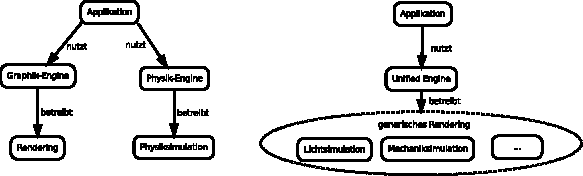
\includegraphics[width=\textwidth]{classicalVsUnified.pdf}
		\caption{Gegenüberstellung von Verwendung und Begrifflichkeiten von klassischen Engines und einer Unified Engine}
		\label{fig:classicalVsUnified}
	\end{figure}
	




\begin{description}

	\item[Rendering]
	Im Wiktionary \cite{internet:wiktionRender} wird das Verb \emph{to render} u.a. umschrieben als:
	\begin{quote}
		"`(transitive, computer graphics) To transform digital information in the form received from a repository into a 
		display on a computer screen, or for other presentation to the user. "'
	\end{quote}	
	Es geht also um die Transformation einer formalen Beschreibung in eine für einen menschlichen Benutzer wahrnehmbare 
	Form. Diese muss entgegen der gewöhnlichen Verwendung des Begriffes nicht zwingend visuell, sondern kann z.B. auch 
	akustischer oder haptischer Natur sein, übertragen durch Lautsprecher oder Force-Feedback-Devices.\\
	
	Verallgemeinern wir den Begriff \emph{Rendering} weiter, gemäß der Übersetzung der Verb-Form als 
	\emph{erbringen}, \emph{machen} \cite{internet:dictCCrender},	
	und in Anlehnung an seine Ethymologie,
	\begin{quote}
		"`From Old French \emph{rendre} (“to render, to make”)"' [...] \cite{internet:wiktionRender}
	\end{quote}
	
	bietet sich eine freie Übersetzung als \emph{Erzeugung eines Zustandes beliebiger Natur} an;\\
	Unter diese generische (Um)-Deutung des Begriffes fällt nun auch \emph{die Ausführung beliebig gearteter Simulation}.
	
	Zu besseren Abgrenzung kann man von \emph{generischen Rendering} und dem klassischen 
	\emph{visuellen Rendering} sprechen; Dies soll im weiteren Verlauf dieser Arbeit der Fall sein.\\
	Eine \emph{Unified Engine} (s.u.) betreibt also \emph{generisches Rendering}.
	
	
	\item[Unified Engine] Alternativ-Bezeichnung: \emph{Unified Rendering Engine};\\
	Eine \emph{Unified Engine} betreibt \emph{generisches Rendering}, indem sie bestimmte Aspekte einer 
	\emph{Welt}\footnote{Diese Welt muss dabei nicht zwingend unserer Realität ähneln oder entsprechen.} simuliert. 
	Darunter kann das klassische (visuelle) Rendering fallen, aber auch die Simulation von Geräuschen und von Mechanik, und 
	beliebige weitere Domänen; Die Domänen sollen dabei durch Abstraktion gemeinsamer Eigenschaften so ähnlich wie möglich
	organisiert sein;
	
	\item[Simulation] Das Begriffspaar \emph{Rendering} und \emph{Physiksimulation} ist im Kontext dieser versuchten 
	Vereinheitlichung nicht mehr angemessen; Stattdessen sollten wir den Simulations-Gedanken aufgreifen und anstelle von
	\emph{Rendering} lieber von \emph{Licht-Simulation} sprechen; Auf diese Weise werden Missverständliche abwechselnde 
	Verwendung vom Begriff \emph{Rendering} vermieden;\\
	Der Begriff der \emph{Physiksimulation} ist auch nicht ganz sauber, da streng genommen Licht auch ein physikalisches
	Phänomen ist, und somit vom Begriff eingeschlossen wird, statt sich abzugrenzen; Es bietet sich die alternative und 
	genauere  Bezeichnung \emph{Mechanik-Simulation} an; Die Quantenmechanik vor Augen (der Name spricht für sich) und 
	damit den Umstand, dass auch Photonen an mechanischen Vorgängen teilnehmen, ist zwar selbst dies keine saubere 	
	Abgrenzung, aber auf dem angestrebten Niveau einer plausiblen (im Kontrast zur "`korrekten"') Echtzeit-Simulation, 
	welche mit der Newton'schen Physik auskommen wird, ist diese Abgrenzung klar genug.
		
	%don't know yet if it makes sense here to define the below words
	%\item[Material] 
	%\item[Buffer] 

	
\end{description}

Somit ist die erste Symmetrie zwischen den Simulationsdomänen durch eine Anpassung der Terminologie bewerkstelligt.





\subsection{Schwerpunkte}

Die Entwicklung eines solchen \emph{Unified Frameworks}\footnote{Von Engine möchte ich Kontext der Implementierung im Rahmen dieser Bachelorarbeit noch nicht sprechen, da dieser Begriff eine viel zu große Vollständigkeit der Implementation suggeriert.} umfasst sehr viele Aspekte, und einige werden wohl in dieser Ausarbeitung keine Erwähnung finden. Um die didaktischen Ziele von Seite \pageref{list:didacticGoals} nicht aus den Augen zu verlieren, wurden folgende Schwerpunkte gesetzt:

	\subsubsection{Entwicklungs-Umgebung}
	Nach Anfängen unter Windows 7 und Visual Studio 2010, gab es bald Probleme beim Compilen von Dependencies auf 
	64 Bit; Womöglich wäre es eine Frage der Geduld gewesen, jedoch habe ich dann zu 
	Ubuntu Linux\footnote{http://www.ubuntu.com/} und Eclipse\footnote{http://www.eclipse.org/} in 
	Kombination mit dem Cross-Platform Build-System CMake\footnote{http://www.cmake.org/} gewechselt. Mir war es sehr 	
	wichtig, ein natives 64-Bit-System zu entwickeln, da viele Register der heutigen 64Bit-Prozessoren sonst ungenutzt 
	bleiben.
	\todo{refernenz finden, bin mir da eher unsicher}
	Das Paket-Management der Linux-basierten Betriebsysteme und die konsequente Implementierung fast aller Programme in 64 
	Bit erleichtern das Einrichten der Dependencies ungemein; Schon alleine dafür hat sich der Umstieg 
	gelohnt.\footnote{Einen sehr sehr großen Dank möchte ich an dieser Stelle Lubosz Sarnecki aussprechen, der mich mit 
	meiner zuvor sehr eingeschränkten Linux-Erfahrung unermüdlich mit Profi-Support bei der fortgeschrittenen Customization 
	des Betriebsystems versorgt hat; Ohne ihn wäre mir dieser schnelle, weitgehend reibungslose Umstieg nicht gelungen.}
	\todo{explizite Danksagung?}

	\subsubsection{Dependencies}
	Das Endziel einer potenten, modernen Engine sollte auf keinen Fall durch die Wahl suboptimaler Bibliotheken 
	eingeschränkt werden; Andererseits sollten, um Compile- und Link-Zeiten gering zu halten und Konflikte zwischen 
	Bibliotheken zu vermeiden, die Dependencies nicht zu komplex sein; Die Wahl vor allem des Fenster-Managers und der
	Mathematik-Bibliothek musste deshalb mit Bedacht getroffen werden; Mehr dazu in Kapitel \label{sec:dependencies}.
	
	\subsubsection{Nutzung moderner OpenGL-Features}
	
	 Uniform Buffers, Tesselation, hardware instancing, verweis auf entpsrechende 
	section;
	
	
	
	\subsubsection{Implemetation und Kombination gängiger visueller Effekte}
	
		-vor allem tesselation, verweise auf entsprechende section
	


	\subsubsection{Buffer-Abstraktion}



	\subsubsection{Template-Engine}
	boilerplate, kombinierbarkeit, nach Möglichkeit lesbarkeit\\
	exemplarischer code schnipsel
		-  Im Zuge des Schwerpunktes auf GPU-Implementierung:
		grantlee gegen boilerplate,zur generierung schlankerer programme als durch Präprozessordierktiven, 
		 $\rightarrow$ einfachere Code- Inspection, verbesserung der lesbarkeit durch generierte, feature-spezifische 	
		 programme,
  		bessere struktur verwaltung des source codees

	\subsubsection{Performance duch Implementierung auf der GPU mit modernen GPU-Computing-APIs}
	auf die massive parallelität eingehen, die sowohl von visualler wie mechanischer domäne genutzt werden kann;
	Performance-Schwerpunkt, Optimierung, auch hardware-abhängige, erwähnen, Gegenüberstellung zu alten OpenGL-nutzenden 	
	GPUPU- Verfahren, die nicht scattern konnten in texturen rendern mussten und auch sonst etliche Nachteile hinnehmen 	
	mussten
	
	
	
	\subsubsection{Effiziente Verwendung von OpenCL}
	 hardware-spezifische bedingte compilings dank grantlee

	\subsubsection{Weiteres}

	 für vielseitig, flexible anwendung zur Laufzeit sollten keine 	Speicher-Lecks auftreten damit Funktionalität 
	 kontrolliert heruntergefahren und neu initialisiert werden kann; 
	 	- memory tracking, (erklären, warum nicht tracking mit Valgrind)
	 
	 Für gemeinsamen zugriff sollten viele Daten für andere Klassen verfügbar sein (Buffer, Rendering Results...); 	
	 Realisierung über Manager-Singleton-Klassen und Zugriff über Map-Container;

	- möglichst hohe Konfiguriertbarkeit ohne ständigen recompile: config file

	


\section{Systemarchitektur}
	
\label{sec:systemArchitecture}

Dieses Kapitel soll ein Gefühl für die Komponenten von \emph{Flewnit} und 
ihre Zusammenhänge vermitteln. Die Komponenten "`in Aktion"' werden im Detail im Verlauf des Kapitels 
\ref{sec:simulation} beschrieben.
Dieses Kapitel soll die groben Konzepte und Ideen teilweise anhand von Beispielen vorstellen.
Nicht jedes Feature, welches erwähnt wird, ist auch tatsächlich vollständig implementiert und getestet.
Über den Status der Implementierung zum Zeitpunkt der Abgabe dieser Ausarbeitung
gebe ich am Ende dieses Kapitels (Abschnitt \ref{sec:statusImplementation}) einen Überblick.

Das System wurde in C++ als (wahlweise statisch oder dynamisch zu linkende) Bibliothek implementiert.
Der Code der GPU-Programme ist in GLSL bzw. OpenCL C verfasst.

\subsection{Dependencies}
	\label{sec:dependencies}
	
	Zunächst sollen die verwendeten Third-Party-Bibliotheken kurz vorgestellt werden:

	\begin{description}
		\item[OpenGL3/4]
		Die schon mehrfach erwähnten modernen Versionen der \linebreak \emph{Open Graphics Library},
		der offenen API der Khronos Group zur \linebreak hardwarebeschleunigten Graphik-Programmierung 
		auf Basis der Dreiecks-Rasterisierung.
		\todo[color=green]{evtl treffenderen Ausdruck finden: Scanline-basiert oder was auch immer}
		Um die Programmierung ohne Legacy-Routinen nicht erst zur Laufzeit über einen OpenCL-Error
		durch Verwendung eines Core-Profiles zu erzwingen, gibt es einen OpenGL- Header
		namens "`gl3.h"'\footnote{beziehbar unter http://www.opengl.org/registry/},
		der in Kombination mit der entsprechenden Präprozessor-Definition
		\lstinline[language=C]|#define GL3_PROTOTYPES 1| schon zur Compile-Zeit nur die non-deprecated
		Routinen zur Verfügung stellt.
		
     	\item[OpenCL 1.0]
	    Die \emph{Open Computing Language}, erste Version der noch jungen API für massiv parallele Programmierung
	    \footnote{die GPGPU-Computing einschließt}, wie OpenGL von der Khronos Group verwaltet; 
	    sie stellt den ersten offenen Standard für GPGPU dar, d.h., die Verwendung der API ist nicht mehr an eine
	    bestimmte Hardware (wie bei Nvidia CUDA) oder ein bestimmtes Betriebssystem (wie Microsofts DirectCompute)
	    gebunden.
	    
	    Zur Zeit der Implementierung waren noch keine Non-Developer-Treiber für OpenCL 1.1 verfügbar, 
	    außerdem gab es kein Feature dieser Version, welches ich dringend benötigt hätte.
	    Deshalb habe ich die Version 1.0 verwendet.
	    
	    Es gibt einen C++ -Wrapper der C-API, welcher stark auf C++-Templates basiert und in einer einzigen Headerdatei 
	    implementiert ist. Dieser ist direkt von der Khronos-Homepage\footnote{http://www.khronos.org/registry/cl/} 	
	    beziehbar. Diesen Wrapper habe ich verwendet, da er die Nutzung der API wesentlich eleganter macht.
	    
    	
   		\item[GLFW 2.7]
		Wie auf Seite \pageref{focus:dependencies} angedeutet, waren mir folgende Dinge wichtig, damit die Einsetzbarkeit
		des Frameworks in professionelleren Kontexten nicht schon im Vorfeld verbaut ist:
		\begin{itemize}
			\item Option auf Fullscreen
			\item Option auf Multisampling
			\item Die Möglichkeit der Erstellung eines OpenGL-Kontextes einer frei wählbaren Version 
			mit Option zwischen Core- und Compatibility-Profile
			\item Option auf "`\emph{Mouse Grab}"', so dass man wie in einem Computerspiel mit ausgeblendetem Mauszeiger
			nur durch Bewegung der Maus ohne Bildschirm-/Fenster-Grenzen die virtuelle Kamera rotieren kann;
			\item "`Input events"', d.h. Aktualisierungen von Benutzereingaben sollen häufig und mit minimaler 
			Latenz geschehen, außerdem so unabhängig wie möglich von der Framerate sein;
			Nach möglichkeit sollten Input-Updates zumindest "aktiv abfragbar" sein 
			(im Gegensatz zum passiven Warten darauf, dass von der Input-Library eine Callback-Funktion 
			aufgerufen wird)
			\item Es soll volle Kontrolle über die "Render-Loop" geben, so dass man nicht 
			den Kontrollfluss an eine Funktion übergibt, die womöglich nie zurückkehrt und weiteren Kontrollfluss
			durch das Benutzerprogramm	nur über Callback-Funktionen ermöglicht
			(wie \lstinline[language=C]|glutEnterMainLoop()| beim in die Jahre gekommenen \emph{GLUT}).
			Ein derartiges Konstrukt ist einer
			Engine nicht würdig und verhindert womöglich sauberes Herunterfahren und Neu-Initialisierung,
			wie es z.B. beim Wechseln einer Szene oder eines fundamentalen globalen Settings nötig sein könnte.	
		\end{itemize}
		\emph{GLFW}\footnote{http://www.glfw.org/} in der Version 2.7, die zum Zeitpunkt der Implementation aktuellste 
		stabile	Version, erfüllt diese Forderungen, und findet damit in \emph{Flewnit} Einsatz sowohl im Fenster- als auch 	
		im Input-Manager. Die Timing-Funktionalität wird ebenfalls von GLFW übernommen.
		
    	
    	\item[OpenGL Mathematics (GLM)]
    	Seit sämtlicher Mathematik-bezogener OpenGL-State inklusive zugehöriger built-in-Variablen und -Funktionen
    	wie \lstinline[language=GLSL]|gl_ModelViewProjectionMatrix| oder
    	\lstinline[language=GLSL]|ftransform()|
    	in GLSL abgeschafft wurden, führt um eine Bibliothek für Vektor- und Matrix-Algebra kein Weg mehr herum.
    	Ich habe mich für \emph{GLM}\footnote{http://glm.g-truc.net/} entschieden, da sie klein und dennoch mächtig ist,
    	und einige Convenience-Functions hat; QT hat ebenfalls eine Mathe-Bibliothek, verwendet jedoch
    	\lstinline[language=C]|double|, also 64bit-Fließkomma-Werte als Basis-Datentyp, was das direkte Übergeben
    	als Array von \lstinline[language=C]|float|-Uniforms an die OpenGL-Shader verhindert. Zwar unterstützen OpenGL
    	und moderne Graphikkarten \lstinline[language=C]|double| nativ, jedoch mit drastisch geringerer Geschwindigkeit,
    	da weniger Recheneinheiten für diesen Datentypen zur Vervügung stehen.\\
    	Es sei bemerkt, dass ich persönlich die direkte Verwendung einer C++ - Mathe-Bibiothek mit überladenen Operatoren
    	und eigener Akkumulation von Matrizen wesentlich angenehmer und eleganter finde als das zähe Hantieren
    	mit der C-API zum modifizieren des OpenGL-State mit seinen Matrix-Modes.
    	
    	\item[Grantlee]
	 		\lstset{language=GLSL} 
       		Die bereits erwähnte Template-Engine; die Syntax entspricht der der Template-Sprache des 
       		\emph{Django} web Frameworks\footnote{https://www.djangoproject.com/}.\\

       		Es lassen sich durch die Applikation Werte an die Template-Engine übergeben, anhand derer
       		dann die Code-Generierung Kontrolliert wird, bzw welche durch durch Einschluss in doppelte
       		geschwungene Klammern direkt eingefügt werden können. \\
       		Beipiel:
			\begin{lstlisting}      		
vec4 fragmentColor =  	
	  
		texture(decalTexture,input.texCoords.xy);
	 color;
	  
			\end{lstlisting} 
			\begin{lstlisting}
#define NUM_BITS_PER_KEY_TO_SORT ( {{numBitsPerKey}} )
			\end{lstlisting} 
     		
       		Die Engine stellt einen Vererbungs-Mechanismus bereit:\\
       		Auf diese Weise kann z.B. die Datei "`particleSimulationTemplate.cl"' verschiedene "`Code-Blocks"'
       		definieren wie z.B.
       		
       		\begin{lstlisting}

	
	the core of the physics simulation: 
	accumulate all relevant values 
	(density, pressure force, viscosity force etc ...)
	               

       		\end{lstlisting}
       		
       		, die von anderen Datein geerbt und entsprechend angepasst implementiert werden.\\
       		"`updateDensity.cl"' erbt von dieser Datei durch die Directive
       		\lstinline[language=GLSL]|| 
       		und implementiert die Dichte-Berechnungen, 
       		ohne dass der umschließende (nicht unerheblich lange und komplexe) Kontrollfluss-Code wiederholt werden muss:
       		\begin{lstlisting}

	if( BELONGS_TO_FLUID(
			GET_CURRENT_NEIGHBOUR_PARTICLE_OBJECT_ID  ) )
	{
		ownDensity +=                   
			cObjectGenericFeatures [ GET_CURRENT_NEIGHBOUR_PARTICLE_OBJECT_ID  ].massPerParticle
			* poly6( ownPosition -  GET_CURRENT_NEIGHBOUR_POS , cSimParams );
	}

       		\end{lstlisting}

       		
       		
    	\item[Assimp]
    	Die \emph{Open Asset Import Library}\footnote{http://assimp.sourceforge.net/} ermöglicht das Auslesen
    	von Szenen direkt aus .blend-Dateien, dem nativen Datenformat des exzellenten Free Software -- 3D-
    	Modellierungsprogramms \emph{Blender}\footnote{http://www.blender.org/}.
    	Somit entfällt der Umständliche Export in ein Zwischenformat.

    	
   		\item[TinyXML]
   		Um zu gewährleisten, dass das System schon in der frühen Entwicklungsphase weitgehend ohne 
   		Recompile-benötigenden "`Hard-Codes"' konfigurierbar ist, wurde TinyXML verwended, um eine XML-
   		config-Datei zu parsen.    	
    
	
	\end{description}	

	Außerdem haben manche Komponenten der \emph{Boost}-Libraries\footnote{http://www.boost.org/} verwendet.
	
	


\subsection{Klassendiagramm}

\begin{figure}[!h]
	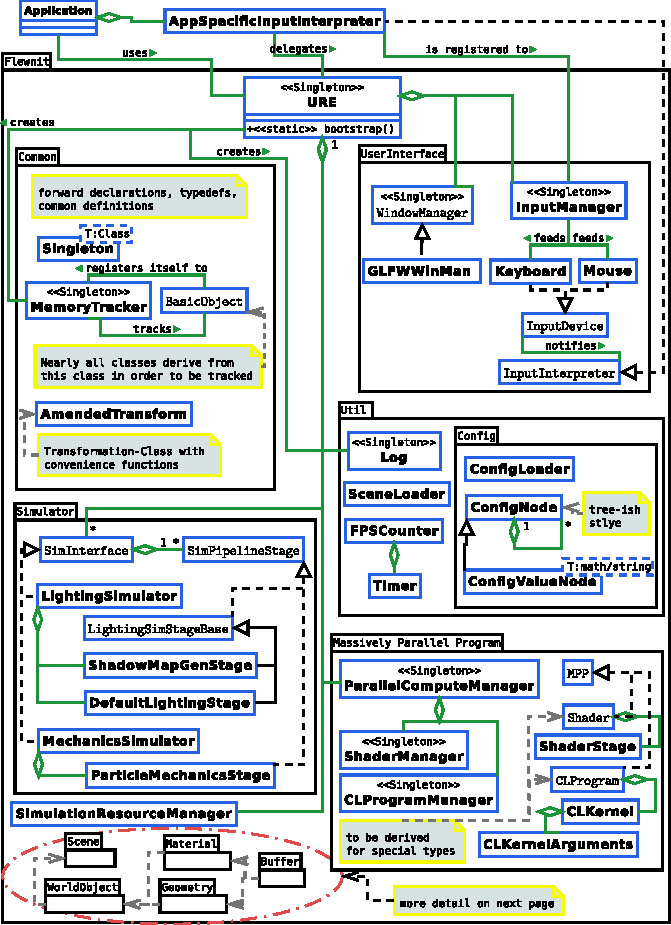
\includegraphics[width=1.09\textwidth]{Overview_Flewnit_Architecture_After_Implementation1.pdf}
	%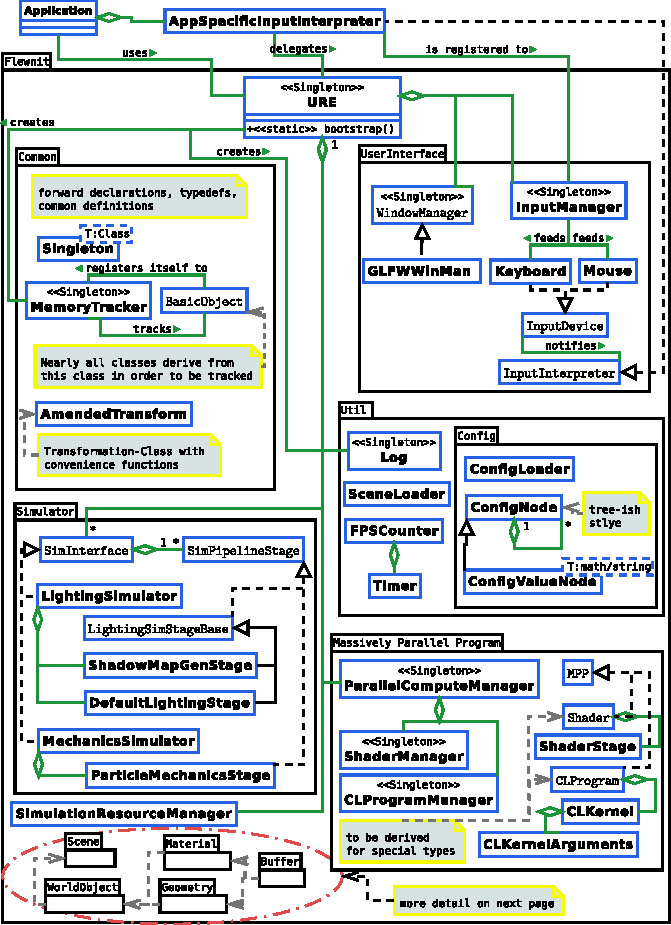
\includegraphics[width=\textwidth]{Overview_Flewnit_Architecture_After_Implementation1.pdf}
	\caption{Klassendiagramm des Gesamtsystems, Teil 1}
	\label{fig:ClassDiagOverview1}
\end{figure}


\begin{figure}[!h]
	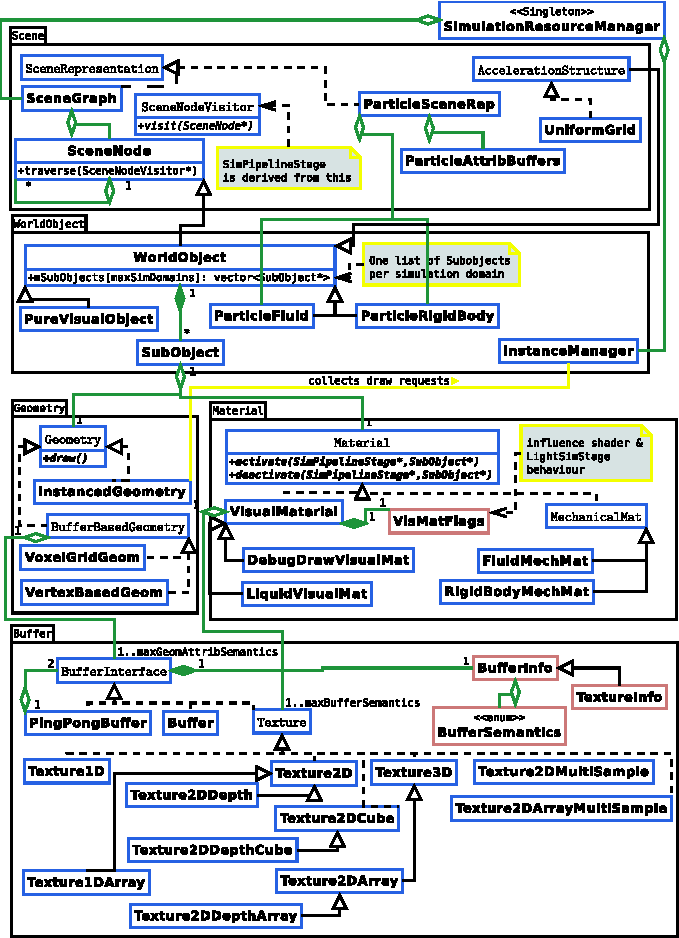
\includegraphics[width=1.09\textwidth]{Overview_Flewnit_Architecture_After_Implementation2.pdf}
	%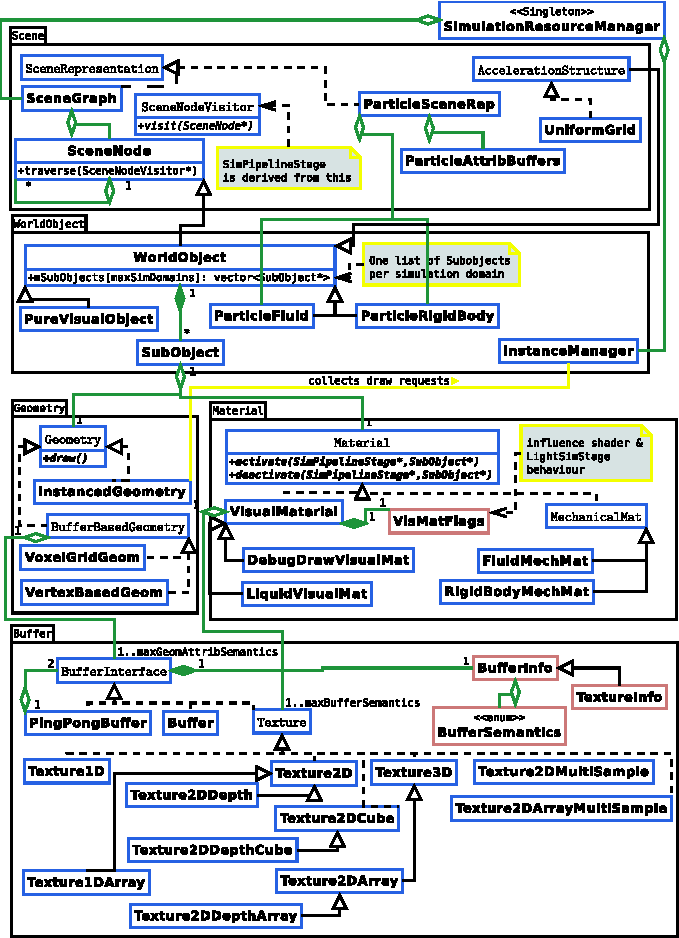
\includegraphics[width=\textwidth]{Overview_Flewnit_Architecture_After_Implementation2.pdf}	
	\caption{Klassendiagramm des Gesamtsystems, Teil 2}
	\label{fig:ClassDiagOverview2}
\end{figure}



Abbildung \ref{fig:ClassDiagOverview1} und \ref{fig:ClassDiagOverview2} zeigen ein vereinfachtes Klassendiagramm
von \emph{Flewnit}. Die roten Klassen stellen wichtige Meta-Informationen dar, um Kontrollfluss und Objekt-Erstellung
zu delegieren. In den folgenden Unterabschnitten werden die einzelnen Komponenten detaillierter vorgestellt.




 
\subsection{BasicObject und Memory Tracking}
	\lstset{language=C++} %we want c++ code listings
	
	Die Bibliothek soll zur Laufzeit kontrolliert herunterfahr- und re-initialisier-bar sein, 
	um eine vielseitige und flexible Anwendung zu gewährleisten. Da bei C++ das Speicher-Management dem
	Programmierer überlassen ist, und man daher vor allem bei massiver Nutzung von Pointern schnell den Überblick
	verliert, 
	\begin{itemize}
		\item welches Objekt welche anderen erschaffen hat
		\item welche Objekte eine Klasse "`besitzt"' und somit für ihre Speicher-Freigabe zuständig ist bzw
		\item auf welche Objekte eine Klasse nur ein Handle für Verwaltung oder	Backtracking hat, ohne für Erschaffung
		 oder Löschung zuständig zu sein
	\end{itemize}
	wurde in Anbetracht der oberen Forderung ein sehr simples Meta-Object-System system realisiert, welches Klassen-Namen
	und Speicherverbrauch eines Objektes feststellt sowie jedem Objekt eine \emph{unique ID} zuweist.
	Zweck dieses Meta Object System-Systems war es, Speicherlecks durch Nicht-Löschen von Objekten während der Entwicklung 
	zu finden;
	
	Dafür erbt beinahe jede Klasse in \emph{Flewnit} von \lstinline|BasicObject|.
	Diese Klasse registriert sich automatisch bei der \lstinline|MemoryTracker|-Singleton-Instanz, bekommt dort eine
	ID zugewiesen. Diese ID hat noch keine Anwendung, könnte sich aber in einem Netzwerk-Kontext als nützlich erweisen.

	Wie bei Qt das \lstinline[language=C++]|Q_OBJECT|-Makro muss in jede von 
	\lstinline[language=C++]|BasicObject| erbende Klasse das Makro 
	\lstinline[language=C++]|FLEWNIT_BASIC_OBJECT_DECLARATIONS| eingetragen werden; Dieses Makro definiert die 
	Implementatoin einer virtuellen Funktion, welche die Meta-Information setzen:
    \begin{lstlisting}
#define FLEWNIT_BASIC_OBJECT_DECLARATIONS \
	public:\
		virtual void initBasicObject() \
		{ \
			mMemoryFootPrint = (int) sizeof(*this); \
			mClassName = String(typeid(*this).name()); \
		} \
	private:	
	\end{lstlisting}
	Diese umständliche Implementierung hat die Urasache, dass Typ-Informationen der Blatt-Klasse einer
	Klassenhierarchie erst dann zur verfügung stehen, wenn alle Konstruktoren der Basis-Klassen zurückgekehrt sind,
	weshalb der obere Code also nicht im Konstruktor der Basisklasse stehen darf, da der \lstinline|this|-Pointer
	noch nicht die Informationen der Blatt-Klasse enthält.
	Ferner, um dem Programmierer nicht zuzumuten, \lstinline|initBasicObject()| in jedem Konstruktor aufzurufen
	(das führt bei tiefen Klassenhierarchien zu unnötigen ausführungen dieser Funktion, da nur die Info der Blatt-Klasse
	benötigt wird, außerdem entstünde so eine weitere Vergesslichkeits-Fehlerquelle, die durch das Meta Object System ja 
	gerade \emph{vermieden} werden soll), stellt der Memory Tracker eine Routine \lstinline|updateMemoryTrackingInfo()|
	bereit, die aufgerufen werden sollte, wenn man auf valide Meta-Information zugreifen will.
	Aufpassen muss man bei tiefen Klassenhierarchien, da hier der Compiler keinen Fehler erzeugt, wenn eine Blatt-Klasse
	das Makro nicht eingetragen hat, da eine Implementierung der Funktion ja bereits durch eine Oberklasse existiert.
	
	Über bedingte Kompilierung lässt sich diese Meta-Funktionalität deaktivieren.
	Ein "`richtiges"' Meta Object System wie das von Qt wollte ich nicht verwenden, da es für meine Zwecke zu komplex und
	mächtig ist, und ich nicht mit Kanonen auf Spatzen schießen wollte. Ohnehin gibt es Tools wie Valgrind, mit denen
	man Speicherlecks finden kann. 

	Letztendlich ist meine Lösung nicht wirklich elegant (auch wenn ich ohne Meta-Object-Compiler (MOC) keine bessere 	
	Lösung gefunden habe) und daher eher als eine Spielerei anzusehen
	mit dem Zwecke, die C++-Interna zu verinnerlichen und zu jeder Zeit daran erinnert zu werden, 
	Destruktoren zu implementieren und sich über 
	"`Besitz- und Verwaltungs-Verhältnisse"' der Klassen Gedanken zu machen.
	
	Der \lstinline|MemoryTracker| verfolgt auch sämtliche Allokationen der \lstinline|BufferInterface|-Klasse,
	also der Basisklasse sämtlicher Buffer-Typen;
	
\subsection{AmendedTransform}
	\label{sec:AmendedTransform}
 	Im Zuge der Überlegungen zum Szenegraphen, der Kamera und des visuellen Renderings vieler Objekte per
 	Hardware-Instancing entschied ich mich, die klassische 4x4-Transformationsmatrix zu wrappen und mit
 	convenience functions anzureichern, siehe Listing \ref{listing:AmendedTransformDef}.\\
 	Der Zweck dieser Klasse ist es, Transformationsmatrizen anhand "`anschaulicher"' Parameter 
 	(Position, Richtung, Up-Vektor, Skalierung) zu definieren,
 	und diese Parameter auch nach Akkumulationen, Modifikationen und/oder Animationen zur Verfügung zu haben.\\
 	Der Fokus liegt hier klar auf der Bequemlichkeit für den Entwickler, nicht auf der Performanz.
 	Sobald sehr große, dynamisch animierte und tiefe Scenegraphen zum Einsatz kommen, könnte diese Klasse
 	zum Flaschenhals werden. Dann ist vielleicht ein Refactoring vonnöten; Vorerst scheint mir die Implementation jedoch
 	angemessen.\\
 	
 	So lässt sich z.B. bequem ein \lstinline|Camera|-Objekt, welches selber von \lstinline|WorldObject| erbt,
 	welches wiederum von \lstinline|SceneNode| abgeleitet ist, an eine andere SceneNode anhängen, und aus der automatisch
 	berechneten globalen Transformation erhält man durch \lstinline|AmendedTransform::getLookAtMatrix()|
 	direkt die lookAt-Matrix, so  dass die Camera-Klasse selber sich nur noch um seine Projektionsmatrix kümmern muss.
 	Auch typische Animationen werden von der Klasse übernommen. Ob dies guter Stil ist, oder doch lieber in die
 	SceneNode-Klasse ausgelagert werden sollte, ist eine Frage, die ich noch nicht abschließend beantworten kann.
 	Es wurde hier dem Paradigma der Datenlokalität gefolgt, evtl. auf Kosten der Separation of Concerns.
 	Eine weitere Erörtertung lasse ich aus, da das Refactoring in diesem Falle nicht zu aufwändig wäre;

	Es sei bemerkt, dass durch die Menge an Matrizen, die an den Vertex Shader beim Instanced Rendering übergeben
	werden müssen, wenn man für alle Fälle gewappnet sein will
	\footnote{z.B. für Layered Rendering in verschiedene Texturen, z.B in ein Textur-Array zur Generierung mehrerer 
	Spotlight-Shadowmaps mit einem Draw-Call; Hierbei braucht es explizit nur die Model-Matrix, da es pro Layer 
	verschiedene View-Matrices (pro Spotlight eine) gibt, von daher nicht im Vorfeld eine ModelView Matrix akkumuliert 
	werden kann}, nicht unerheblich ist, da für jede Instanz ein anderes Matrix-Set übergeben werden muss;
	Die Menge an Daten, die per Uniform-Variable übergeben werden kann, ist begrenzt, daher hängt die maximale Anzahl
	an Instanzen, die pro Draw-Call gezeichnet werdne können, direkt davon ab, wie viele Daten pro Instanz übergeben 
	werden müssen;\\
	Dieser Umstand hat mich dazu verleitet, die Normal Matrix, die transponierte Inverse der ModelView-Matrix,
	"`einzusparen"': da Normalen und Tangenten durch Interpolation für den Fragment Shader ohnehin normalisiert werden 
	müssen, spielt beim Ergebnis  der Transformation eines Vektors 
	\footnote{mit homogener Koordinate 0,im Gegensatz zu Punkten, homog. Koord. 1} 
	nur die Richtung eine Rolle, nicht der Betrag. Die Richtung ändert sich nicht,
	wenn eine uniforme Skalierung in der Matrix steckt, wenn also der Skalierungsfaktor pro Raumdimension überall gleich 
	ist. Der Translations-Anteil einer Matrix spielt bei Vektoren keine Rolle. Aus diesen Umständen lässt sich folgern, 
	dass man zur Transformation von Vektoren ebenfalls die Model- bzw ModelView- Matrix verwenden kann, 
	und \emph{keine} dedizierte Normal Matrix braucht,
	solange nur Translation, Rotation und uniforme Skalierung in der Matrix akkumuliert sind.\\
	Eben dies versuche ich, durch die \lstinline|AmendedTransform|-Klasse zu forcieren, indem nur ein eingeschränkter
	\lstinline|public|-Konstruktor existiert, direkte Initialisierung per Matrix-Konstruktor nur für bestimmte
	\lstinline|friend|-Klassen erlaubt sind, und auch dann diese Matrix validiert wird.
	Die Einschränkung erscheint mir legitim, da eine Uniform Rendering Engine den Anspruch hat, zumindest
	im Ansatz "`physikalisch basiert"' zu sein; Deshalb sollten sich  Skalierungen ohnehin nur selten
	zur Laufzeit ändern, und dann nur einheitlich. So kann man im Vorfeld die Geometrie so anpassen, 
	dass keine nicht-uniforme Skalierung in der Transformationsmatrix auftaucht.
	
	
	Eine \lstinline|AmendedTransform| ist insofern mit der \lstinline|SceneNode|-Klasse verzahnt, dass falls eine
	\lstinline|AmendedTransform|-Instanz als Tranformation einer Scene-Node dient, erstere ein Handle auf die Scene Node 
	bekommt. Auf diese Weise kann die Scene Node immer automatisch informiert werden, wenn sich bei der 
	\lstinline|AmendedTransform| etwas geändert hat (es müssen dann ggfs. die Kinder der Scene-Node aktualisiert werden,
	z.B. für eventuelles Updade von Bounding Boxes). Auf diese Weise muss weder die \lstinline|AmendedTransform|
	nochmal durch die \lstinline|SceneNode| gewrappt werden, noch können Seiteneffekte durch direkte Manipulation der 
	Transformation auftreten, sollte der Programmierer vergessen, anschließend die Scenenode über ihre 
	Transformations-Änderung zu informieren.
	Die Scene-Node-Kopplung ist rein intern, und braucht den Benutzer der Klasse nicht weiter zu interessieren,
	außer in der Hinsicht, dass Scene-Node-Manipulation direkt geschieht und die \lstinline|SceneNode|-Klasse
	kein eigenes Interface zur manipulation von Tranformationen bereit stellt.
	
 	
 	\begin{lstlisting}[caption={AmenededTransform Klassendefinition, gekürzt},label=listing:AmendedTransformDef]
class AmendedTransform
{
public:
	AmendedTransform(
			const Vector3D& position = Vector3D(0.0f,0.0f,0.0f),
			//(0,0,-1) is assumed as initial orientation, extress any deviation in euler angles(radians)
			const Vector3D& direction = Vector3D(0.0f,0.0f,-1.0f),
			const Vector3D& upVector = Vector3D(0.0f,1.0f,0.0f),
			float scale = 1.0f);
	AmendedTransform(const AmendedTransform& rhs);
	virtual ~AmendedTransform();

	AmendedTransform operator*(const AmendedTransform& rhs)const;
	//the assignment operators copy only the transformation values, not the SceneNode-Related info
	const AmendedTransform& operator*=(const AmendedTransform& rhs);
	const AmendedTransform& operator=(const AmendedTransform& rhs);

	//accum: translationMatrix * rotationMatrix * scaleMatrix;
	const Matrix4x4& getTotalTransform()const;
	//convenience functions:
	//unscaled, i.e. orthonormal rotation matrix:
	Matrix3x3 getRotationMatrix()const;
	//inverse of (translationMat*rotationMat);
	Matrix4x4 getLookAtMatrix()const;
	Matrix4x4 getScaleMatrix()const;
	Matrix4x4 getInverseScaleMatrix()const;
	static bool matricesAreEqual(const Matrix4x4& lhs, const Matrix4x4& rhs);
	AmendedTransform getInverse()const;

	/*... getter and setter for pos, dir, up omitted */ 

	//"animation" functions:
	void moveRelativeToDirection(float forwardBackward, float rightLeft, float upDown);
	//change direction by rotating it angleDegrees degrees around cross(direction,upVector)
	void pitchRelativeToDirection(float angleDegrees);
	//change direction by rotating it angleDegrees degrees around the upVector;
	void yawRelativeToUpVector(float angleDegrees);

protected:
	//backtrace pointer to tell the scene node to update itself after its transform has been modified directly;
	//mOwningScenNode->transformChanged(bool global) will be called by any setter function of this class if there is an
	//associated SceneNode;
	SceneNode* mOwningSceneNode;
	//flag needed by Scene node to update itself appropriately
	bool mIsGlobalTransform;
	
	friend class SceneNode;
	void setOwningSceneNode(SceneNode*node, bool isGlobalTransform)
		{mOwningSceneNode = node; mIsGlobalTransform=isGlobalTransform;}


	Vector3D mPosition;
	Vector3D mDirection;
	Vector3D mUpVector;
	float mScale;
	
	Matrix4x4 mAccumTranslationRotationScaleMatrix;

	//construct the transformation matrix from current pos,dir,up,scale; is called by any constructor and related setter;
	//validates members, if possible
	void setup();


	friend class Loader;//the loader may set transformation matrices, as they are read directly from Scene descriptions ;)
	//protected matrix-constructor to omit that the user passes a non-conforming matrix	
	AmendedTransform(const Matrix4x4& transform);
	
};
 	\end{lstlisting}
 	
 	

    	
    	
    	
\subsection{Die \emph{Unified Rendering Engine} (URE)}
	Dies ist die Singleton-Klasse, die sämtliche Komponenten besitzt/verwaltet, und über welche direkt oder indirekt alle 
	Daten beschafft oder Funktionalität aufgerufen werden kann, die nach außen hin verfügbar sein soll.

\subsection{Das UserInterface-Paket}
	Das User Interface hat einen abstraktes Window-Manager-Interface, welches von einer Implementation, die \emph{GLFW} 	
	verwendet, realisiert wird;
	Aus der geparsten Config wird die gewünschte OpenGL-Kontext-Version, Auflösung, Multisamples-Count, Fullscreen-Option
	etc. ausgelesen und ein entsprechendes Fenster mit OpenGL-Kontext erzeugt.\\

	Die Input-Verwaltung ist im Gegensatz zum Fenstermanager nicht vollständig von der verwendeten Input-Bibliothek 	
	(ebenfallse GLFW) abstrahiert, da beim Parsen des Inputs die von GLFW definierten Makros direkt verwendet werden, 
	 wie z.B \lstinline|GLFW_KEY_ENTER|.
	Da die Austauschbarkeit von verwendeten Bibliotheken zwar erwünscht ist, aber ich mich nicht verzetteln wollte,
	bleibt die Abstraktion des Inputs noch ein langfristiges "`TODO"' mit geringerer Priorität.

	Eine GUI wurde leider noch nicht implementiert, vor allem aus dem Grund, dass vorhandene GUI-Toolkits wie z.B.
	\emph{AntTweakBar}\footnote{http://www.antisphere.com/Wiki/tools:anttweakbar} Legacy-OpenGL-Routinen verwenden,
	was die Verwendung eines modernen Core-Profiles ausschließen würde.
	Da langfristig ein konsistentes Erscheinungsblid angestrebt wird, welches seine GUI vollständig in das 
	OpenGL- Rendering-Fenster integriert hat, kam auch die  Verwendung von GUI-Toolkits wie dem von Qt nicht in Frage.\\
	Letztendlich wollte ich schon immer mal eine kleine GUI entwickeln, wozu ich jedoch erwartungsgemäß im Rahmen dieser
	Arbeit keine Zeit hatte. Die GUI verbleibt also als ein "`TODO"' von mittlerer Priorität.




\subsection{Das Simulator-Paket}

	\begin{figure}[!h]
		 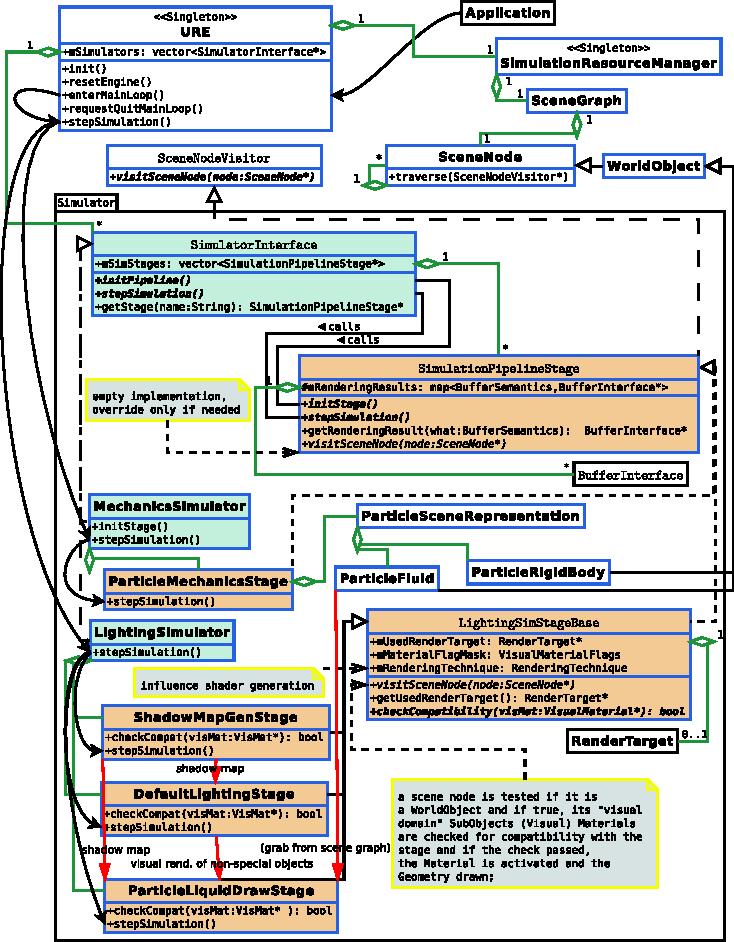
\includegraphics[width=1.15\textwidth]{Detail_Simulator.pdf}
		\caption{Grobes Beispiel von einer Simulation und den zugehörigen Daten-Abhängigkeiten}
		\label{fig:detailSimulator}
	\end{figure}


	Wie bereits erwähnt, soll jede Simulationsdömane einen eigenen Simulator haben, 
	der eine eigene Pipeline an Simulations-Stages verwaltet.
	Es kann theoretisch beliebig viele Simulationsdomänen geben. Momentan sind jedoch nur drei
	über einen \lstinline|enum| definiert: Die visuelle, mechanische und akustische Domäne, wobei
	die akustische Domäne noch nicht in der prototypischen Implementierung vorkommt.
	Abb. \ref{fig:detailSimulator} zeigt grob beispielhaft den Ablauf einer Simulation und die verschiedenen
	Varianten, wie man sich die "`Rendering Results"' anderer Stages beschaffen kann:\\
	Entweder aus der Main Loop der Engine heraus oder von der benutzenden Applikation wird
	\lstinline|URE::stepSimulation()| aufgerufen; Diese Funktion iteriert in fester Reihenfolge über die
	vorhandenen Simulatoren und ruft deren \lstinline|stepSimulation()|-Routine auf; Hierin werden Simulator-
	spezifische Operationen ausgeführt (Framebuffers des Fensters resetten und Haupt-Viewport setzen beim 
	\lstinline|LightingSimulator|, CL/GL-shared Buffers für OpenCL akquirieren beim \lstinline|MechanicsSimulator|...),
	dann über die einzelnen zugehörigen \linebreak
	\lstinline|SimulationPipelineStage|'s iteriert, widerum deren 
	\lstinline|stepSimulation()|-Methode aufgerufen.
	Hier passiert dann das eigentlich \emph{generische Rendering}.
	So verschieden die Algorithmen sind, die in den einzelnen Stages abgearbeitet werden, so verschieden sind auch
	die Möglichkeiten, wie einzelne Stages miteinander Daten austauschen: Der generischste Ansatz ist, sich von einer
	Stage einen Buffer mit einer bestimmten Semantik zu beschaffen, sofern die entsprechende Stage ein solchen
	bereit stellt. Bei Lichtsimulation, die viel mit Texturen und OpenGL-Framebuffer-Objects (FBOs) umgeht,
	bietet sich an, sich das \lstinline|RenderTarget| (die Abtraktion des FBO in \emph{Flewnit}) zu beschaffen,
	um mit dem gesamten RenderTarget weiter zu arbeiten, oder sich einzelne Texturen zu beschaffen.
	Es gibt aber auch die relativ indirekte Methode des Datenaustausches, wie es z.B. zwischen der 
	\lstinline|ParticleMechanicsStage| und der \lstinline|ParticleLiquidDrawStage| der Fall ist: Die Buffer mit dem 		
	physikalischen Attributen sind in der SceneNode-abgeleiteten
	Klasse \lstinline|ParticleFluid| enthalten, so dass die aktualisierten Daten über schlichtes Szenegraphen-Traversieren
	beschafft werden können.\\
	Details zum Ablauf der Simulation(en) werden in Kapitel \ref{sec:simulation} behandelt.




\subsection{Der SimulationResourceManger}
	Diese Singleton-Klasse besitzt und verwaltet die Assets,\linebreak 
	als \lstinline|std::map<String,X*>| für Referenzierung über einen Namen, 
	wobei \lstinline|X| folgende Klassen betrifft: 
	\begin{itemize}
		\item \lstinline|Material|
		\item \lstinline|Geometry|
		\item \lstinline|BufferInterface|
		\item \lstinline|Texture| \footnote{Da \lstinline|Texture| von \lstinline|BufferInterface| erbt, 
		handelt es sich um eine Handle-Sammlung der Untermenge der Texturen aller \lstinline|BufferInterface|s,
		um einen bequemeren Zugriff zu ermöglichen}
		\item \lstinline|InstanceManager|
	\end{itemize}
	Außerdem bestitzt die Klasse den \lstinline|SceneGraph| und stellt einen Handle auf den aktuellen 
	\lstinline|SkyDome| zur Verfügung, so dass alle Objekte ein konsistentes Environment Mapping 
	betreiben können, sofern dies erwünscht ist.

		
\subsection{Das Scene-Paket}		
	Neben dem klassischen Szene-Graphen, der vor allem im Kontext des visuellen Echtzeit-Rendering verwendet wird,
	da er Culling und relative Transformationen ermöglicht, 
	erfordern verschiedene Simulationsdomänen und Repräsentationen der beteiligten Simulations-Objekte
	(z.B. als Dreiecks-Mesh, Komposition von komplexeren Primitiven, Punktwolke oder Voxel-Grid)  ggfs. 
	unterschiedliche Szene-Repräsentationen, damit die spezifischen Anforderungen der Simulation als solchen und der
	Respräsentation der simulierten Objekte optimal erfüllt sind.\\
	Diese Szenen-Repräsentationen unterscheiden sich in der logischen Organisation ihrer Objekte 
	(z.B. Baumstruktur, sortierte oder unsortierte Sammlung, Graph-Struktur, Voxel-Struktur) 
	und in den Meta-Informationen, welche für die einzelnen	Objekte notwendig sind.
	
	Beispielsweise stellt die die effiziente Suche nach räumlich benachbarten Objekten eine wichtige Anforderung
	bei vielen Simulationen (auch bei Lichtsimulation für globale Beleuchtungseffekte) dar.
	Hierfür bieten sich verschiedene Beschleunigungsstrukturen an. Je nach Simulationsdomäne, 
	Objekt-Repräsentation,verwendetem Simulations-Verfahren, verwendeter Hardware und Zielsetzung 
	(Geschwindigkeit, Genauigkeit, Speicherverbrauch...) sind verschiedene Beschleunigungsstrukturen angemessen.
	Somit besteht keine 1:1-Verbindung zwischen Szenen-Repräsentation und Beschleunigungsstruktur.\\
	Beschleunigungsstruktur und Szenen-Repräsentatioen sind somit nur lose gekoppelt.
	Um die verschiedenen Zwecke zu verdeutlichen, stellt Tabelle \ref{tab:sceneRepVsAccStruct} diese gegenüber.


	\begin{table}	 	
	 	\begin{tabular}
  		{ x{0.33\textwidth} | x{0.33\textwidth} | x{0.33\textwidth} | }	
  					\cline{2-3}
  					& Szenen-Repräsentation & Beschleunigungsstruktur
  					\tabularnewline\cline{1-3}
  		\multicolumn{1}{ |c| }{
  			Organisation der Elemente
  		}			&	
  						logisch für Zugriff auf Ebene der Anwendungslogik
  					&  
						räumlich für effizienten Zugriff durch einen Simulations-Algorithmus
  			 		\tabularnewline\cline{1-3}
   		\multicolumn{1}{ |c| }{
  			Zweck von Meta-Informationen
  		}			&
  						verschieden, je nach Repräsentation und Typ der Simulations-Objekte	
  					&	
  						(sofern vorhanden) unterschliedlich für verschiedene Algorithmen, z.b.
 						effiziente Traversierung und/oder Nachbarschaftssuche
  					\tabularnewline\cline{1-3}	  	  	
	  	\end{tabular}	  	
  		\caption{Gegenüberstellung der Zwecke einer generischen Szenen-Repräsentation und einer Beschleunigungsstruktur}
  		\label{tab:sceneRepVsAccStruct}
	\end{table}	
	
	Es gibt also zwei Basis-Klassen, wie in Abb. \ref{fig:ClassDiagOverview2} zu sehen ist:
	\lstinline|SceneRepresentation| und \lstinline|AccelerationStructure|.
	\lstinline|AccelerationStructure| erbt von \lstinline|WorldObject|(siehe Abschnitt \ref{sec:worldObject}),
	um optional Debug-Draw-Funktionalität bereit zu stellen.
	Ansonsten handelt es sich schlicht um abstrakte Basis-Klassen ohne weitere Funktionalität.
	
	Für das gesamte System über den \lstinline|SimulationResourceManger| verfügbar ist der
	\lstinline|SceneGraph|. Dieser enthält die Wurzel-\lstinline|SceneNode|, welche beliebig viele Kinder derselben
	Klasse haben kann. Somit wird eine Baumstruktur gebildet.\\
	Die SceneNode bildet die Basis-Klasse des \lstinline|WorldObject| (siehe Abschnitt \ref{sec:worldObject}).
	
	Es ist ein Mechanismus konzipiert, sowohl Kinder als auch Vorfahr über Änderungen der eigenen Transformation
	und/oder Bounding Box zu informieren, so dass ggfs. globale Transformationen akkumuliert werden können und/oder
	die Bounding Box für den eigenen Unterbaum ermittelt, die für Culling-Berechnungen verwendet werden kann.
	Noch ist dieses Feature nicht in Nutzung und seine Implementation unvollständig und ungetestet,
	daher wird auf weitere Details	verzichtet.
	
	Die klassischen Operationen (Einfügen, Aushängen, rekursives Suchen im Unterbaum nach Namen, Node bewegen,
	Transformationen akkumulieren) sind jedoch implementiert. Es sei an die enge Kopplung dieser Klasse an
	\lstinline|AmendedTransform| (s. Abschnitt \ref{{sec:AmendedTransform}}) erinnert.
	
	Der Scenegraph kann nach dem Visitor- Design Pattern traversiert werden. Z.B. erbt 
	\lstinline|SimulationPipelineStage| von \lstinline|SceneNodeVisitor|, so dass bei Bedarf eine Pipeline-Stage
	nur \lstinline|virtual void visitSceneNode(SceneNode* node)| implementieren muss, um Operationen auf oder mit
	den Objekten des Szenegraphen auszuführen.
	Momentan "`besitzt"' die \lstinline|SceneNode|-Klasse seine Kinder, was den Vorteil hat, dass die Nodes nicht woanders
	verwaltet werden müssen, aber den Nachteil, dass ausgehängte Scene Nodes nicht automatisch beim Reset der Engine
	gelöscht werden. Sollte sich dies später als Problem herausstellen, könnte man die Scene Nodes auch vom
	\lstinline|SimulationResourceManger| verwalten lassen.
	Auch empfiehlt sich langfristig die Möglichkeit zur Erschaffung und Verwaltung mehrerer Szenegraphen.
	Aus Zeitgründen habe ich es jedoch erstmal bei dieser rudimentären Implementation belassen.
	
	Intern verwaltet die \lstinline|ParticleMechanicsStage|, die \lstinline|SimulationPipelineStage|,
	die im \lstinline|MechanicsSimulator| für die partikelbasierte Simulation zuständig ist, 
	eine \lstinline|ParticleSceneRepresentation|. Diese verwaltet 
	\begin{itemize}
		\item die "`makroskopischen Objekte"', die an dieser Simulation teilnehmen,
		namentlich (allesamt von \lstinline|WorldObject| abgeleitete) 
		partikelbasierte Fluide, partikel-repräsentierte Rigid Bodies und statische Kollisions-Meshes
		\footnote{diese müssen in einem bestimmten Format vorliegen}
		\item die einzelnen Attribute-Buffers der Partikel
			(Position, Dichte, Geschwindigkeit, Beschleunigung usw.)
		\item Buffers mit Meta-Informationen der "`makroskopischen Objekte"', die an OpenCL-Kernels übergeben werden
	\end{itemize}
	Ferner stellt die Klasse Factory-Methoden für die makroskopischen Objekte bereit, da diese direkt mit den
	Partikel-Buffern assoziiert sind, sich also alle beteiligten Objekte die Buffers teilen müssen. Die korrekte
	Delegierung der Offsets und Sicherstellung der richtigen Größen wird so übernommen.\\
	Die \lstinline|ParticleMechanicsStage| nutzt außerdem ein \lstinline|UniformGrid| für die Simulation.
	Details hierzu werden im Verlauf des Kapitels \ref{sec:mechanicalDomain} beschreiben.
	
	


\subsection{Das WorldObject}
	\label{sec:worldObject}
	Das \lstinline|WorldObject| stellt die abstrakte Basisklasse für sämtliche Objekte dar, mit denen eine oder mehrere 
	Simulationen durchgeführt werden sollen\footnote{Und sei es nur Debug Drawing; Selbst dies kann als eine 
	rudimentäre Form von Lichtsimulation aufgefasst werden.}. Sie erbt von \lstinline|SceneNode|. Damit ist sie bequem 
	in den Szenegraphen integrierbar und hat außerdem schon seinen Transformations-Membervariable.
	
	Bei dieser Klasse zeigt sich erstmals die angestrebte Symmetrie zwischen sen Simulationsdömanen: 
	Für jede Simulationsdomäne
	gibt es eine (möglicherweise leere) Liste an \lstinline|SubObject|'s. Das \lstinline|SubObject| 
	stellt eine Abstraktion dessen dar, was in einer klassischen Graphik-Engine ein "`SubMesh"' oder
	in einer klassischen Physik-Engine eine Komponente einer "`(Compound) Collision Shape"' sein könnte.\\
	Ein \lstinline|SubObject| hat immer einen Pointer auf genau ein \lstinline|Material|, 
	eine \lstinline|Geometry|  und für Backtracking-Zwecke auf sein besitzendes	\lstinline|WorldObject|.
	Wie der Backtracking-Pointer andeutet, besitzt das ein \lstinline|WorldObject| jedes seiner \lstinline|SubObject|s.
	Die vom \lstinline|SubObject| genutzte Geometrie und Materialien können jedoch --sofern sinnvoll -- von beliebig
	vielen \lstinline|SubObject|s gemeinsam genutzt werden.
	
	Es sind verschiedenste Ableitungen von \lstinline|WorldObject| denkbar, z.B. 
	(standard/particle based/voxel based) Rigid Body, Soft Body, rein visuelles Objekt,  
	Kamera,Lichtquelle, Debug-Draw-Objekte, Cloth, Hair, oder (particle based/voxel based) Fluid.
	
	Welche Objekte im Szenegraph für die Nutzung in einer Simulations-Stage in Frage kommen, lässt sich entweder
	über eine Vorfilterung bei Objekt-Erstellung (Factory-Pattern oder automatische Registierung bei einer 
	Manager-Klasse im Konstruktor), oder über \lstinline|dynamic_cast<>()|'s und anschließendes Auslesen von spezifischer
	Meta-Information ermitteln, oder aber durch "`property flags"', also Bit-Flags, die Features einer Scene Node andeuten.
	Welche dieser Methoden langfristig die robusteste, flexibelste und eleganteste ist,
	vermag ich noch nicht zu sagen. Da Typ-Informationen über \lstinline|enum|s 
	(als Bitflags oder "`normale"' Aufzählungstypen)
	eine gewisse Redundanz hat ggü. der dynamischen Typ-Information, die C++ bereit stellt, und außerdem eine weitere
	Fehlerquelle für den Programmierer darstellt, sind die Bitflags nicht erste Wahl. Außerdem schränkt die explizite 
	Auflistung von Features womöglich die Erweiterbarkeit des Systems ohne komplette Neu-Kompilierung ein.
	Andererseits machen sie Programme vielleicht lesbarer, indem bestimmte Kategorien/Features explizit aufgelistet 
	(und im Falle von Bitflags beliebig kombinierbar) sind, 
	und nicht implizit in C++-Typinformationen codiert sind.
	Ich verwende Aufzählungstypen intensiv in \emph{Flewnit}. Nicht immer sind diese für die Programmlogik nötig.
	Sie halfen mir jedoch zur Strukturierung und Ideen-Sammlung. Letztere ist wichtig, da bei einem Softwaresystem,
	welches generische Verwendbarkeit anstrebt, schon weit vor Implementierung konkreter Klassen die Struktur der
	Basisklassen anhand von abstrahierten (erwarteten) gemeinsamen Features der möglichen abgeleiteten Klassen
	möglichst exakt bestimmt werden sollte. Je weiter oben in der Klassenhierarchie Design-Fehler auftauchen, desto
	aufwändiger droht das spätere Refactoring zu werden.

%	Die Entscheidung, dass \lstinline|WorldObject| abstrakt sein soll, wurde getroffen, damit keine Funktionalität,
%	die zunächst generisch erscheint, sich aber später als doch nicht allgemein auf alle konkreten 
%	\lstinline|WorldObjects| anwendbar herausstellt, diese Basisklasse verunreinigt. 
%	Es sind so viele verschiedenste Ableitungen denkbar (Rigid Body, Soft Body, rein visuelles Objekt, Kamera,
%	Lichtquelle, Debug-Draw-Objekte, Cloth, Hair, Fluid...)	
  
 
\subsection{Material}  

	Der Begriff "`Material'", der sich in der Computergraphik eingebürgert hat als Beschreibung von visuellen Eigenschaften
	einer Oberfläche, erscheint mir prädestiniert, sich in seiner Bedeutung in einem alltäglichen,
	nicht computergraphischen Kontext wieder anzunähern:
	das \emph{Material} in \emph{Flewnit} steht für "`sämtliche Eigenschaften von Materie 
	außer ihrer geometrischen Form und internen Repräsentation dieser"'.

	\begin{figure}[!h]
		\centering
	   	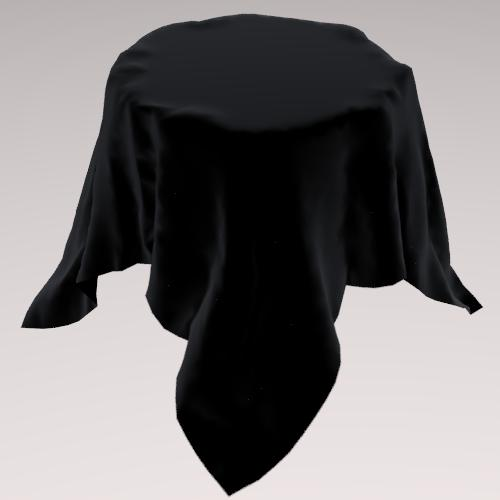
\includegraphics[width=0.3\textwidth]{velvetBlack1.jpg}
		\caption{ Der Begriff \emph{Material} mit einer physikalisch orientierten Bedeutung:
			sämtliche Eigenschaften von Materie	außer ihrer geometrischen Form.
			(Bild entnommen aus \cite{microfacet})
		}
		\label{fig:material}
	\end{figure}
	
	Würden wir über die entsprechende Rechenleistung verfügen und als Programmierer das physikalische Know-How
	besitzen (z.b. über Maxwell'sche Gleichungen), bräuchte man dieses Konzept gar nicht weiter zu konkretisieren,
	und könnte sämtliches Verhalten von Simulations-Objekten durch subatomare Material-Eigenschaften modellieren.
	Dies wäre eine "wirkliche" Vereinheitlichung der bestehenden Engine-Konzepte, die unserer Realität Rechnung trüge.
	Da wir jedoch realistisch (im Sinne der Machbarkeit) bleiben wollen jetzt und heute Echtzeit-Fähigkeit,
	auch auf Kosten von physikalischer Korrektheit/Genauigkeit anstreben, sind Domänen-spezifische Konkretisierungen des
	Material-Konzeptes notwendig, und wie so viele andere Klassen in diesem System wird die 
	\lstinline|Material|-Klasse zur abstrakten Oberklasse.
	Bei einem \lstinline|SubObject|, welches der visuellen Simulationsdömane angehört, wird implizit erwartet,
	dass das genutzte \lstinline|Material| ein \lstinline|VisualMaterial| ist 
	(mit Texturen, Shader, und verscheiedenen Meta-Informationen, um das visuelle Rendering zu delegieren,
	siehe Abschnitt \ref{sec:visualMaterial}), 
	und in der mechanischen Domäne muss es ein \lstinline|MechanicalMaterial|(mit Eigenschaften wie Masse, Reibung, 	
	Elastizität etc.) sein. Diese domänenspezifischen Material-Typen können oder müssen (je nach Typ des nutzenden
	\lstinline|WorldObject|s) noch weiter abgeleitet sein.
	
	Einen etwas schalen Beigeschmack haben die Routinen:
	\begin{lstlisting}
virtual void activate(
		SimulationPipelineStage* currentStage,
		SubObject* currentUsingSuboject) throw(SimulatorException){}
//undoing stuff, like re-enable depth test etc.
virtual void deactivate(SimulationPipelineStage* currentStage,
		SubObject* currentUsingSuboject) throw(SimulatorException){}
	\end{lstlisting}
	Sie sind dem Statemachine-basierten visuellen Rendering mit OpenGL zu verdanken und müssen daher von den
	\lstinline|VisualMaterial|-Klassen implementiert werden. Um der Möglichkeit Rechnung zu tragen, dass
	ähnlich State-basierte Mechanismen an anderer Stelle als beim OpenGL-Rendering vorkommen sollten, sind diese
	Routinen in die Oberklasse gelangt.

	

    	
\subsection{Die Buffer-Abstraktion}  
	%Abschnitt ausgelagert weil er zu groß wurde!
	\label{sec:architecture:BufferAbstraction} 	

	Logischerweise müsste nun eigentlich 
	-- der Top-Down-Präsentation der einzelnen Pakete und Klassen entsprechend --
	die \lstinline|Geometry|-Klasse vorgestellt werden. Um letztere Klasse jedoch besser zu verstehen,
	ist die Kenntnis der Buffer-Abstraktion vorteilhaft. Die \lstinline|Geometry| wird in \ref{sec:geometry} beschrieben.
	
	Wie auf Seite \pageref{overview:bufferAbstraction} erwähnt, abstrahiert die \lstinline|BufferInterface|-Klasse
	sämtliche Buffer-bezogene Funktionalität, namentlich für Host-Buffer, OpenCL-Buffer, 
	verschiedene OpenGL-Buffertypen und letztendlich verschiedene Texturtypen (eine Teilmenge davon ist OpenCL-interop-
	kompatibel bzw als reine OpenCL-Textur erschaffbar).
	Es ergibt sich ein wahrer Moloch, der für eine relativ einheitliche Handhabung zu abstrahieren ist: 
	
	\begin{itemize}
		\item verschiedene APIs (OpenGL C-Api "`vs."' OpenCL C++-API)
		\item verschiedene Verwendungen und Verfügbarkeiten schon allein von non-Textur-Buffern 
			(generisch, Vertex Index/Vertex Attribute Buffer, Uniform Buffer, Render Buffer),
			siehe Tabelle \ref{tab:bufferSupportInContexts}
		\item verschiedene OpenGL-Texturtypen mit nur bedingt kombinierbaren und nur teilweise zu OpenCL kompatiblen 
			erweiterten  Features, siehe Tabelle \ref{tab:textureTypes} 
			%(Tiefentextur ja/nein, MipMapping ja/nein, Textur-Array ja/nein, Multisample-Texture ja/nein, 
			%Rectangle Texture ja/nein, Cube Map ja/nein)
		\item verschiedene Datenformat/Channel-Layout-Deskriptoren, siehe Listing \ref{listing:BufferElementInfo}
	\end{itemize}	
	
	Es hat schon sehr viel Zeit gekostet, sich aus den Spezifikations-Dokumenten 
	(\cite{openGL_4_1_Spec}, \cite{openCL_1_0_Spec}) die möglichen Permutationen, Zusammenhänge, Entsprechungen
	und unterstützten Operationen zu erarbeiten 
	(siehe Tabellen \ref{tab:channelLayoutAndTypes} und \ref{tab:textureTypes}).
	
	Die Ergebnisse dieser Tabellen flossen in die Entscheidung ein, welche konkreten Buffer-
	und Textur-Klassen mit welchen  verfügbaren Features durch Ableitung vom
	\lstinline|BufferInterface| implementiert wurden. Die Konstruktor-Parameter sollten
	so spezifisch zugeschnitten sein, dass der Benutzer der Klassen möglichst wenig invalide
	Kombinationen angeben kann. Außerdem sollte er sich nicht um all die Makros
	wie \lstinline|GL_RGBA32UI| bzw \lstinline|CL_RGBA| und \lstinline|CL_UNSIGNED_INT32|
	kümmern müssen 
	\footnote{Was in OpenCL getrennt ist und somit "`nur"' 
		4 Channeltypen \emph{+} 3 Bitgrößen * (3 non-normalized + 2 normalized)= theoretisch 19 makros ergibt,
		braucht bei OpenGL
			4 Channeltypen \emph{*} 3 Bitgrößen * (3 non-normalized + 2 normalized)= theoretisch 60 makros;
			Erstens stört die Asymmetrie, zweitens das "`Zusammenklatschen"' eigentlich unabhängiger Parameter in ein 
			Makro}. 
	Es soll ein Buffer mit einem einzigen Konstruktor-Call völlständig definiert,
	falls erwünscht auf dem Host-Memory und -- sofern unterstützt --
	in den gewünschten API-Contexten allokiert bzw registiert werden.
	
	Hierfür mussten einige \lstinline|enum|s und Meta-Info-Klassen/Structures definiert werden:
	\begin{description}
		
		\item[enum Type] 
		Beschreibt String-, boolsche, Skalar-, Vektor- und Matrix-Datentypen mit verschiedener 
		Genauigkeit. Findet in \emph{Flewnit} u.a. auch beim Config-Parsen Verwendung.
		
		%--------------------------------------------------------------------------------------------
		\item[enum ContextType und ContextTypeFlags] 
		Mithilfe dieser Datentypen lässt sich spezifizieren, in welchem 
		Kontexten (Host, OpenGL, OpenCL) man einen Buffer erstellt/allokiert/registriert haben will.
		
		%--------------------------------------------------------------------------------------------
		\item[enum BufferSemantics] 
		Eine sehr wichtige Auflistung konkreter Verwendungszwecke des Buffers,
		siehe Listing \ref{listing:BufferSemantics} im Anhang \ref{append:bufferListings}.
		Dieser Aufzählungstyp ist eine große Erleichterung beim Hantieren mit OpenGL Vertex Buffer Objects (VBO's) 
		\footnote{abstrahiert von \lstinline|Flewnit::VertexBasedGeometry|, s. \ref{sec:geometry} }
		und Frame Buffer Objects (FBO's) 
		\footnote{abstrahiert von \lstinline|Flewnit::RenderTarget|}, 
		da hier zur Assoziation von VBO-Vertex Attribute Buffern mit Input-Variablen im Vertex Shader
		bzw and FBO gehängte Texturen mit Output-Variablen im Fragment Shader
		ein Index angegeben werden muss. 
		Wenn wir als Index die numerische Entsprechung der Buffer-Semantik verwenden, 
		ist nicht nur die Lesbarkeit des Codes erhöht, es ist auch automatisch sichergestellt, 
		dass Indizes keine Konflikte versursachen!
		
		%--------------------------------------------------------------------------------------------
		\item[enum GPU\_DataType] Listet nur die von der GPU / OpenGL nativ unterstützten Datentypen auf, ohne
		Präzisions- und Normalisierungs-Information:
		\begin{lstlisting}		
enum GPU_DataType
{
	GPU_DATA_TYPE_FLOAT,
	GPU_DATA_TYPE_INT,
	GPU_DATA_TYPE_UINT
};
		\end{lstlisting}
		
		%--------------------------------------------------------------------------------------------
		\item[enum GLBufferType]
		Listet die vom Buffer-Interface abstrahierten OpenGL-non-Textur-Buffertypen auf. 
		Aus Zeitgründen und Erwartung, dass sie außerhalb der \lstinline|RenderTarget|-Klasse nicht benötigt werden,
		werden z.B. Render Buffers nicht abstrahiert.
		\begin{lstlisting}		
enum GLBufferType
{
	NO_GL_BUFFER_TYPE,
	VERTEX_ATTRIBUTE_BUFFER_TYPE,
	VERTEX_INDEX_BUFFER_TYPE,
	UNIFORM_BUFFER_TYPE 
};
		\end{lstlisting}	
	
		%--------------------------------------------------------------------------------------------
		\item[struct BufferElementInfo] 
		Beschreibt -- sofern erwünscht bzw nötig -- das Channel-Layout,die Datentypen, die Bit-Genauigkeit
		und die etwaige Normalisierung eines Buffers mit Channels, 
		z.B. einer Textur oder einem Vertex Attribute Buffer,
		siehe Listing \ref{listing:BufferElementInfo} im Anhang \ref{append:bufferListings}.
		Auf diese Weise spart man sich die verschiedenen "zusammengesklatschten", asymmetrischen GL/CL-Makros;
		Die Structure validiert ihre Daten. Diese werden später für die internen CL/GL-API-Aufrufe in die
		entsprechenden CL/GL-Makros transformiert,
		siehe Listing \ref{listing:BufferElementInfoToCLGL} im Anhang \ref{append:bufferListings}.
		
		%--------------------------------------------------------------------------------------------
		\item[struct GLImageFormat]
		OpenCL definiert folgende Structure:
		
		\begin{lstlisting}		
typedef struct _cl_image_format {
    cl_channel_order        image_channel_order;
    cl_channel_type         image_channel_data_type;
} cl_image_format;	
		\end{lstlisting}
		
		Um das interne Handling der CL/GL-Makros etwas symmetrischer zu machen (man verliert leicht den Überblick),
		habe ich ein ähnliches Makro definiert, welches aufgrund der Kommentare im Anhang  \ref{append:bufferListings},
		Listing \ref{listing:GLImageFormat} zu finden ist.\footnote{Die Kommentare geben weiteren Aufschluss über 
		die Asymmetrie der einzelnen APIs: obwohl sie beide von der Khronos Group spezifiziert wurden und explizit 	
		Interoperabilität ermöglichen, stiften viele mehr oder minder kleine Asymmetrien Verwirrung (zumindest bei mir);
		Diese Umstände trugen zu der Entscheidung bei, das \lstinline|BufferInterface| zu entwickeln, trotz des
		erheblichen Zeitaufwands.}
		
		
		\item[class BufferInfo]
		Dies ist die Klasse, die sowohl als "`Construction Info"' den Konstruktor-Code delegiert, als auch für 
		den benutzer später Meta-Information bereitstellt.
		Es sei hier nur der Standard-Konstruktor angegeben:
		
		\begin{lstlisting}	
explicit BufferInfo(String name,
	ContextTypeFlags usageContexts,
	BufferSemantics bufferSemantics,
	Type elementType,
	cl_GLuint numElements,
	const BufferElementInfo& elementInfo,
	GLBufferType glBufferType = NO_GL_BUFFER_TYPE,
	ContextType mappedToCPUContext = NO_CONTEXT_TYPE);
		\end{lstlisting}
		
		Ich muss zugeben, dass \lstinline|elementType| und \lstinline|elementInfo| redundant sind, außerdem diese 
		beiden Parameter eigentlich bei generischen Buffern, wo die Typ-Information zumindest für die GPU Computing APIs
		keine Rolle spielt, fehl am Platze sind. Mangelndem Überblick in der Anfangsphase der Implementierung
		über die Verschiedenen Arten, Buffers in CL und GL zu nutzen, sind diese Design Flaws zuzuschreiben.
		Ein Refactoring mit besser speziell zugeschnittenen Konstruktoren ist geplant.
		zu nutzen
	
	\item[class TextureInfo]
		So wie \lstinline|Texture| von \lstinline|BufferInterface| erbt, erbt auch 
		\lstinline|TextureInfo| von \lstinline|BufferInfo|. Sie stellt die gleiche Funktionalität für
		die (abstrakte) \lstinline|Texture|-Klasse dar wie \lstinline|BufferInfo| für \lstinline|BufferInterface|.
		Ein Unterschied besthet jedoch darin, dass \lstinline|TextureInfo| eigentlich nur dazu dient, 
		die kombinierte Information aus den Parametern der "`eingeschränkten"' Konstruktoren 
		der konkreten Textur-Klassen (\lstinline|Texture2D| etc.) und der inhärent klassenspezifischen
		Eigenschaften an die \lstinline|Texture|-Oberklasse zu übergeben. Damit hat \lstinline|TextureInfo|
		eher eine Textur-interne Funktion bei der Konstruktion. Das tut jedoch seiner Funktion als späterer
		Meta-Daten-Lieferant keinen Abbruch.
		Auch hier reicht der Standard-Konstruktor für eine Idee dieser Klasse:
		 
		\begin{lstlisting}	
explicit TextureInfo(
	const BufferInfo& buffi,
	cl_GLuint dimensionality,
	Vector3Dui dimensionExtends,
	GLenum textureTarget,
	bool isDepthTexture = false,
	bool isMipMapped = false,
	bool isRectangleTex = false,
	bool isCubeTex = false,
	GLint numMultiSamples = 1,
	GLint numArrayLayers = 1
	);
		\end{lstlisting}			
			
	\end{description}	

 	
 	\begin{table}[!h]
  		\begin{tabular}
  		{
  		 l  l | c | c | c |
  		}
																	\cline{3-5}
  									&								&	\multicolumn{3}{ c | }{Context} \\ 
  																	\cline{3-5}
									&								& 	Host 	& 	OpenGL 	& 	OpenCL	\\
    	\noalign{\hrule}								
    	\multicolumn{1}{|c|}{
    		generic Buffer
    	}							& 								
    		&	{\color{green}\checkmark} 	&	{\color{red}x}		& 	{\color{green}\checkmark}	\\ 
    	
    	\noalign{\hrule}								
    	\multicolumn{1}{|c|}{
    		\multirow{4}{*}{OpenGL Buffers}
    	}							& Vertex Attribute Buffer		
    		&	{\color{orange}o} 	&	{\color{green}\checkmark}		& 	{\color{orange}o}	\\  
    								\cline{3-5}
    	\multicolumn{1}{|c|}{}		& Vertex Index Buffer			
    		&	{\color{orange}o} 	&	{\color{green}\checkmark}		& 	{\color{orange}o}	\\  
    								\cline{3-5}
    	\multicolumn{1}{|c|}{}		& Uniform Buffer
    		&	{\color{orange}o} 	&	{\color{green}\checkmark}		& 	{\color{orange}o}	\\ 
    								\cline{3-5} 
    	\multicolumn{1}{|c|}{}		& Render Buffer					
    		&	{\color{red}x} 	&	{\color{green}\checkmark}		& 	{\color{green}\checkmark}	\\ 
    
   		\noalign{\hrule}								
   		\multicolumn{1}{|c|}{
    		\multirow{4}{*}{Textures} 
   		}							& 1D Texture					
   			&	{\color{orange}o} 	&	{\color{green}\checkmark}		& 	{\color{red}x}	\\ 
    								\cline{3-5}
		\multicolumn{1}{|c|}{}		& 2D Texture				
			&	{\color{orange}o} 	&	{\color{green}\checkmark}		& 	{\color{green}\checkmark}	\\ 
									\cline{3-5}
		\multicolumn{1}{|c|}{}		& 3D Texture		
			&	{\color{orange}o} 	&	{\color{green}\checkmark}		& 	{\color{green}\checkmark}	\\ 
									\cline{3-5}
		\multicolumn{1}{|c|}{}		& Special Texture				
			&	{\color{orange}?} 	&	{\color{green}\checkmark}		& 	{\color{orange}?}	\\ 


    	\noalign{\hrule}
     
     	
  		\end{tabular}	
  	
  		\caption{		
  			Verschiedene Buffertypen und ihre Verfügbarkeit in verschiedenen Kontexten \\	
  			Legende: \\
			{\color{green}\checkmark}	$\rightarrow$ nativ unterstützt;
			{\color{orange}o}	$\rightarrow$ kompatibel;
			{\color{red}x}	$\rightarrow$ nicht unterstützt;	\\
			{\color{orange}?}	$\rightarrow$ Unterstützung abhängig von weiteren Parametern, 
								s. Tabelle \ref{tab:textureTypes};	
		}
		\label{tab:bufferSupportInContexts}
  	\end{table}
  	
  	
  	\begin{table}[!h]
  		\begin{tabular}
  		{
  			|l|c|c|c|c|c|
  		}
		\noalign{\hrule}						
  						&	CL interop	&	MipMap	& Depth	&	Array	&	Rectangle	\\
  		\noalign{\hrule}						
  		Texture1D		& {\color{red}x} & {\color{green}\checkmark} & {\color{red}x}
  						& {\color{green}\checkmark} & {\color{red}x} \\
		\noalign{\hrule}						
  		Texture2D		& {\color{green}\checkmark} & {\color{green}\checkmark} & {\color{green}\checkmark}  
  						& {\color{green}\checkmark} & {\color{green}\checkmark} \\
  		\noalign{\hrule}						
  		Texture2DCube 	& {\color{yellow}o} & {\color{green}\checkmark}  & {\color{green}\checkmark}
  						& {\color{orange}o} & {\color{red}x} \\
  		\noalign{\hrule}						
  		Texture2DMultiSample& {\color{red}x} & {\color{red}x}  & {\color{red}x} 
  						& {\color{green}\checkmark} & {\color{red}x} \\	
  		\noalign{\hrule}						
  		Texture3D		& {\color{green}\checkmark} & {\color{green}\checkmark}  & {\color{red}x} 
  						& {\color{red}x} & {\color{red}x} \\
  		\noalign{\hrule}						
  		\end{tabular}
  		
  		\caption{Verschiedene Texturtypen und ihre Kompatibiltät zu bestimmten Features \\	
  			Legende: \\
			{\color{green}\checkmark}	$\rightarrow$ unterstützt;
			{\color{yellow}o}	$\rightarrow$ In OpenCL unterstützt, aber nicht vom Framework;
			{\color{orange}o}	$\rightarrow$ nur in OpenGL 4 unterstützt,
								daher wegen Kompat. zu GL 3 nicht vom Framework unterstützt;
			{\color{red}x}	$\rightarrow$ nicht unterstützt;
		}
  		\label{tab:textureTypes}
	\end{table}
	
	Es sei bemerkt, dass die Tiefen-Texturen sich abgesehen von den automatisch bestimmten
	entsprechenden OpenGL-Makros in ihrer Implementation nur geringfügig von ihren "`Farbtextur"'-
	Oberklassen unterscheiden, nämlich in der Implementation der 
	\lstinline|virtual void setupDefaultSamplerParameters()=0;|-Methode, die in \lstinline|Texture| definiert ist.
	Hier z.B. der Compare-Mode und die Compare-Function für korrekten Lookup solcher Texturen als Shadow Map
	über einen	Shadow-Sampler in GLSL.
	
	Man darf sich fragen, warum ich jede noch so sonderbar anmutende Spezial-Textur unterstützen will. Dies
	hat den Grund, dass ich langfristig etliche Rendering Features unterstützen will, welche die meisten dieser 	
	Spezialtexturen benötigen, und die verbleibenden paar ungenutzten Texturen noch zur Vollständigkeit mit zu 
	implementieren, verursacht dank Vererbung nur einen minimalen Mehraufwand:
	\begin{enumerate}
		\item Layered Rendering in \lstinline|Texture2DDepthCube| zur Generierung von Point Light Shadow Maps
		in nur einem Rendering Pass
		\item Layered Rendering in \lstinline|Texture2DCube| zur Generierung von dynamischen Environment Maps
		\item  Layered Rendering in \lstinline|Texture2DDepthArray| zur Generierung von vielen Spot Light Shadow Maps
		in nur einem Rendering Pass
		\item Deferred Shading mit Multisampling: Benötigt \lstinline|Texture2DMultiSample|-G-Buffers
	\end{enumerate}
	Zu weiten Teilen sind der Shadercode und die nötigen Framework-Klassen schon für diese Features implementiert,
	es muss "`nur"' noch einiges ergänzt und aufgeräumt, alles zusammengefügt und debuggt werden. 
	Da dieses "`Nur"' wirklich äußerst ironisch gemeint ist, habe ich gar nicht erst versucht, 
	die Implementierung dieser Features zu beenden. Es muss vorerst reichen,
	dass sie konzeptionell in der Framework-Struktur angelegt sind.
	
	
	%------------------------------------------------------------------------------------------
	
	Alle Operationen auf den Buffern/Texturen werden dann über das \lstinline|BufferInterface|
	getätigt. Fast sämtlicher Kontrollfluss (Synchronisation,Validierung, Auswahl des richtigen Kontextes etc.)
	befindet sich in der Implementation	der (wohlgemerkt großteils \emph{nicht} virtuellen) 
	Methoden von \lstinline|BufferInterface|. 
	Nur die finale Bürde der verschiedenen API-Calls als Ergebnis des vorangegangenen Kontrollflusses
	wird von \lstinline|protected| virtuellen Funktionen der abgeleiteten Klassen übernommen, wie im folgenden 	
	Unterabschnitt beschrieben.
	
	\subsubsection{Die API-bezogenen internen Buffer-Operationen}
	Zur Vermeidung von Boilerplate-Code sind die Signaturen für die GPU Computing API-bezogenen 
	Buffer-Operationen ausgelagert in eine Datei namens "`BufferVirtualSignatures.h"'.
	Um sowohl in der abstrakten Basisklasse als auch in den abgeleiteten Klassen included werden zu können,
	lässt sich die Abstraktheit der Definitionen über das Makro \lstinline|FLEWNIT_PURE_VIRTUAL| steuern:
		
	\begin{lstlisting}[caption={API- und Buffertyp-abhängige Operationen auf Buffern -- Definitionen},
					   label=listing:bufferOpDefs]	
#ifdef FLEWNIT_PURE_VIRTUAL
#	define PURENESS_TAG =0
#else
#	define PURENESS_TAG
#endif

	virtual void generateGL()	throw(BufferException)	PURENESS_TAG;
	virtual void generateCL()		throw(BufferException)	PURENESS_TAG;
	virtual void generateCLGL()		throw(BufferException)	PURENESS_TAG;

	//there is no pendant to bind() in OpenCL, as the API needs no buffer binding mechanism;
	//instead, buffers are passed as arguments to kernels
	virtual void bindGL()			throw(BufferException)	PURENESS_TAG;
	//there is no pendant to alloc() in OpenCL, as Buffer generation and allocation are coupled within
	//the same API call
	virtual void allocGL()			throw(BufferException)	PURENESS_TAG;

	virtual void writeGL(const void* data)throw(BufferException)	PURENESS_TAG;
	virtual void writeCL(const void* data)throw(BufferException)	PURENESS_TAG;
	virtual void readGL(void* data)		throw(BufferException)	PURENESS_TAG;
	virtual void readCL(void* data)		throw(BufferException)	PURENESS_TAG;
	virtual void copyGLFrom(GraphicsBufferHandle bufferToCopyContentsFrom)throw(BufferException)	PURENESS_TAG;
	virtual void copyCLFrom(ComputeBufferHandle & bufferToCopyContentsFrom)throw(BufferException)	PURENESS_TAG;
	//because the C++ Wrapper for OpenCL is used, deletion takes place automatically when th cl::Buffer is destroyed
	virtual void freeGL()			throw(BufferException)	PURENESS_TAG;
	
//	//not implemented yet as not needed at the moment: mapping routines:
//	virtual void* mapGLToHost()throw(BufferException)	FLEWNIT_SIGNATURE_PURENESS_TAG;
//	virtual void* mapCLToHost()throw(BufferException)	FLEWNIT_SIGNATURE_PURENESS_TAG;
//	virtual void* unmapGL()throw(BufferException)	FLEWNIT_SIGNATURE_PURENESS_TAG;
//	virtual void* unmapCL()throw(BufferException)	FLEWNIT_SIGNATURE_PURENESS_TAG;

#undef PURENESS_TAG
	\end{lstlisting}
	
	So included \lstinline|BufferInterface| diese Datei innerhalb ihrer Klassendefinition über
	\begin{lstlisting}
#	define FLEWNIT_PURE_VIRTUAL
#	include "BufferVirtualSignatures.h"
#	undef FLEWNIT_PURE_VIRTUAL
	\end{lstlisting},
	
	die anderen Klassen definieren das Makro nicht vor dem Includen.\\
	
	In Anhang \ref{append:bufferListings} sind exemplarisch Implementationen dieser Funktionen 
	gelistet, einerseits die der konkreten \lstinline|Buffer|-Klasse (Listing \ref{listing:bufferOpImpls_Buffer}),
	 die alle non-Textur-Buffer zusammengefasst abstrahiert, 
	andererseits die der konkreten \lstinline|Texture2D|-Klasse 
	(Listing \ref{listing:bufferOpImpls_Texture} und \ref{listing:bufferOpImpls_Texture2D}), 
	die von der abstrakten \lstinline|Texture|-Klasse erbt und selbst die Basisklasse für
	\lstinline|Texture2DDepth| und \lstinline|Texture1DArray| bildet, 
	vgl. Klassendiagramm (Abb. \ref{fig:ClassDiagOverview2}). Die meisten Signaturen aus "`BufferVirtualSignatures.h"'
	werden schon von \lstinline|Texture| implementiert, da nicht jede API-Routine Textur-spezifisch ist.
	Ich muss gestehen, dass ich diese Funktionen noch nicht systematisch getestet habe, daher Fehlerfreiheit nicht 
	garantiert ist. Es sei nochmals betont, dass der Schwerpunkt bei einer möglichst generischen Konzeption lag,
	nicht bei einer vollständigen Implementation. Es ist viel "`schlafender"' Code im System, der noch getestet, 
	integriert, weiter entwickelt, ergänzt werden will.
		



\subsection{Geometry}
	\label{sec:geometry}
	Die \lstinline|Geometry|-Klasse bildet die abstrakte Basisklasse verschiedenster geometrischer Reräsentationen.\\
	%\footnote{und ergänzt und bildet somit in Kombination  mit dem \lstinline|Material| eine Manifestation eines 
	%materiellen Objektes};
	Beispiele solcher Repäsentationen sind:
	\begin{itemize}
		\item Vertex-basiert:  Punkte, Linien(-Züge), Dreicke, Quads und beliebige Polygone lassen sich theoretisch
		aus ihnen konstruieren \footnote{theoretisch deshalb, weil z.B. OpenGL maximal Dreiecks-Primitive unterstützt, im 
		Falle von Tessellation noch Quads, aber das ist buchstäblich ein anderes Kapitel}
		\item Voxel-basiert
		\item Freiform-Flächen-basiert: NURBS, Bézier-Patches etc.
		\item Primitiv-Basiert: das Objekt ist aufgebaut aus Primitiven die Quader, Kugel, Kapseln, Zylindern etc.;
			Diese Repräsentation wird gerne für Collision Shapes bei der mechanischen Simulation von Rigid Bodies verwendet.
	\end{itemize}
	Die Repräsentationen Überschneiden sich in ihren Kategorisierungen und Eigenschaften, eine sinnvolle Strukturierung ist 
	also weder trivial noch womöglich eindeutig. Die API-Spezifischen Beschränkungen erleichtern diese Aufgabe nicht 
	gerade, wenn man das Effiziente Mapping auf eine API im Hinterkopf behalten muss.
	Ich habe mir nicht weiter den Kopf zerbrochen, auch, weil mir spezifisches Wissen z.B. über Primitiv-basierte
	Rigid Body- Simulation fehlt, und habe mich pragmatisch in der exemplarischen Implementierung auf die
	beiden Basis-Repräsentationen beschränkt, die bei aktuellem visuellen Echzeitrendering und interaktiver
	Fluidsimulation die wichtigste Rolle spielen: Vertex- und Voxel-basiert. Hierbei sind auch API-spezifische Überlegungen
	mit eingeflossen. Man muss abwägen zwischen der konzeptionell saubersten und umfassendsten Lösung
	und der effizienten Realisierbarkeit mit verfügbaren Hard- und Software-Architekturen;
	im Zweifelsfalle siegt das Konzept, was die effiziente Realisierbarkeit begünstigt.\\
	
	Die Basisklasse hat die Methode
	\begin{lstlisting}	
virtual void draw(
	unsigned int numInstances=1,
	GeometryRepresentation desiredGeomRep = DEFAULT_GEOMETRY_REPRESENTATION ) = 0;
	\end{lstlisting}
	
	\lstinline|numInstances| findet beim Hardware-Instancing Verwendung (s. Abschnitt \ref{sec:instancing}),
	\lstinline|desiredGeomRep| bietet die Möglichkeit -- sofern kompatibel -- für den aktuellen Draw-Call
	eine andere Repräsentation zu wählen. So lassen sich z.B. gezielt bestimmte Dreiecks-Meshes als Linen
	oder Punkte zeichnen, ohne dass andere Objekte beeinflusst würden, wie es bei einer globalen Einstellung 
	der Fall wäre (z.B. über \lstinline|glPolygonMode(GL_FRONT_AND_BACK, GL_LINE)|).
	
	\subsubsection{BufferBasedGeometry}
		Diese Klasse ist ebenfalls noch abstrakt; Sie ist die Basis für alle Klassen, deren geometrische
		Repräsentation ein 1:1-Verhältnis zwischen all ihren Attributen aufweist, also keine komplexen
		Datenstrukturen benötigt. 
		Abgeleitet hiervon sind \lstinline|VertexBasedGeometry| (siehe Abschnitt \ref{sec:VertexBasedGeometry})
		und \lstinline|VoxelGridGeometry| (nicht implementiert).\\
		
		\lstinline|BufferBasedGeometry| hat ein Array von \lstinline|BufferInterface|-Pointern als Member,
		welches über den \lstinline|BufferSemantics|-Aufzählungstyp indiziert werden kann:
		\begin{lstlisting}			
BufferInterface* mAttributeBuffers[__NUM_VALID_GEOMETRY_ATTRIBUTE_SEMANTICS__];
		\end{lstlisting}	
		Diese Buffers können über 
		\begin{lstlisting}			
virtual void setAttributeBuffer(BufferInterface* buffi);
		\end{lstlisting}
		gesetzt werden.  Die Position in \lstinline|mAttributeBuffers| wird von der Semantik von \lstinline|buffi| 
		bestimmt. Die Methode ist virtuell, da sie von \lstinline|VertexBasedGeometry| 
		für das Setzen des entsprechenden OpenGL-States überschrieben werden muss.		
		
		Zur Information, falls man mit dem System eine Voxel-basierte Simulation plant:\\
		\lstinline|VoxelGridGeometry|  könnte als konkrete Attribute-Buffers
		entweder 3D-Texturen oder einen generischen Buffer haben. Hier tut sich ein Problem auf:
		Das Schreiben in 3D-Texturen ist zwar als OpenCL-Extension verfügbar, wird aber zumindest noch nicht
		von Nvidia-Treibern unterstützt, evtl. noch nicht einmal nativ von der Hardware (hierüber habe ich keine
		Informationen gefunden).
		Folglich würde man einen generischen Buffer verwenden wollen.
		Dieser lässt sich jedoch nicht mehr direkt per OpenGL via Ray-Casting visualisieren.
		Abhilfe könnte schaffen, dass man eine Textur allokiert, diese jedoch an OpenCL als klassischen Buffer übergibt.
		Derartige Mechanismen stellt OpenCL jedoch nicht bereit. In CUDA ist es zumindest möglich, einen generischen 
		Buffer als Textur zu binden, darüber, ob es umgekehrt auch geht, habe ich keine Information 
		\footnote{Texturen liegen intern so im Speicher, dass eine gute 2D-räumliche Lokalität gewährleistet ist, z.B.
		über eine Z-Order-Curve (siehe \cite{internet:zOrderCurve}). Auf diese Weise werden Cache Misses und 	
		benötigte Bandbreite reduziert. Dieses Layout is non-disclosed, entsprechend ist es unwahrscheinlich,
		dass man in CUDA Texturen als generische Buffer binden kann.}.
		3D-Image Writes sind auch in CUDA noch nicht möglich. Man scheint sich also immer noch
		mit Work-Arounds behelfen zu müssen, wie 3D-Texturen in 2D-Texturen zu encoden oder pro Frame von einem Buffer
		in eine 3D-Textur zu kopieren.\\
		Auch wenn das beschriebene Phänomen meine partikelbasierte Fluidsimulation nicht betrifft, 
		finde ich es doch bemerkenswert, dass bei all den
		Fortschritten, die Hardware und APIs gemacht haben, teils immer noch Beschränkungen wie diese
		existieren.


	\subsubsection{VertexBasedGeometry}
	\label{sec:VertexBasedGeometry}
	
	Dies Klasse abstrahiert das OpenGL Vertex Buffer Object(VBO).
	
	Wie in den Textur- und Buffer-Klassen selbst, wird auch hier die \lstinline|BufferInfo|-Klasse genutzt,
	um die relevanten Parameter (Datentyp und dessen Bit-Count, 
	Anzahl Channel-Komponenten, Normalisierungs-Flags, BufferSemantics als Attribute Index, 
	s. Seite \pageref{item:BufferSemantics}) der VBO-bezogenen API-Calls zu bestimmen .
	
	Die Klasse hat zusätzlich zu den Attribute Buffers einen Pointer, der optional als Vertex Index Buffer
	gesetzt werden kann. Dann wird der OpenGL- Draw Call über \lstinline|glDrawElementsInstanced(..)|
	getätigt.
	Zusätzlich kann man optional ein Intervall angeben, welcher Bereich 
	im Index Buffer genutzt werden soll.
	Dies ist z.B. sinnvoll, wenn mehrere logische Objekte mit verschiedenen Materials in einem Buffer
	liegen, wie es z.B. bei einer Fluidsimulation der Fall ist, in welcher mehrere Fluide und Rigid Bodies sich
	ein Attribute Buffer Set teilen. So kann man kontrollieren, was im Buffer gezeichnet werden soll und was nicht.
	In diesem Fall wird \lstinline|glDrawElementsInstancedBaseVertex(..)| für den OpenGL- Draw Call genutzt.
	
	Ist kein Index Buffer gesetzt, werden die Vertices über \lstinline|glDrawArraysInstanced(..)|	
	 "`direkt"' gezeichnet, also wird z.B. angenommen, dass drei hintereinander liegende Vertices ein Dreick bilden. 
	
	Um bei Ping Pong- Buffers vor dem Draw Call sicher zu gehen, dass der aktive Buffer gebunden ist,
	werden in der \lstinline|draw()|-Routine, falls eine Flag anzeigt, dass Ping Pong Buffers unter den 
	Attribute Buffers sind, diese neu ans VBO gebunden, falls der aktive Buffer seit dem letzten Draw call gewechselt hat.
	
	
	\subsubsection{InstancedGeometry}
	Dies Klasse stellt eine reine "`Dummy-Geometrie"' dar. in Ihrer \lstinline|draw()|-Routine teilt sie ihrem
	zugehörigen \lstinline|InstanceManager| nur mit, dass diese Instanz beim nächsten Instanced Rendering-Draw Call
	ebenfalls gezeichnet werden will. Für Details sei auf Abschnitt \ref{sec:instancing} verwiesen.
	
	

\subsection{Das MPP-Paket}

Dieses Paket stellt dem \emph{Flewnit}-System alle Funktionaltät zur Vefügung, die mit
GPU-Programmen zu tun hat, außer der OpenGL-Kontext-Erstellung,
welche vom \lstinline|WindowManager| übernommen wird.


	\subsubsection{MPP und ParallelComputeManager}
	Das \lstinline|MPP|, kurz für "`Massively Parallel Program"', ist die Basis-Klasse für
	\lstinline|Shader| und \lstinline|CLProgram|.
	
	\begin{lstlisting}[escapechar=\%]
class MPP
: public SimulationObject %\footnote{SimulationObject ist schlicht eine Klasse, die Namen und Simulations-Domäne speichert, damit diese nicht überall neu definiert und Getter implementiert werden müssen.}%
{
	FLEWNIT_BASIC_OBJECT_DECLARATIONS;
public:
	MPP(String name, SimulationDomain sd);
	virtual ~MPP();
	virtual void build()=0;
protected:
	virtual void setupTemplateContext(TemplateContextMap& contextMap)=0;
	virtual void validate()throw(SimulatorException)=0;
	//for later debugging of the final code of a stage:
	void writeToDisk(String sourceCode, Path where);
};
\end{lstlisting}



	Die \lstinline|ParallelComputeManager|- Singleton-Klasse erstellt einen OpenCL-Kontext, der für CL/GL-Interoperabilität 
	mit dem (zuvor vom \lstinline|WindowManager| erstellten) OpenGL-Kontext assoziiert wird.\\
	Dann werden über OpenCL-Queries die Members einer \lstinline|ParallelComputeDeviceInfo|-Instanz
	gesetzt, so dass System-global alle relevanten/interessanten Hardware Features bequem verfügbar sind.\\
	
	Die Klasse besitzt die OpenCL-C++-Objekte, die mit dem Kontext assoziiert sind:
	Den \lstinline|cl::Context| selbst, das assoziierte \lstinline|cl::Device| (also für gewöhnlich die
	Repräsentation der GPU des Rechners), und die assoziierte \lstinline|cl::CommandQueue|, in die die einzelnen
	Kernel Launches, Buffer/Image Reads/Writes/Copies, Synchronisations-Punkte etc. eingefügt werden,
	und stellt diese über Getter-Funktionen dem System zur Verfügung.\\
	
	Der OpenCL-C++-Wrapper implementiert Error-Handling inklusive dem Werfen von \lstinline|cl::Exceptions|.
	Bei der OpenGL-C-API muss man Errors aber nach wie vor explizit abfragen. Dieses - mit zusätzlich formatiertem
	Konsolen-Output - übernimmt \lstinline|void checkCLGLErrors()| (checkt auch den letzten CL-Error, einfach zur 
	Vollständigkeit, auch wenn es nicht nötig ist).\\
	Um bei der Entwicklung des Systems	sofort auf OpenGL-Errors aufmerksam gemacht zu werden, ist folgendes Makro
	definiert:
\begin{lstlisting}	
#ifdef _DEBUG
	//Macro to permanently check for errors in debug mode
#	define GUARD(expression) \
	expression; \
	ParallelComputeManager::getInstancePtr()->checkCLGLErrors()
#else
#	define GUARD(expression) expression
#endif
\end{lstlisting}
	Sämtliche OpenGL-Calls sind irgendwie durch dieses Makro eingeschlossen. Der etwaige Performance-Overhead spielt
	durch bedingte Kompilierung im Release-Build keine Rolle.\\
	
	Da auf die Klasse sehr häufig zugegriffen wir, ist das Shortcut-Makro \\
	\lstinline|#define PARA_COMP_MANAGER ParallelComputeManager::getInstancePtr()|\\
	für bequemere Refernzierung der Singleton-Instanz im Code definiert.

	\lstinline|ParallelComputeManager| besitzt sämtliche \lstinline|MPP|-Instanzen, die sich bei ihr über ihren 
	Konstruktor automatisch registrieren,
	und ist für deren Löschung beim Engine-Reset zuständig.\\
	
	Alle \lstinline|BufferInterface|-Instanzen, die sowohl eine OpenCL- als auch eine OpenGL- Repräsentation
	haben, registrieren sich automatisch bei dieser Instanz, so dass die Akquisition von Shared Buffers
	für einen bestimmten Kontext ganz einfach geschehen kann:
	\begin{lstlisting}[escapechar=\%]
void ParallelComputeManager::acquireSharedBuffersForCompute()
{
	//skip if not necessary;
	if(computeIsInControl()) return;
	//force to wait for all GL commands to complete
	barrierGraphics();%\footnote{barrierGraphics() ist schlicht ein Wrapper für GUARD(glFinish()), so wie	barrierCompute() als mCommandQueue.enqueueBarrier() implementiert ist.}%
	mLastCLError = mCommandQueue.enqueueAcquireGLObjects(& mRegisteredCLGLSharedBuffers);
	mCLhasAcquiredSharedObjects = true;
}
	\end{lstlisting}
	\lstinline|void acquireSharedBuffersForGraphics()| ist ähnlich implementiert.\\
	
	Ob Buffer-Operationen mit dem Host-Code synchronisiert werden soll 
	(also ob API-Calls wie \lstinline|cl::CommandQueue::enqueueWriteImage(..)| bis zum Beenden der Buffer-Operation
	nicht zurückkehren sollen) oder nicht, lässt sich global über \lstinline|void setBlockAfterEnqueue(cl_bool val)|
	und \lstinline|cl_bool getBlockAfterEnqueue()const| setzen bzw abfragen 
	(vgl. Listing \ref{listing:bufferOpImpls_Buffer} ff.).
	Letztendlich hat sich jedoch herausgestellt, dass Blocking bei Write-Operationen nicht nötig ist, weil ich
	(zumindest bei Kernel Launches) intensiv von 
	\lstinline|cl::Events| Gebrauch mache, auf von denen man Listen als Parameter an 
	\lstinline|cl::CommandQueue::enqueueXY()|
	übergeben kann, und dieser Command wird frühstens dann ausgeführt, wenn das alle Commands, die mit der Event-Liste
	assoziiert sind, vollständig ausgeführt sind. Blocking von Buffer-Operationen ist also nur dann nötig, wenn man nach
	einem 	Read-Back sofort im Host-Code die ausgelesenen Werte benötigt. Ich hätte mich beim Design noch mehr auf den
	Event-Waiting-Mechanismus fokussieren sollen, der zur Zeit vom \lstinline|Bufferinterface| noch nicht unterstützt ist.
	Ich wollte das \lstinline|BufferInterface| so schlicht wie möglich halten. 
	Momentan kommt deshalb die Synchronisation von Buffer-Operationen etwas holprig daher; 
	Man kann den Design Flaw umgehen, indem man vor einer Buffer-Operation
	\lstinline|PARA_COMP_MANAGER->getCommandQueue().enqueueWaitForEvents(eventVector)| aufruft, ein Refactoring ist dennoch 
	in Planung.
	
	%-----------------------------------------------------------------------------------------------------------
	
	\subsubsection{Shader und ShaderManager}
	\label{sec:Shader}
		
		Die \lstinline|Shader|-Klasse wrappt erwartungsgemäß die OpenGL-Shader-Funktionalität,
		stellt außerdem Convenience Functions zum Setzen von Uniform Variablen bereit, deren Kontrollfluss
		z.T. von den \lstinline|ShaderFeaturesLocal| und den \lstinline|ShaderFeaturesGlobal| abhängt.
		Das \lstinline|MPP|-Interfaces ist implementiert, jedoch noch ableitbar.
		Nur die neue Routine  \lstinline|virtual void use(SubObject* so)throw(SimulatorException)=0;|
		ist rein abstrakt.\\
		
		In wiefern das Shader-Interface und seine Implementatioen geschickt und generisch gewählt sind
		oder nicht, konnte leider empirisch noch nicht umfassend ermittelt werden, da bisher der
		Shader-Template-Code aller abgeleiteten
		Shader-Klassen auf eine einzige Sammlung von Dateien zurück gehen, nämlich der mit dem suggestiven Namen
		"`GenericLightingUberShader"'; diese realisiert sowohl das klassische visuelle Rendering mit den in Abschnitt
		\ref{sec:usedOpenGLfeatures} vorgestellten Features, als auch die Shadow Map Generation und die
		Debug-Draw-Funktionalität.\\
		Die Wahre Probe für die \lstinline|Shader|-Klasse wird jedoch die, wenn eine Datei-Sammlung und mit ihr
		eine (Multi-Pass)-Shaderstruktur, die nicht viel mit dem "`GenericLightingUbershader"' gemeinsam hat,
		zur Code-Basis wird. Inwiefern die Convenience Functions dann noch sinnvoll sind,
		(nicht-virtuell) in der Shader-Oberklasse definiert zu sein, vermag ich schwer abzuschätzen.
		Ob trotz der signifikanten Unterschiede diese Klasse gut abstrahiert ist und so allgemein nutzbar bleibt,
		wird sich erst dann herausstellen, wenn die  \lstinline|ParticleLiquidDrawStage| 
		(s. Abb. \ref{fig:detailSimulator}) implementiert ist. 
		Aus Zeitmangel konnte ich das Fluid noch nicht angemessen visualisieren, das 
		\lstinline|LiquidVisualMat| ist momentan noch 
		-- entgegen dem Klassendiagramm in Abb. \ref{fig:ClassDiagOverview2} --
		"`hacky"' von \lstinline|DegugDrawVisualMat| abgeleitet.\\
		In Anbetracht eines solchen nicht unerheblichen Vollständigkeits-Mangels bei der Implementierung 
		sei hier explizit auf Abschnitt \ref{sec:statusImplementation} verwiesen, der den Status der Implementierung
		zur Zeit der Abgabe der Ausarbeitung skizziert.\\
	
	
	Die \lstinline|ShaderManager|-Singleton-Klasse hat zum Ziel, so viele visuelle Rendering-Techniken und -Effekte 
	in beliebigen (sinnvoller) sinnvollen Permutationen zu ermöglichen. Um nicht hunderte Shader
	von Hand anlegen zu müssen, die vor Boilerplate-Code überlaufen, wird wie gesagt die
	\emph{Grantlee}-Template-Engine verwendet, um aus relativ wenigen Dateien angepasste Shader zu generieren.
	
	Sie ist dafür zuständig, immer wenn sich das "`Rendering Szenario"' ändert, also eine neue 
	\lstinline|LightinSimStageBase| im \lstinline|LightingSimulator| aktiv wird,  anhand von diversen Parametern
	allen \lstinline|VisualMaterial|s einen zum Material, dem Szenario und den globalen Shader-Features
	kompatiblen \lstinline|Shader| zuzuweisen. Dieser wird entweder zur Laufzeit
	per \emph{Grantlee} generiert, oder wenn schon ein Shader mit benötigten Features existiert, aus einer
	Hash-Map beschafft, wo der Hash-Wert der Shader-Features als Schlüssel dient.
	Das Sequenz-Diagramm in Abb. \ref{fig:shaderGen} skizziert den Ablauf.
	
	Außerdem lassen sich einige Features abfragen, die ansonsten nur indirekt in den Feature-Structures
	encoded sind, wie z.B. ob die aktuelle Stage einen Framebuffer braucht oder nicht.
	
	\begin{figure}[!h]
	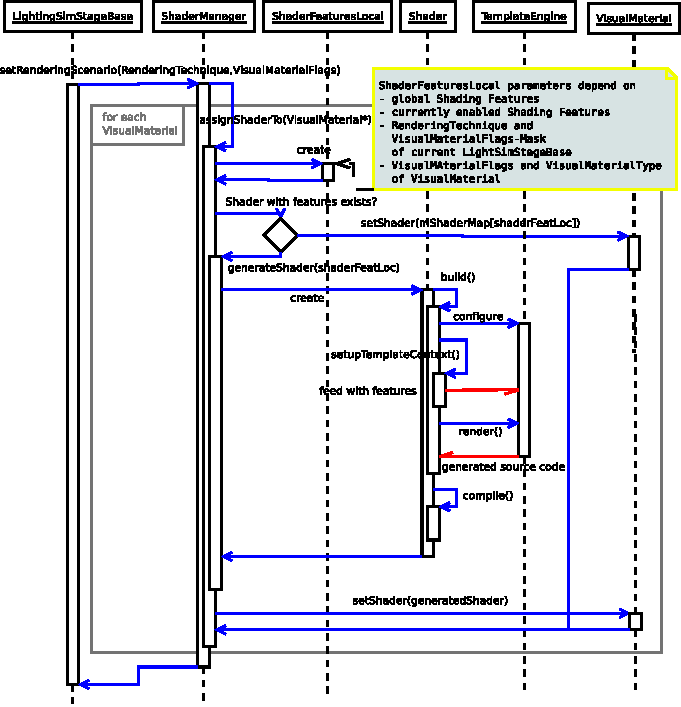
\includegraphics[width=1.09\textwidth]{ShaderGeneration.pdf}
	\caption{Sequenz-Diagramm der Shader-Generierung}
	\label{fig:shaderGen}
	\end{figure}
	
	Die Parameter sind:	
	\begin{description}
	
	
		\item[ShaderFeaturesGlobal] Parameter, die global per Config gesetzt wurden und ohne Reset der Engine nicht
			mehr zu ändern sind, und aufgrund von Buffergrößen, Kompatibilitäten und/oder der schlichten Konsitenz
			des visuellen Renderings sich zwischen den einzelnen Shadern nicht unterscheiden dürfen; dazu zählen:
		 	\begin{itemize}
		 	\item die maximale Anzahl an Lichtquellen
		 	\item die maximale Anzahl an Lichtquellen, die Schatten werfen (Shadow Caster),
		 	\item die maximale Anzahl an Instanzen, die pro Draw Call per Hardware Instancing gezeichnet werden kann
		 	\item falls man Deferred Rendering betreibt:
		 		 Der Textur-Typ des G-Buffers (\lstinline|Texture2D, Texture2DMultisample| etc.),
		 	\item falls man Deferred Rendering betreibt: Der MultiSample-Count des G-Buffers, falls er aus 
		 		MultiSample-Texturen besteht
		 	\item das
		 	\begin{lstlisting}
enum LightSourcesLightingFeature
{
	LIGHT_SOURCES_LIGHTING_FEATURE_NONE						=0,
	LIGHT_SOURCES_LIGHTING_FEATURE_ONE_SPOT_LIGHT			=1,
	LIGHT_SOURCES_LIGHTING_FEATURE_ONE_POINT_LIGHT			=2,
	LIGHT_SOURCES_LIGHTING_FEATURE_ALL_POINT_LIGHTS			=3,
	LIGHT_SOURCES_LIGHTING_FEATURE_ALL_SPOT_LIGHTS			=4,
	LIGHT_SOURCES_LIGHTING_FEATURE_ALL_POINT_OR_SPOT_LIGHTS	=5,
	__NUM_LIGHT_SOURCES_LIGHTING_FEATURES__					=6
}; 
		 	\end{lstlisting}
		 	Dieser Aufzählungstyp delegiert bei der Shader-Generierung per Template-Engine, welche Typen 
		 	und welche Anzahl an Lichtquellen vom Shader unterstützt werden sollen.
			\item das
		 	\begin{lstlisting}		 	
enum LightSourcesShadowFeature
{
	LIGHT_SOURCES_SHADOW_FEATURE_NONE			=0,
	LIGHT_SOURCES_SHADOW_FEATURE_ONE_SPOT_LIGHT	=1,
	LIGHT_SOURCES_SHADOW_FEATURE_ONE_POINT_LIGHT	=2,
	LIGHT_SOURCES_SHADOW_FEATURE_ALL_SPOT_LIGHTS	=3,
	__NUM_LIGHT_SOURCES_SHADOW_FEATURES__		=4
};	
		 	\end{lstlisting}
		 	Es gibt an, ob und wenn ja, welche Art Shadow Mapping vonstatten gehen soll.
		 	
		 	\item das
		 	\begin{lstlisting}
enum ShadowTechnique
{
	SHADOW_TECHNIQUE_NONE		=0,
	SHADOW_TECHNIQUE_DEFAULT	=1,
	SHADOW_TECHNIQUE_PCFSS		=2,
	__NUM_SHADOW_TECHNIQUES__	=3
};		 	
		 	\end{lstlisting}
		 	, welches bestimmt, nach welchem Algorithmus Shadowmapping vonstatten gehen soll
		\end{itemize}
		
		
		
		\item[diverse ShadingFeatures] 
		Diese Flags geben an, welche Shading-Features "`aktiv"' sind: Die \lstinline|ShadingFeatures| des letztendlich
		generierten Shaders hängen von den Shading Features des Materials selbst ab, aber auch von denen der 
		aktuell aktiven \lstinline|LightinSimStageBase| (eine \lstinline|ShadowMapGenerationStage| hat z.B. gar keine
		"`Shading"'-Features) und von den aktuell global aktivierten Features; Welche Features global aktiv sind, kann
		vom Benutzer bestimmt werden, hängt aber z.T. auch von der verwendeten OpenGL-Version ab; Tessellation kann z.B. 
		erst ab OpenGL 4.0 verwendet werden.
		
		\begin{lstlisting}
enum ShadingFeatures
	{
	SHADING_FEATURE_NONE				=1<<0,
	SHADING_FEATURE_DIRECT_LIGHTING		=1<<1,
	//global lighting via layered depth images or stuff... just a brainstroming, wont be implemented
	SHADING_FEATURE_GLOBAL_LIGHTING		=1<<2,
	SHADING_FEATURE_DIFFUSE_TEXTURING		=1<<3,
	SHADING_FEATURE_DETAIL_TEXTURING	=1<<4,
	SHADING_FEATURE_NORMAL_MAPPING		=1<<5,
	SHADING_FEATURE_CUBE_MAPPING		=1<<6,
	SHADING_FEATURE_AMBIENT_OCCLUSION	=1<<7,
	SHADING_FEATURE_TESSELATION			=1<<8,
	__NUM_SHADING_FEATURES__			=9
};
	\end{lstlisting}
		
		
	\item[VisualMaterialType]
	Der Typ bestimmt für gewöhnlich die Klasse des konkreten Shaders (erinnere: \lstinline|Shader| ist eine abstrakte 
	Basisklasse):	
	\begin{lstlisting}
enum VisualMaterialType
{
	VISUAL_MATERIAL_TYPE_NONE					=0,
	VISUAL_MATERIAL_TYPE_DEFAULT_LIGHTING  		=1,
	VISUAL_MATERIAL_TYPE_SKYDOME_RENDERING		=2,
	VISUAL_MATERIAL_TYPE_DEBUG_DRAW_ONLY		=3,	//just set a color value or something
	VISUAL_MATERIAL_TYPE_GAS_RENDERING			=4,
	VISUAL_MATERIAL_TYPE_LIQUID_RENDERING		=5,
	__NUM_VISUAL_MATERIAL_TYPES__				=6
};
	\end{lstlisting}
	
	
	\item[VisualMaterialFlags]
	Diese Klasse trägt nicht nur zur Delegation der Shader-Generierung bei, sie
	gibt auch bei einem \lstinline|VisualMaterial| bestimmte Eigenschaften an,
	welche auf Kompatibilität mit den Flags der aktuellen \lstinline|LightingSimStageBase| getestet werden können.
	Auf diese Weise können inkompatible Objekte masikert werden.
	Der Konstruktor reicht aus für eine Idee:
	\begin{lstlisting}
VisualMaterialFlags(
	bool castsShadows = true,
	bool isTransparent = false,
	bool isShadable = true,
	bool isDynamicCubeMapRenderable = true,
	bool isInstanced=false,
	bool isCustomMaterial=false);
	\end{lstlisting}
		
	\end{description}
	
	\sectionlevelfour{Probleme}
	Es sei noch ein nicht so unwichtiges Wort verloren über den Versuch, viele Effekte und Techniken in beliebiger
	Permutation zu kombinieren: Da dank der Template-Engine nun die Möglichkeit besteht, in Vererbungs-Hierachien zu denken
	und somit objektorientierte Ansätze ins Shader-Design einfließen zu lassen, zeigt sich umso krasser,
	wie schwer es ist, Effekte und Techniken sauber und modular zu kombinieren, wenn man obendrein noch maximale
	Performance haben will.\\
	Viele Features in einem Shader bringen bei Integration neue Einschränkungen mit sich, 
	die besonderer Behandlung bedürfen.
	Ein Beispiel ist die Kombination von Tessellation mit Shadow Mapping und/oder Layered Rendering: 
	Hier tut sich das Problem auf, dass wir zur Shadowmap-Generierung aus Sicht der Lichtquelle rendern 
	(die View-Matrix ist aus Position und Richtung der \emph{Lichtquelle} konstruiert), wir aber für Level-Of-Detail-	
	Berechnungen zur Bestimmung des Tessellation-Levels	Vertex-Positionen im \emph{Betrachter}-Viewspace benötigen!
	Dies hat den Grund, dass das LOD eines jeden Patches sowohl in der Shadow Map als auch im finalen Rendering
	gleich sein müssen! Wenn dies nämlich nicht der Fall ist, ist die Geometrie, die dem Shadow-Map-Lookup
	zugrunde liegt, eine andere als die des finalen Renderings; somit werden sprichwörtlich Äpfel mit Birnen verglichen,
	und es kann zu Artefakten kommen, z.B. Selbstverschattung, wo keine sein sollte (wenn durch Tessellation z.B.
	eine Furche generiert wird und die Lichtquelle weiter weg von der Geometrie ist als die Betrachter-Kamera, 
	s. Abb. \ref{fig:tessellationSelbstverschattung}).
	
	\begin{figure}[!h]
	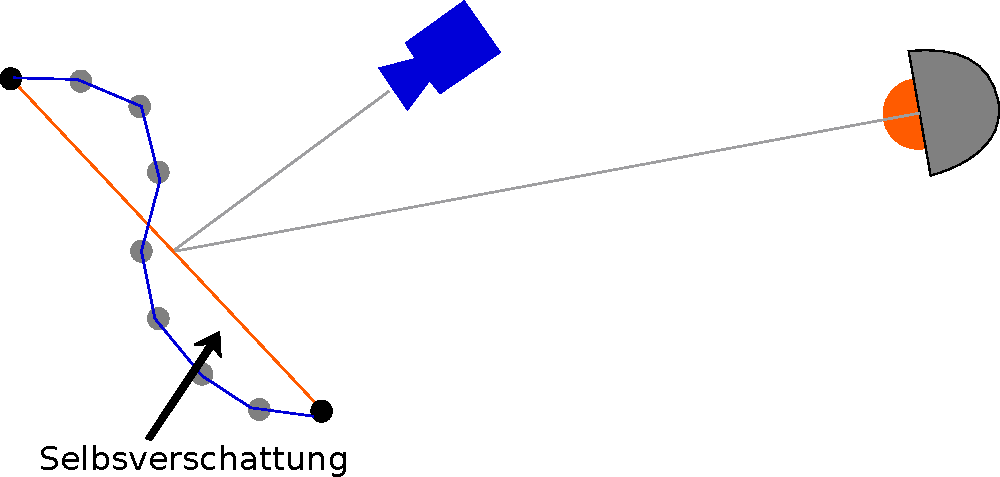
\includegraphics[width=\textwidth]{tessellationSelbstverschattung.pdf}
	\caption{Artefakte bei naiver Tessellation-Level-Berechnung mit Camera-Viewspace bei der Shadow Map Generation}
	\label{fig:tessellationSelbstverschattung}
	\end{figure}
	
	Um diese Artefakte zu vermeiden, muss für die LOD-Berechnung im Tesselation Control Shader
	\emph{immer} die Viewspace-Position der Vertices aus Sicht der Betrachter-Kamera zur Verfügung stehen.
	Bei der Shadow-Map-Generierung und/oder bei Layered Rendering (in Cube Maps und/oder Texture Arrays)
	werden aber für alles weitere, wie Displacement Mapping im Tessellation Evaluation Shader oder Beleuchtung
	im Fragment Shader, Viewspace-Positionen aus \emph{Lichtquellen}-Sicht bzw \emph{Worldspace}-Positionen durch die
	einzelnen Shader Stages geschleift.\footnote{bei Layered Rendering muss man bis zur Geomtry Shader Stage im 
	World Space (nur mit der Model Matrix) rechnen, da im Geometry Shader jedes Layer eine andere Kamera, also eine andere 
	View Matrix hat; Entsprechend kann  man keine ModelView Matrix für frühzeitige View Space-Berechnungen akkumulieren!}
	Somit sind die klassischen Interface-Varying-Veriablen schon belegt.
	Man muss also eine eine neue Variable benutzen, um die Betrachter-Kamera-View Space-transformierte Vertex-Position
	vom Vertex Shader an den Tessellation Control Shader zu übergeben. Da die built-in-Variable
	\lstinline[language=GLSL]|gl_Position| für OpenGL erst direkt vor der Fragment Shader-Stage für die Rasterisierung
	benötigt wird, kann man sie zuvor einfach zum Durchschleifen beliebiger Werte zweckentfremden. Somit ergibt sich
	folgender Vertex Shader Template-Code:
	\begin{lstlisting}[language=GLSL]
// step 2: calculate the gl_Position, if necessary 
 
  //default case:
  //we need projected transform for rasterization because no tessCtrl/TessEval/geom shader follows the vertex shader;
  gl_Position =  modelViewProjectionMatrix  * inVPosition; /*default MVP transform*/   
 
 
  
    //write the "spectator view space position" to gl_Position for tessellation LOD calculations 
    gl_Position =  spectatorCamViewMatrix * (modelMatrix * inVPosition);
  
    
      //write the "own view space position" to gl_Position for tessellation LOD calculations; 
      //Hence, even for dynamic cubemap generation, a modelViewMatrix must be passed 
      //to the vertex shader for this scenario;
      //The tessellation LOD calculation is invariant to cam rotation, 
      //hence only the translational part of the view matrix
      //is relevant, and this part is equal for every six cube map faces;
      gl_Position =  modelViewMatrix * inVPosition;
    
  

	\end{lstlisting}
	
	und für den Tesselation Control Shader:
	
	\begin{lstlisting}[language=GLSL]
//In order to determine the tessellation levels,
//we need all three vertex positions in spectator view space 
//of the triangle patch to which the current vertex belongs:

  //every user varyings are either in spectator world space
  //or in the light source- view- or world space;
  //but we need the VIEW space vertex positions seen from the SPECTATOR camera for the tessellation level calculations!
  //The vertex shader has written this value to gl_Position:
  vec3 edgeStart = gl_in[ (gl_InvocationID + 1) % 3 ].gl_Position.xyz;
  vec3 edgeEnd   = gl_in[ (gl_InvocationID + 2) % 3 ].gl_Position.xyz;
  vec3 ownVert   = gl_in[  gl_InvocationID          ].gl_Position.xyz;

  //no special case, we do just default rendering in spectator- view space; So grab the default position value:
  vec3 edgeStart = input[ (gl_InvocationID + 1) % 3 ].position.xyz;
  vec3 edgeEnd   = input[ (gl_InvocationID + 2) % 3 ].position.xyz;
  vec3 ownVert   = input[  gl_InvocationID          ].position.xyz;  
  
	\end{lstlisting}
	
	
	Das Fazit ist: Modulares Shader-Design, welches effizienten Code produziert, scheint je nach Feature-Set
	schwer bis unmöglich. Das Nutzen von Vererbungsmechanismen wird durch die notwendigen Spezial-Behandlungen 
	ebenfalls erschwert.
	Vor der Integration weiterer Features in diesen Uber Shader muss die Struktur überarbeitet werden.
	Ich war zur Zeit des Schreibens des Shader-Codes weder mit dem Templating vertraut, noch habe ich alle Spezialfälle
	antizipieren können. Ich hoffe, dass mit neuen Einsichten und Erfahrungen Les- und Erweiterbarkeit
	vom Shader-Code durch ein Refactoring verbessert können, und dass sich geeignete Wege finden, trotz Problemen wie dem
	vorgestellten Komplexität durch Vererbung besser zu handhaben.\\
	All diese Probleme betreffen nur den Shader-Code. Insbesondere die Vererbungsmechanismen
	lassen sich in OpenCL-Code-Templates reibungslos nutzen.


	%----------------------------------------------------------------------------------------------------------
		
	\subsubsection{CLProgram und CLProgramManager}
	\label{sec:CLProgram}
	
	\lstinline|CLProgram| und \lstinline|CLKernel| wrappen die entsprechende OpenCL-Funktionalität:
	Das Programm repräsentiert kompletten ausführbaren Code, welches aus einem in OpenCL C geschriebenen
	Source Code kompiliert wurde. Ein Kernel ist dagegen eine von womöglich mehreren Funktionen innerhalb
	des Programmms (durch das \lstinline[language=OpenCL]|__kernel|-Tag gekennzeichnet),
	welche vom Hostcode per \lstinline|cl::CommandQueue::enqueueNDRangeKernel()| aufgerufen werden kann.
	Es besteht also eine $1:n$-Relation zwischen Programm und Kernel.
	
	Die \lstinline|CLProgramManager|-Singleton-Klasse gewährleistet einen Zugriff auf sämtliche OpenCL-Programme
	im System über ihren Namen; Dies kann nützlich sein, wenn ein Kernel auf die Beendigung eines anderen Kernels
	warten muss, dafür das Event, was mit der letzten Ausführung assoziiert ist, benötigt, aber kein Handle auf die 
	entsprechenen \lstinline|CLProgram|s vorhanden ist.
	
	\lstinline|CLProgramManager| besitzt einen \lstinline|IntermediateResultBuffersManager|, der Buffers bereit stellt,
	die sich verschiedenen Kernels für ihre Zwischen-Ergebnisse teilen können. Somit wird GPU-Speicher gespart.
	Jedes \lstinline|CLProgram|, welches Kernels hat, die Zwischenergebnisse benötigen, kann eine bestimmte Menge
	und Größe an Buffers requesten. Es ist dann sichergestellt, dass der Buffer mit entsprechendem Index nach 
	Allokation (geschieht nach Erschaffung sämtlicher \lstinline|CLProgram|-Instanzen) mindestens die
	gewünschte Größe hat.
	 
	
		
		\sectionlevelfour{CLKernelArguments}
		\label{sec:CLKernelArguments}
		Der Umgang mit Kernel-Argumenten, also Parametern, die an die Kernel-Funktionen übergeben werden, 
		wird durch die Klasse \lstinline|CLKernelArguments| und seine Members deutlich erleichtert:
		In OpenCL kann man Werte an Kernels nur über ihren Index in der formalen Parameter-Liste übergeben.
		Diese holprige Methode ist nicht nur im Code wenig aussagekräftig, sie birgt auch die Gefahr,
		dass wenn Kernel-Signaturen sich ändern, im Host-Code genutzte Indices invalid werden.
		Wenn diese auch noch verteilt im System auftauchen, wird der Aufwand und die Fehlerwahrscheinlichkeit noch größer,
		seinen Host-Code anzupassen. Aus diesem Grund erstellt jedes konkrete CLProgram seine eigenen Kernels,
		und erstellt auch eine Liste an Default-Parametern für jeden Kernel. Auf diese Parameter kann nun bequem
		sowohl per Index als auch über den Namen des Arguments zugegriffen werden. Typsicherheit ist ebenfalls
		durch die Template-Klasse \lstinline|CLValueKernelArgument| gewährleistet, wo bei einem falschen
		Cast eine Exception geworfen wird.
		Ferner behebt das \lstinline|CLBufferKernelArgument| das bereits erwähnte Binding-Problem 
		beim Toggle von PingPong-Buffers.\\
		Ein detaillierteres Klassendiagramm zu den OpenCL-relevanten Klassen,
		welches zusätzlich die Call-Hierarchie des Build-Prozesses sowie einer Kernel-Invocation skizziert,
		zeigt Abb. \ref{fig:OCLRelatedClassDiag}.
		
		\begin{figure}[t]
		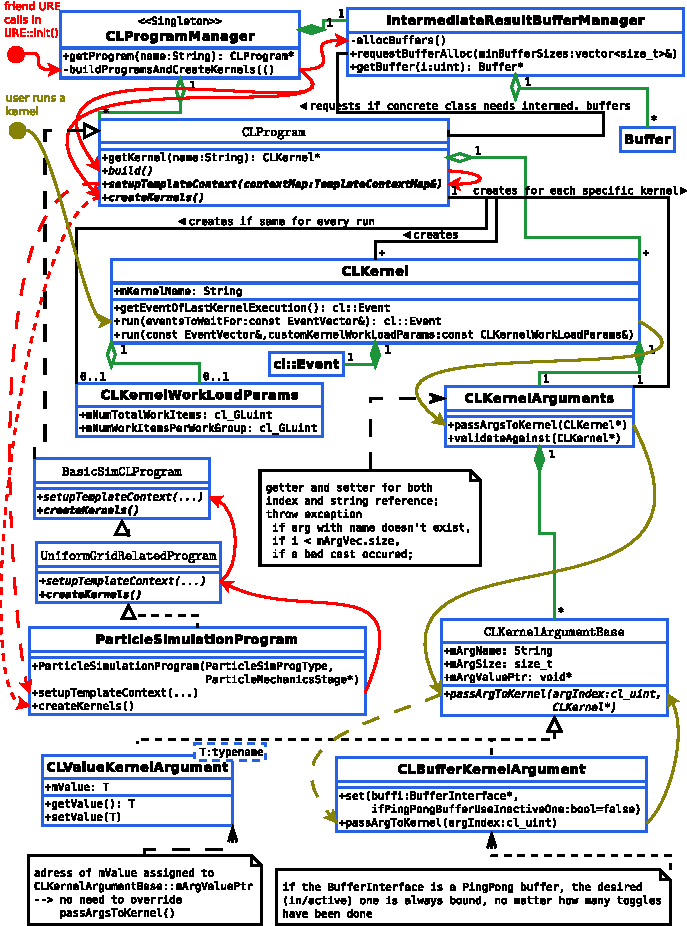
\includegraphics[width=\textwidth]{CLProgramAndCo.pdf}
		\caption{Klassendiagramm der OpenCL-relevanten Klassen inkl. Skizze der Call-Hierarchie des Build-Prozesses
		sowie dem Kernel-Launch}
		\label{fig:OCLRelatedClassDiag}
		\end{figure}



\subsection{Status der Implementierung am Ende der BA}
\label{sec:statusImplementation}

	Es sollten von Anfang an bei der Planung der \emph{Unified Engine} viele Aspekte berücksichtigt worden,
	damit von vornherein ein flexibles und mächtiges System konzipiert werden konnte.
	Das Potential zur Weiterentwicklung war wichtiger als eine "`schnell gehackte Demo"'.
	Es wurden einige Features realisiert, andere sind nahezu vollständig programmiert, aber noch nie ausgeführt worden
	\footnote{Mein Programmierstil ist sehr eigenwillig: ich kann wochenlang programmieren, 
	ohne einmal compilen, geschweige denn ausführen zu können. Dieser Stil scheint mir bei einem solchen Projekt nicht 
	völlig verkehrt, da bei der sukkessiven Entwickling der Fokus auf den Feature-Reichtum dem eines konsitenten 
	Gesamtsystems vorgezogen werden könnte.}. Widerum andere Fesatures liegen als Algorithmen in Textdateien herum, und 
	es ergab sich noch keine Gelegenheit, diese Algorithmen in Programm-Code zu transformieren.
	Wieder andere Features wurden nur ganz grob im Hinterkopf behalten, um die Wahrscheinlichkeit zu erhöhen, 
	dass sie in ferner Zukunft nahtlos mit den anderen Features integrierbar sind.\\
	Eine Liste dieser Features, mit ihrem entsprechenden Implementations-Status ist in 
	Tabelle \ref{tab:statusImpl1} und \ref{tab:statusImpl2} zu finden.\\
										  

 	\begin{table}[!h]
	 	\begin{minipage}{\textwidth}
  		\begin{tabular}
  		{
  		 l  l | c |
  		}
																	\cline{3-3}
  									&								&	Status \\ 
    	\noalign{\hrule}
    	%-------------------------------------------------------------------------------------------------
    	\multicolumn{1}{|c|}{
    		\multirow{3}{*}{used OpenGL Features}
    	}							& 	Uniform Buffers				&  {\color{green}\checkmark}		\\	
		\multicolumn{1}{|c|}{} 		& 	Instancing					&  {\color{green}\checkmark}
												\footnote{Transformation Matrix set provided per Uniform Buffers} \\	
		\multicolumn{1}{|c|}{} 		& 	Tessellation 
										\footnote{providing dynamic LOD, detail added via Displacement Mapping}
    																&  {\color{green}\checkmark}		\\	
		\noalign{\hrule}
		
    	%-------------------------------------------------------------------------------------------------
 		\multicolumn{1}{|c|}{
    		\multirow{3}{*}{Lighting}
    	}							& 	arbitrary light source amount in Shader	&  {\color{green}\checkmark} 
													    	\footnote{As long as they fit into an Uniform Buffer}	\\    	
    	\multicolumn{1}{|c|}{} 		& 	point light lighting		&  {\color{green}\checkmark}		\\	
    	\multicolumn{1}{|c|}{} 		& 	spot light lighting			&  {\color{green}\checkmark}		\\
    	\multicolumn{1}{|c|}{} 		& 	both point and spot light lighting	&  {\color{green}\checkmark}		\\   	
    	
    	\noalign{\hrule}
    	
    	%-------------------------------------------------------------------------------------------------					
    	\multicolumn{1}{|c|}{
    		\multirow{8}{*}{Deferred Rendering}
    	}							& 	Render to 2D Depth Texture		&  {\color{green}\checkmark}		\\				
		\multicolumn{1}{|c|}{} 		& 	Render to 2D Color Texture		&  {\color{orange}o}		\\		
		\multicolumn{1}{|c|}{} 		& 	Render to MultiSample  Color Texture		&  {\color{orange}o}		\\		
		\multicolumn{1}{|c|}{} 		& 	G-Buffer Fill				&  {\color{orange}o}		\\		
		\multicolumn{1}{|c|}{} 		& 	G-Buffer Shade				&  {\color{orange}o}		\\		
		\multicolumn{1}{|c|}{} 		& 	G-Buffer MultiSample Shade	&  {\color{orange}o}		\\		
		\multicolumn{1}{|c|}{} 		& 	Ambient Occlusion			&  {\color{red}x}		\\			
		\multicolumn{1}{|c|}{} 		& 	Post Processing \footnote{Participating Media, Depth Of Field etc.}	
																	&  {\color{red}x}		\\							
		\noalign{\hrule}
		
		%-------------------------------------------------------------------------------------------------					
		\multicolumn{1}{|c|}{
    		\multirow{4}{*}{Layered Rendering}
    	}							& 	Render to  Cube Depth Texture		&  {\color{orange}o}		\\		
    	\multicolumn{1}{|c|}{} 		& 	Render to  Cube Color Texture		&  {\color{darkred}o}		\\		
		\multicolumn{1}{|c|}{} 		& 	Render to  Depth Texture Array		&  {\color{orange}o}		\\
		\multicolumn{1}{|c|}{} 		& 	Render to  Cube Depth Texture Array		&  -
																	\footnote{only supported in OpenGL 4}\\
																	
		\noalign{\hrule}    	
    	
    	%-------------------------------------------------------------------------------------------------					
		\multicolumn{1}{|c|}{
    		\multirow{4}{*}{Shadow Mapping Support}
    	}							& 	single spot light					&  {\color{green}\checkmark}	\\		
		\multicolumn{1}{|c|}{} 		& 	single point light \footnote{requires render to  Cube Depth Texture}				
																			&  {\color{orange}o}		\\
		\multicolumn{1}{|c|}{} 		& 	multiple spot light \footnote{requires render to Depth Texture Array}				
																			&  {\color{orange}o}		\\
    	\multicolumn{1}{|c|}{} 		& 	multiple point light \footnote{requires render to Cube Depth Texture Array}																							&  -		\\
    				
		\noalign{\hrule}    	
    	
    	%-------------------------------------------------------------------------------------------------					
		\multicolumn{1}{|c|}{
    		\multirow{2}{*}{Shadow Map Sampling}
    	}							& 	default				&  {\color{green}\checkmark}	\\		
		\multicolumn{1}{|c|}{} 		& 	PCFSS				&  {\color{red}x}		\\
    															
																							
		\noalign{\hrule}
		
		%-------------------------------------------------------------------------------------------------					
		\multicolumn{1}{|c|}{
    		\multirow{6}{*}{misc. Shading Features}
    	}							& 	arbitrary (useful) effect combination	
    														&  {\color{green}\checkmark}	\\		
		\multicolumn{1}{|c|}{} 		& 	diffuse texturing	&  {\color{green}\checkmark}	\\	
		\multicolumn{1}{|c|}{} 		& 	detail texturing 
									\footnote{high frequency noise pattern to omit blurry appearance on close-up}
															&  {\color{red}x}	\\	
		\multicolumn{1}{|c|}{} 		& 	Normal Mapping		&  {\color{green}\checkmark}	\\	
		\multicolumn{1}{|c|}{} 		& 	Environment Mapping	&  {\color{green}\checkmark}	\\	
		\multicolumn{1}{|c|}{} 		& 	Sky Dome			&  {\color{green}\checkmark}	\\	
		\multicolumn{1}{|c|}{} 		& 	transparency		&  {\color{red}x}		\\
    																				
		\noalign{\hrule}

  		\end{tabular}	
  	
  		\caption{		
  			Status der Implementation zum Zeitpunkt der Abgabe der Ausarbeitung (englisch wegen vielen Fachbegriffen)
  			Legende: \\
			{\color{green}\checkmark}	$\rightarrow$ implementiert;
			{\color{orange}o}	$\rightarrow$ zu weiten Teilen programmiert, jedoch noch nicht 		
				integriert/ausgeführt/getestet;
			{\color{darkred}o} $\rightarrow$ detailliert Konzipiert, jedoch nicht programmiert;
			{\color{red}x}	$\rightarrow$ im System langfristig konzipiert, jedoch nicht programmiert;
			- $\rightarrow$ Unterstützung nicht geplant
			\\
		}
		\label{tab:statusImpl1}
		\end{minipage}
  	\end{table}

 	\begin{table}[!h]
	 	\begin{minipage}{\textwidth}
  		\begin{tabular}
  		{
  		 l  l | c |
  		}
																	\cline{3-3}
  									&								&	Status \\ 
    	\noalign{\hrule}
		
		%-------------------------------------------------------------------------------------------------			
		\multicolumn{1}{|c|}{
    		\multirow{6}{*}{mech. fluid simulation}
    	}							& 	basic efficient SPH mechanics
    									\footnote{see section \ref{sec:fluidSim:ablauf}}
    														&  {\color{green}\checkmark}	\\		
		\multicolumn{1}{|c|}{} 		& 	hardware dependent optimizations
										\footnote{see section \ref{sec:hardwareOptimizations} }
															&  {\color{green}\checkmark}	\\
		\multicolumn{1}{|c|}{} 		& 	algorithmic tricks \& optimizations 
										\footnote{integrate density computation into force kernel,
											less bandwidth consuming integration scheme, 
											see section \ref{sec:ausblick} }
															&  {\color{orange}o}	\\								
		\multicolumn{1}{|c|}{} 		& 	multiple fluids		&  {\color{orange}o}	\\	
		\multicolumn{1}{|c|}{} 		& 	particle Rigid Bodies
															&  {\color{orange}o}	\\	
		\multicolumn{1}{|c|}{} 		& 	static triangle collision mesh
															&  {\color{darkred}o}	\\															
		\noalign{\hrule}
		
		%-------------------------------------------------------------------------------------------------					
		\multicolumn{1}{|c|}{
    		\multirow{5}{*}{vis. fluid simulation 
    			\footnote{implementation of \cite{Green2009FluidRenderingCurvatureFlow} is planned}
    		} 
    	}							& 	debug draw			&  {\color{green}\checkmark}	\\		
		\multicolumn{1}{|c|}{} 		& 	curvature flow		&  {\color{red}x}	\\
		\multicolumn{1}{|c|}{} 		& 	perlin noise		&  {\color{red}x}	\\
		\multicolumn{1}{|c|}{} 		& 	foam rendering		&  {\color{red}x}	\\		
		\multicolumn{1}{|c|}{} 		& 	fresnel effect		&  {\color{red}x}	\\		    																																					
		\noalign{\hrule}
		
  		\end{tabular}	
  	
  		\caption{		
  			Status der Implementation zum Zeitpunkt der Abgabe der Ausarbeitung (Fortsetzung)
		}
		\label{tab:statusImpl2}
		\end{minipage}		
  	\end{table}
  	
  	
  	\begin{figure}[!h]
		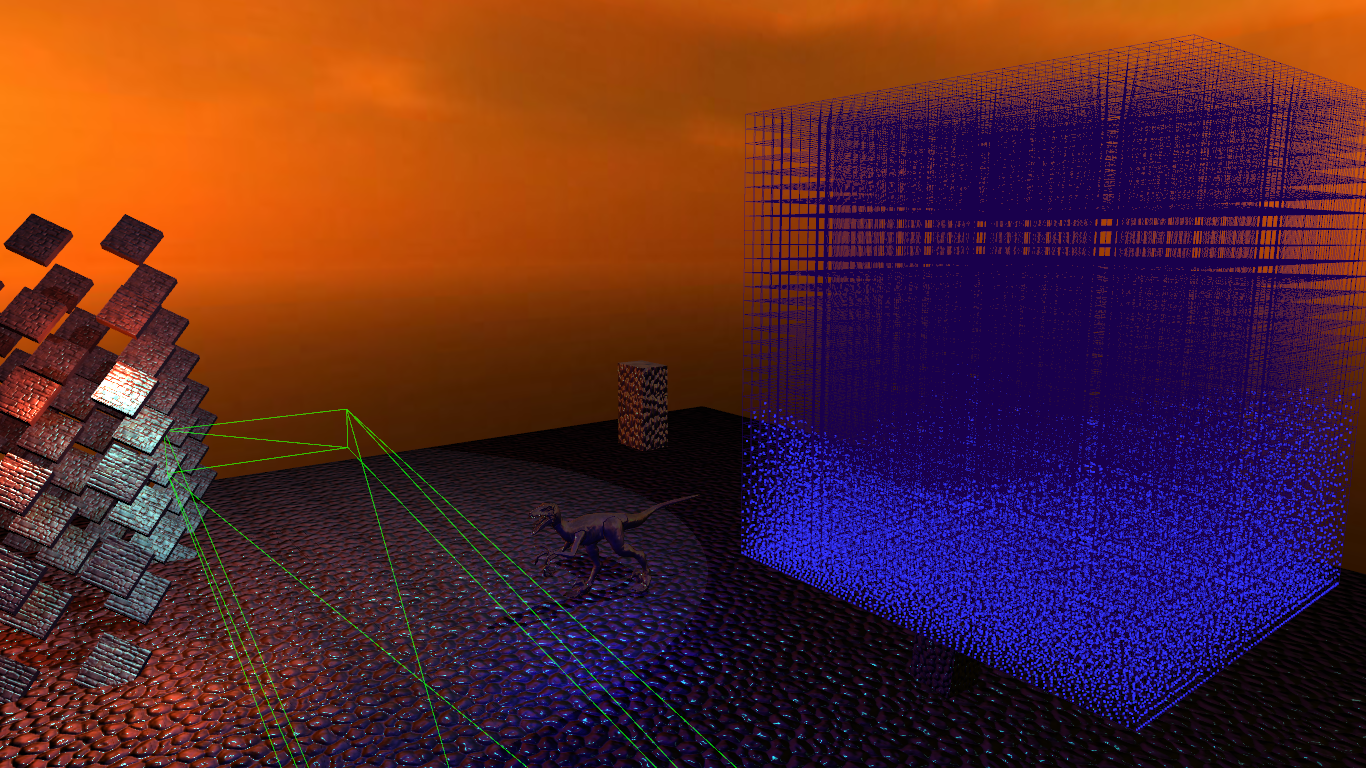
\includegraphics[width=1.3\textwidth]{Screenshot_prototypeSceneOverview.png}
		\caption{Überblick über die prototypische Szene}
		\label{fig:Screenshot_prototypeSceneOverview}
	\end{figure}
	
	Abb \ref{fig:Screenshot_prototypeSceneOverview} zeigt einen Screenshot aus \emph{Flewnit} 
	mit der prototypischen Scene. Sie zeigt die interaktive partikelbasierte
	Fluid-Simulation inklusive der Visualisierung des Uniform Grid, eine weitere Box mit 
	\linebreak \lstinline|DebugDrawMaterial|,
	einen Würfel aus Objekten, die per Instancing gezeichnet werden, tesseliert und normal mapped sind,
	einen Sky Dome, und schließlich ein tesselliertes, normal und environment mapped Raptor-Modell.
	Alle Objekte sind mit meheren Lichtquellen, sowohl Spot als auch Point Light, in einem Render-Pass beleuchtet.
	Ein Spot Light wirft per Shadow Mapping Schatten.  
	Details werden im Verlauf des Abschnitts \ref{sec:simulation} erläutert.\\
  	
  	Der größte Wermutstropfen bei der Implementierung ist sicherlich die Visualisierung des Fluids, die minimalistischer
  	technisch nicht sein könnte. Die Mechanik der Fluidsimulation stand erst wenige Wochen vor der 
  	Abgabe (die ersten Monate waren rein der Framework-Programmierung und dem nicht-Fluid-bezogenen
  	visuellen Rendering gewidmet), 
  	so dass für eine angemessene Visualisierung des Fluids im Rahmen dieser Arbeit leider keine Zeit mehr blieb.
  	Ich wollte schließlich meiner "`ganz oder gar nicht"'-Linie in diesem System treu bleiben, und werde die Visualiserung
  	ohne "`Zwischenlösung"' direkt implementieren, sobald Zeit ist. Hierfür möchte ich die in
  	"`Screen Space Fluid Rendering with Curvature Flow"' (\cite{Green2009FluidRenderingCurvatureFlow})
  	vorgestellte Lösung nach-implementieren.
  	
  	Weiterhin fehlen noch sämtliche erweiterten Features und "`a posteriori"'-Optimierungen (also Optimierungen, die 
  	nach der erfolgreichen ersten Implementierung programmiert sind) bei der mechanischen Fluid-Simulation.
  	Der Kernel- und Host-Code für die partikel-basierten Rigid Bodies ist fast komplett programmiert,
  	da der Beginn der Ausarbeitung aber sehr dringend wurde, habe ich der Versuchung wiederstanden,
  	diesen Code noch zu testen.\\
  	Weiterhin wollte ich "`static triangle collision meshes"' in die ansonsten partikelbasierte
  	mechanische Simulation integrieren, über den Entwurf eines
  	Algorithmus zur Voxelisierung von Dreiecken ins Uniform Grid bin ich jedoch nicht hinaus gekommen 
  	(mehr dazu im Ausblick, Kapitel \ref{sec:ausblick}).
  

  	Ferner habe ich zwar einen Scene-Loader mithilfe von \emph{Assimp} implementiert, es ist aber noch vieles
  	hart-Codiert, so dass das Laden von beliebigen Assets noch nicht möglich ist. Mein Fokus lag
  	auf der Realisierung von kombinierbaren Effekten, vorerst nicht auf künstlerischem Anspruch. 
  	Dennoch ist die Fertigstellung des Scene Loaders geplant.
	
	Die fehlende GUI erschwert das Parameter-Tweaken, was zur Zeit noch per XML-Datei geschehen muss.
	
	Für weitere Details im Umgang mit fehlenden Features und unvöllständiger Implementation sei auf
	den Ausblick in Abschnitt \ref{sec:ausblick} verwiesen.

\clearpage

	
\section{Simulation}
	\subsection{Die visuelle Simulationsdomäne}
		
\label{sec:visualDomain}
	
Ein paar worte ueber die shading features, wie sie maskiert werden, SceneNodeVisitor etc..

\subsubsection{Der LightingSimulator}
	Nochmal drauf hinweisen, dass Rendering etwas generisches in diesem Framework ist, und wir lieber von Lichtsimulation sprechen sollten, auch wenn es monetan nicht photrealistisch ist ;)

\subsubsection{Die Lighting Simulation Pipeline Stages}
	baseclass etc...
	shadowmap gen stage, direct lighting stage, was noch in planung is etc..

	in planung: deferred rendering G-Bufferfill, deferred rendering shade, div. post processing stages
	
\subsubsection{VisualMaterial}
	\label{sec:visualMaterial}
	
\subsubsection{Camera}


\subsubsection{LightSource und LightSourceManager}
	
	
\subsubsection{RenderTarget}	
	

\subsubsection{ShaderManager}
	generiert mit grantlee, assigned an materials und verwaltet Shader , abhaenging von der aktuellen lighting stage, den registierten Materials,
	der Erzeugten kontext, den vom user aktivierten rendering features etc pp

\subsubsection{genutzte moderne OpenGL- Features}	
	\label{sec:usedOpenGLfeatures}

	\paragraph{Hintergrund:Batching}
	PCIe-Bandbreite und -Latenz nicht überlasten durch immediate mode oder andere befehls-serien;
	\todo[color=green]{referenz zu PCIe-Flaschenhals-stuff}

	\paragraph{Uniform Buffers}
	auch von BufferInterface abstrahiert, vorteile auflisten, aber auch stolperfallen: alignment etc)	
	nutzen für transformationsmatrizen beim instancing und für beliebige lichtquekken

	
	\paragraph{Instancing}
	\label{sec:instancing}
	InstanManager, InstangedGeometry vorstellen, konzept, wie es verwaltet wird, erklaeren;
	batching
 	\lstset{language=GLSL}
 	\begin{lstlisting}[caption={Transformationsmatrizen-Uniforms im Vertex Shader},label=listing:VertShaderTransformDef]


  struct InstanceTransform
  {
    mat4 modelMatrix;  //needed for layered rendering to be combined with the several lightsource matrices
    mat4 modelViewMatrix; //needed in a non-layered context for calculation of view-space values for lighting calculations
    mat4 modelViewProjectionMatrix; //needed in a non-layered context for gl_Position calculation
    
    int uniqueInstanceID; //it is not guearnteed that for each "logic" instance, the gl_InstanceID stays the same for every draw call
                          //e.g. because of culling of "previous" instances, the own gl_InstanceID will get smaller 
    
    //no padding, because the offsets will be queried via glGetActiveUniformsiv(...)
  };

  layout(shared) uniform InstanceTransformBuffer
  {
    InstanceTransform instanceTransforms[  {{numMaxInstancesRenderable}} ];
  };

  uniform mat4 modelMatrix;
  uniform mat4 modelViewMatrix;
  uniform mat4 modelViewProjectionMatrix; 

 	\end{lstlisting}
 	\lstset{language=C++} %we want C++ code listings	
	
	
	
	\paragraph{Hardware Tesselation}
	basics des GL4- hardware features erwaehnen fuer den geneigten leser, raptor-modell erwaehnen und seinen 		
	Aufbereitungsprozess, LOD, displacement mapping erlaeutern	
	
	
\subsubsection{Ablauf}	

	
\subsubsection{Implementierte Effekte}
	\label{sec:genericVisualEffects}
%%-------------------------------------------------------------------------------------------------------
\todo[color=green]{diesen klumbatsch in form bringen, mit bildern anreichern etc pp}

Zunächst zum Begriff "Mapping", der so oft auftaucht: Englisch "map"-"Landkarte", "to map"-"abbilden" Bedeutet in der Computergrafik meist die Abbildung eines Bildes auf eine Oberfläche nach einem bestimmten Algorithmus;

- Beleuchtung durch beliebig viele Punkt- und Spot-Lichtquellen (also Lichtquellen mit eineme gerichteten Kegel, Scheinwerfer)

- Shadow Mapping: Erzeugen eines bildes aus Tiefenwerten, anschließend vergleich der Tiefenwerte aus Kamerasicht mit denen aus Lichtquellensicht (der "shadow map", Schattenkarte), pixel im finalen Bild gilt als verdeckt wenn Tiefenwert aus Kamerasicht größer als der entsprechende Pixel in der shadow map, unverdeckt wenn nicht;

- Normal Mapping: Verzerrung der Oberflächen-Normalen (Vektor Sekrecht zur Oberfläche) um relief-artige Geometriedetails zu simulieren, ohne dass tatsächlich diese feine Geometrie in der virtuellen Szene existiert; Dies spart Rechenleistung und Speicher im Vergelcih zu einer Szene, wo all dieses Detail tatächlich in der Geometrie vorhanden wäre; Anschauliches Anwendungsbeispiel: Illusion der feinen Geometrie von Rauhfasertapete auf einem schlichten Quadrat; Nachteil: Die geometrische Illusion brich bei flachen Betrachtungswinkeln ein, die Flachheit der eigentlichen, simplen Geometrie fällt dann auf; Die Information der verzerrten Normalen stammt ebenfall aus einem Bild, der "normal map"; Diesmal werden die Pixelwerte jedoch nicht als Farben oder Tiefenwerte, sondern als Abweichung von der unverzerrten Normalen interpretiert (rot->x-Achse;grün->y-Achse; blau->z-Achse); Da im Computer alles nur Zahlen sind und Semantik erst durch unsere Verwendung und Wahrnehmung erlangen, und da die Graphikkarten so weit flexibel/programmierbar geworden sind, dass man als Programmierer Kontrolle über derartige "Um-Interpretierung" hat, ist dies möglich;

- Environment mapping: Der Trick, perfekt spiegelnde Materialen vorzugaukeln: Es wird in einer "Cube map" nachgeschaut, einer Sammlung von sechs bildern, wo jedes Bild eine Würfelseite repräsentiert; Die Reichtung der Normalen eines Pixels wird umgerechnet in eine Koordinaten, mit der in der Cube Map nachgeschaut wird; Dieser Frabwert fießt dann in die Farbe des Pixels des finalen Bildes ein; Vorteil: Dinge wie lackierte Autokarosserien lassen sich ganz gut vorgaukeln, mit recht geringem Rechenaufwand; Nachteil: Da für gewöhnlich nur in einem statischen Bild nachgeschaut wird, können dynamische Änderungen der Szene bei der "pseudo-spiegelung" nicht erfasst werden; Ein Objekt, welches sich nache eines autos bewegt, bewegt sich ein seiner "Spiegelung" nicht; Aus solchen Gründen sind in Cube maps oft nur sehr entfernte Dinge dargestellt: Horizong, Himmel, Wolken etc.; Diese Dinge ändern sich in der Realistät ja nicht so schnell, daher fällt der Nachteil beim environment mapping unter dieser Einschränkung nicht mehr so drastisch auf; Der Hintergrund, die orangene Dämmerung, ist gnau diese Cube map, die ich also sowohl für die Pseudo-Spiegelung als auch als "Füllmaterial" dort, wo ich keine Geometrie in der Szene habe, verwende;

- Tesselation: Wie Bei Normal Mapping soll der wahrgenommene Detailgrad der Geometrie erhöht werden; Jedoch erzeugt die Tesselation "`echte"' Geometrie, in Abhängigkeit von der Entwerfnung eines Objekte zur Betracher-Kamera; Somit wird dort Geometrie erzeugt, wo sie nötig für den Detailgrad des aktuellen Bildes ist, und dort eingespart, wo sie momentan unnötig ist; Diese Technik hat nicht die Nachteile des Normal mappings; Jedoch Ist durch die Reine Erzeugung von Geometrie noch nicht viel gewonnen; Sinn bekommt diese neue  Geometrie wert dann, wenn sich auch wirklich mehr Datail mit ihr darstellen lässt; Erreicht wird dies durch eine sogenannte Displacement Map (frei Übersetzt "Verschiebungs-Karte", ein Bild, in dem Tiefenwerte der Hoch-detaillierten Geometrie gepeichert sind). Die neu erzeugte Geometrie wird also entlang der Normalen um den Betrag verschoben, wie in der Displacement Map eingetragen ist; Somit entsteht ein "tatsächliches Relief", im gegensatz zum Vorgegaukelten Relief beim Normal Mapping; MEhr Details erspare ich dir, z.b. Warum man Normal Mapping trotzdem immer noch für die Beleuchtung braucht, trotz der Tesselation und dem Displacement mapping;

Anmerkung: Weil ich Tesselation so toll finde, habe ich mir das Velociraptor-3D-Modell aus dem Internet besorgt; Dieses hatte 5 Milloonen Dreiecke; Ich habe es mit einem Programm (was ich nicht selbst geschrieben habe, davon versteh ich leider noch viel zu wenig) herunterrechnen lassen, so  dass ein vereinfachtes Modell mit etwa 11000 Dreicken entstand, also ein etwa zweitausend mal simpleres Modell. Mit einem anderen Programm habe ich dann die Geometrie des komplexen Modells auf die des simplen Modells projeziert, die detailgrad-bedingte Distanz zwischen den Geometrien in ein Bild geschrieben; Dieses Bild ist die Displacement map für die Tesselation izur Darstellung in meinem eigenen Programm; Somit kann ich nun den Dinosaurier beinahe so detailliert darstellen, wir er im Originalmodell vorliegt, jedoch mit viel höheren Bildwiederholungsraten; 

%%-------------------------------------------------------------------------------------------------------
	  

\clearpage
	
	\subsection{Die mechanische Simulationsdomäne}
		
\subsection{Die Meachanische Domäne}
{sec:mechanicalDomain}


\clearpage



\section{Ergebnisse}

	

\begin{figure}[!h]

	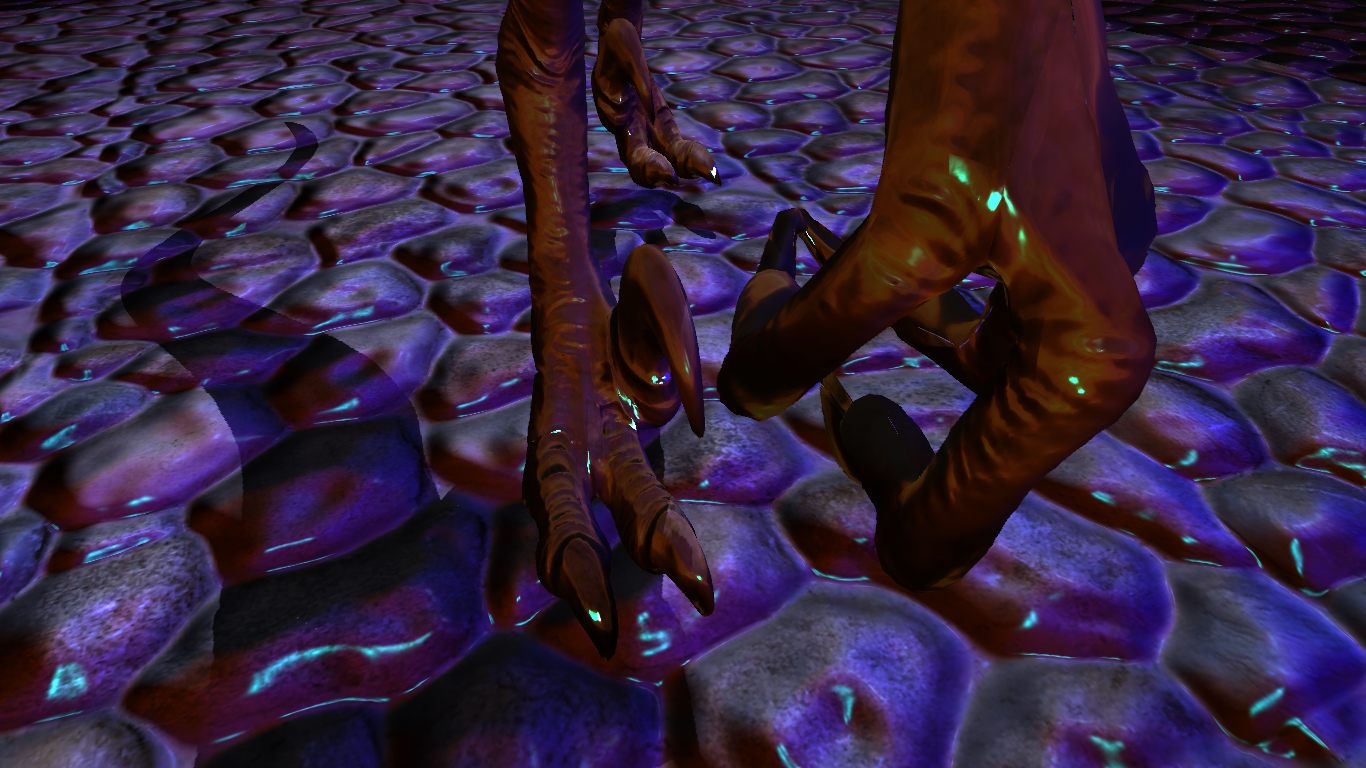
\includegraphics[width=1.2\textwidth]{Screenshot_raptorExtremities_allFX.png} 
	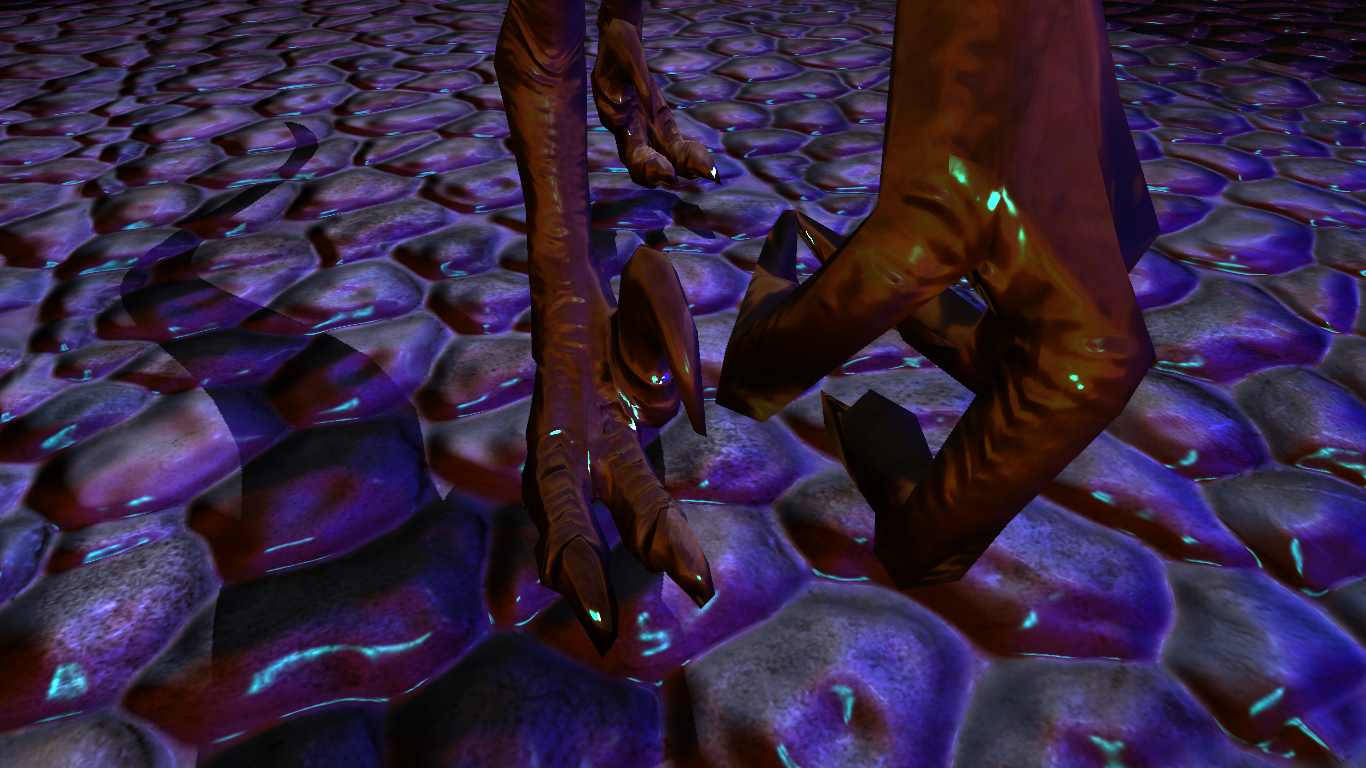
\includegraphics[width=1.2\textwidth]{Screenshot_raptorExtremities_allFX_withoutTess.png}

	\caption{Die Extremitäten des Raptor-modells; Oben: tesseliert, texturiert, normal mapped, environment mapped, 
	beleuchtet von fünf Lichtquellen , shadow mapped von einer Lichtquelle; Unten: wie oben, nur ohne Tessellation
	}
	\label{fig:shaderfeaturePermutations}
\end{figure}


\begin{figure}[!h]	 	
	\begin{tabular}{ x{0.5\textwidth} x{0.5\textwidth} }
		
		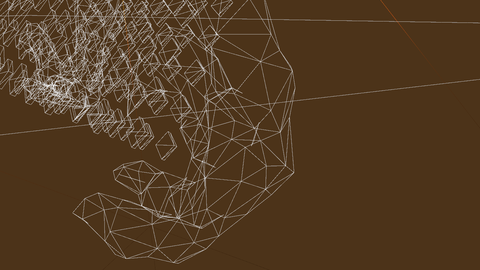
\includegraphics[width=0.5\textwidth]{resized/resized_Screenshot_raptorClaws_pure_WIRE.png} 
		wire frame	
		&
		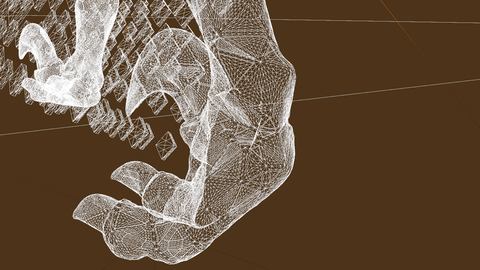
\includegraphics[width=0.5\textwidth]{resized/resized_Screenshot_raptorClaws_pure_WIRE_tess.png} 
		wire frame, tessellated
		\tabularnewline

		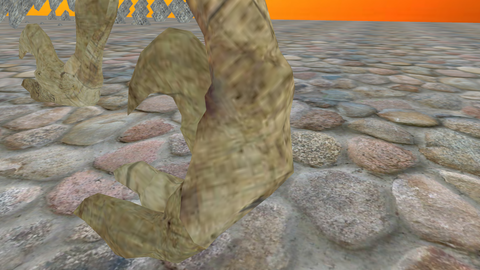
\includegraphics[width=0.5\textwidth]{resized/resized_Screenshot_raptorClaws_diffuseTex.png} 
		diffuse textured
		&
		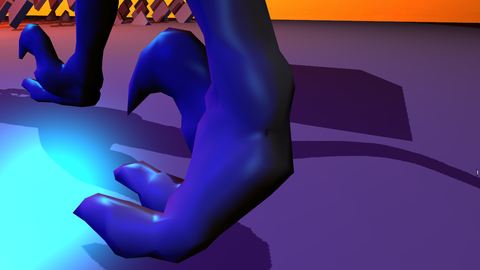
\includegraphics[width=0.5\textwidth]{resized/resized_Screenshot_raptorClaws_lighting.png}
		lighted
		\tabularnewline
		
		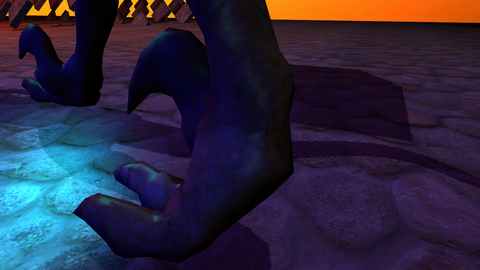
\includegraphics[width=0.5\textwidth]{resized/resized_Screenshot_raptorClaws_lighting_diffuseTex.png} 	
		lighted, diffuse textured
		&
		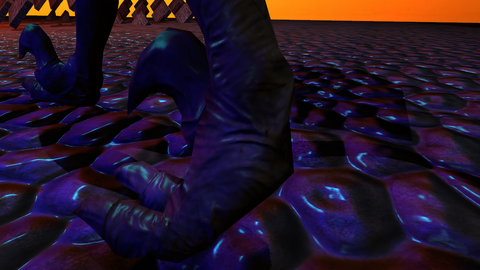
\includegraphics[width=0.5\textwidth]{resized/resized_Screenshot_raptorClaws_lighting_diffuseTex_normalMap.png}	
		lighted, diffuse textured, normal mapped
		\tabularnewline

		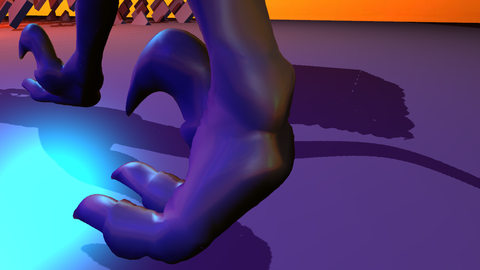
\includegraphics[width=0.5\textwidth]{resized/resized_Screenshot_raptorClaws_lighting_envmap_tess.png} 	
		lighted, diffuse textured, environment mapped, tessellated
		&
		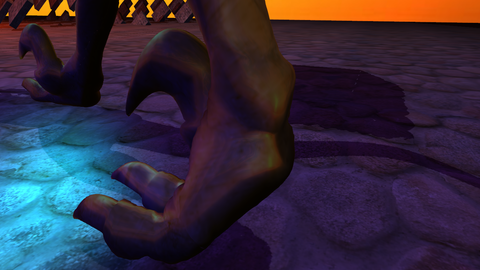
\includegraphics[width=0.5\textwidth]{resized/resized_Screenshot_raptorClaws_lighting_diffuseTex_envmap_tess.png}
		lighted, diffuse textured, environment mapped, tessellated
		\tabularnewline		
		
		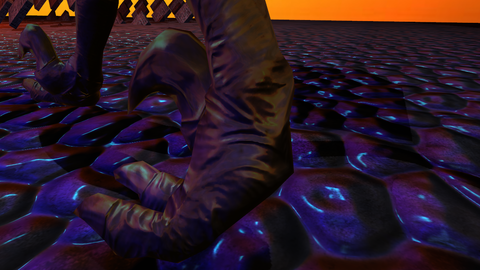
\includegraphics[width=0.5\textwidth]
			{resized/resized_Screenshot_raptorClaws_lighting_diffuseTex_normalMap_envMap.png} 	
		lighted, diffuse textured, normal mapped, environment mapped
		&
		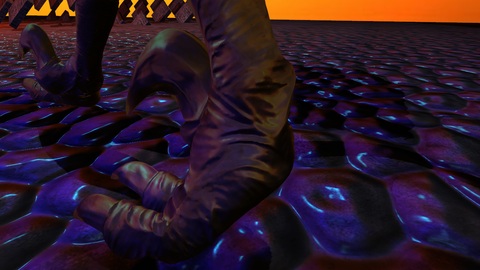
\includegraphics[width=0.5\textwidth]
			{resized/resized_Screenshot_raptorClaws_lighting_diffuseTex_normalMap_envMap_tess.png}		
		lighted, diffuse textured, normal mapped, environment mapped, tessellated
		\tabularnewline
	\end{tabular}
	\caption{Füße des Raptor-Modells, mit verschiedenen Permutationen aktivierter Shader-Features}
	\label{fig:shaderfeaturePermutations}
\end{figure}




\begin{figure}[!h]	 	
	\begin{tabular}{ x{0.5\textwidth} x{0.5\textwidth} }

   		\multicolumn{2}{ x{\textwidth} }{   			
    			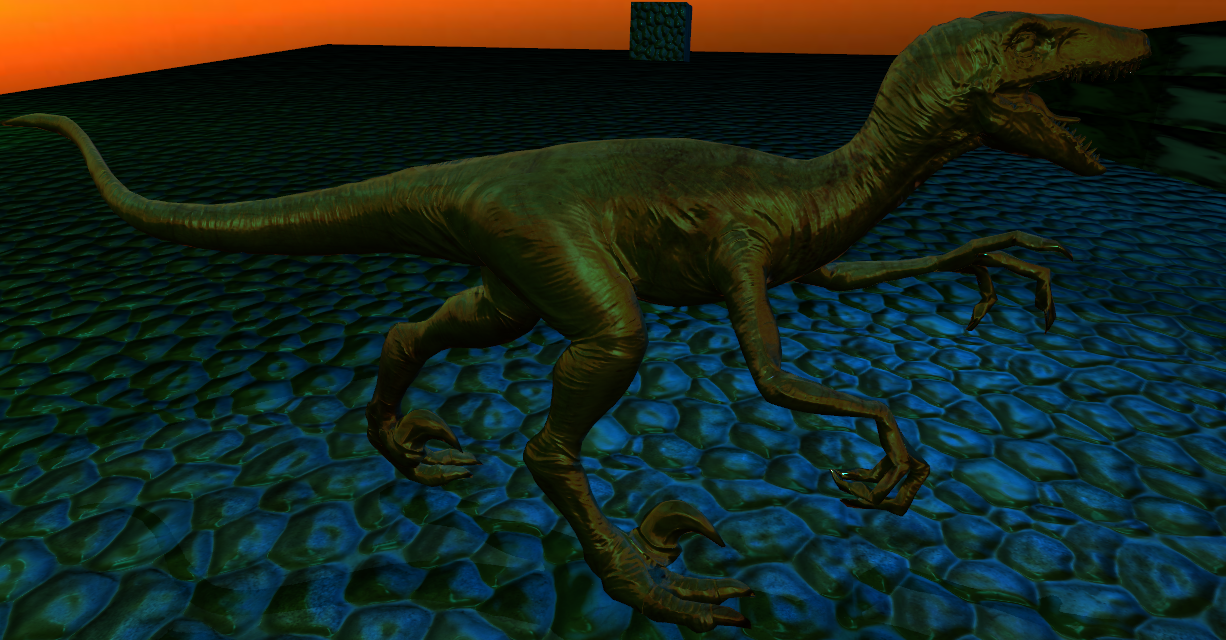
\includegraphics[width=\textwidth]{Screenshot_raptor_full.png} 
   		}	
   		\tabularnewline	
   		
   		\multicolumn{2}{ x{\textwidth} }{
    			Auf die Entfernung reicht das Normal Mapping noch aus,
		}
		\tabularnewline   		
		\multicolumn{2}{ x{\textwidth} }{
    			um Geometrie-Detail zu suggerieren ...
		}
		\tabularnewline
		
		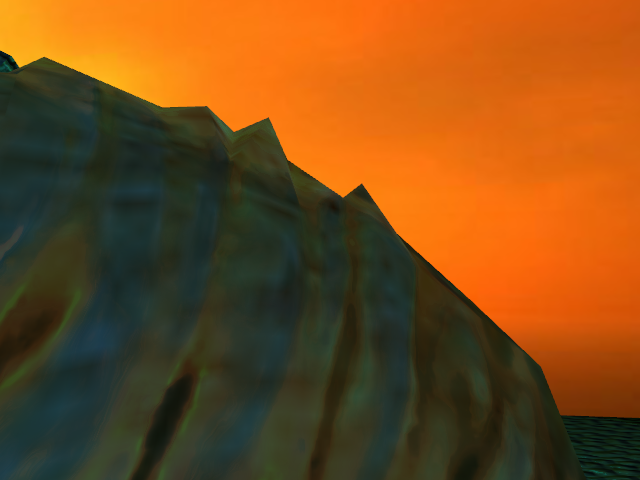
\includegraphics[width=0.4\textwidth]{Screenshot_raptorNeck_normal.png} 
		&
		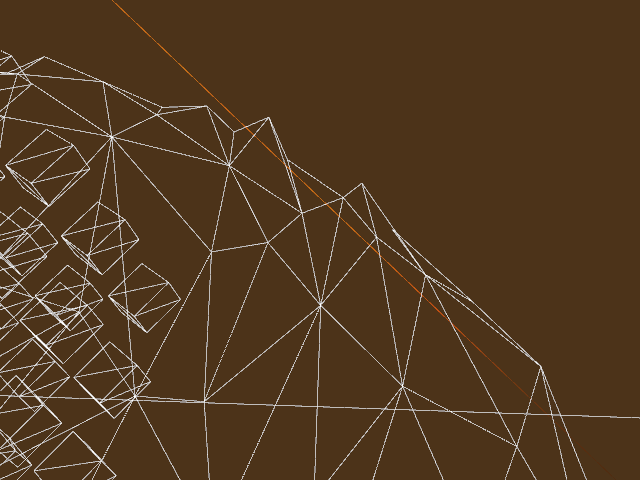
\includegraphics[width=0.4\textwidth]{Screenshot_raptorNeck_WIRE.png} 
		\tabularnewline
		
		\multicolumn{2}{ x{\textwidth} }{
			\multirow{1}{*}{
			... hier jedoch nicht mehr
			}
		}
		\tabularnewline
		
		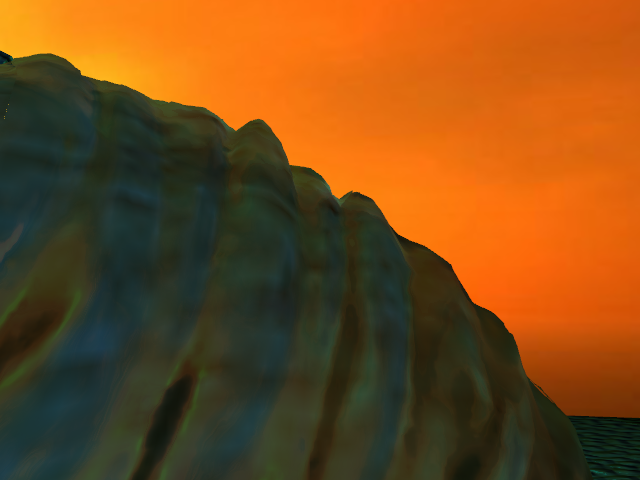
\includegraphics[width=0.4\textwidth]{Screenshot_raptorNeck_normaltess.png}
		&
		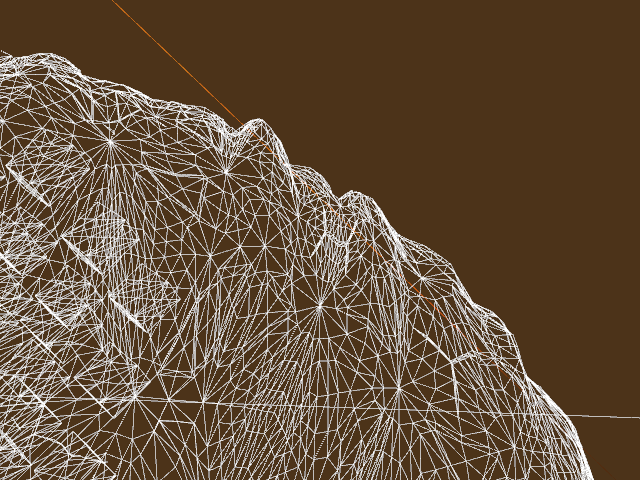
\includegraphics[width=0.4\textwidth]{Screenshot_raptorNeck_WIRE_tess.png}
		\tabularnewline

		%------------------------------------------------------------------------------
			
		%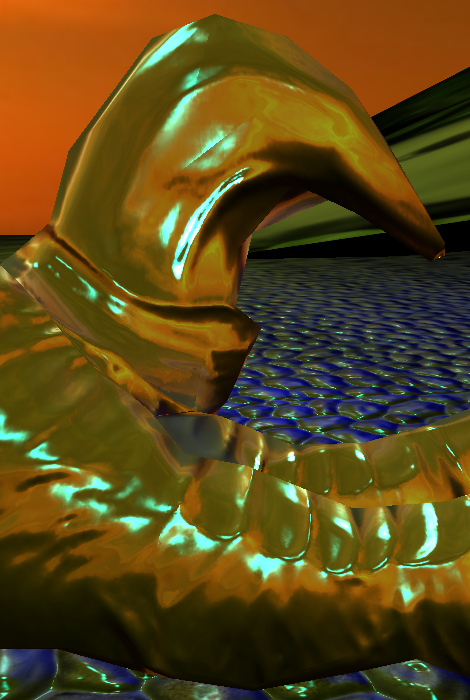
\includegraphics[width=0.4\textwidth]{Screenshot_raptorFootCloseUp_nonTess.png}
		%&
		%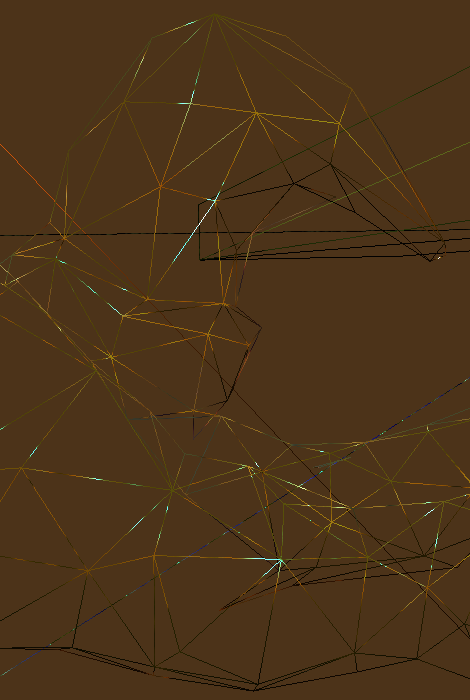
\includegraphics[width=0.4\textwidth]{Screenshot_raptorFootCloseUp_WIRE_nonTess.png}
		%\tabularnewline
		
		%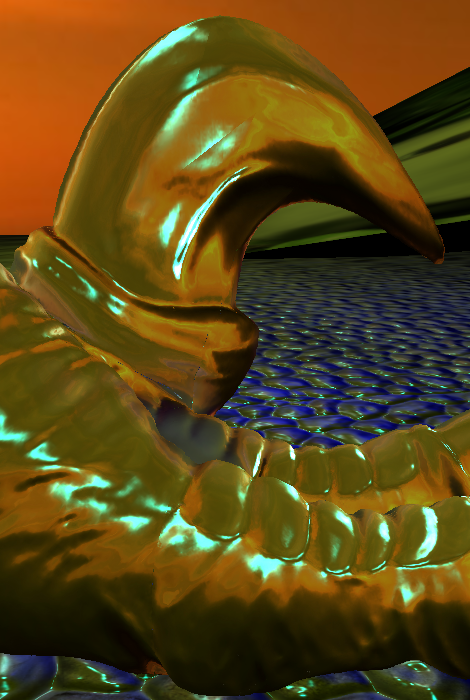
\includegraphics[width=0.4\textwidth]{Screenshot_raptorFootCloseUp_tess.png}
		%&
		%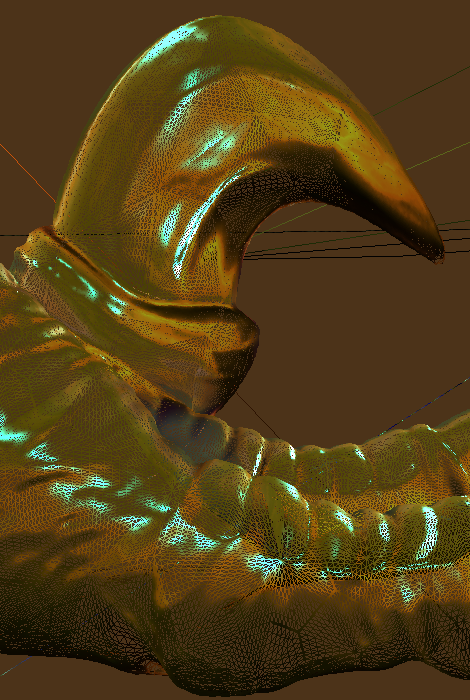
\includegraphics[width=0.4\textwidth]{Screenshot_raptorFootCloseUp_WIRE_tess.png}
		%\tabularnewline

	\end{tabular}
	\caption{Gegenüberstellung des Detail-Grades mit und ohne Tessellation, Teil 1}
	\label{fig:sefef}
\end{figure}

\begin{figure}[!h]	 	
	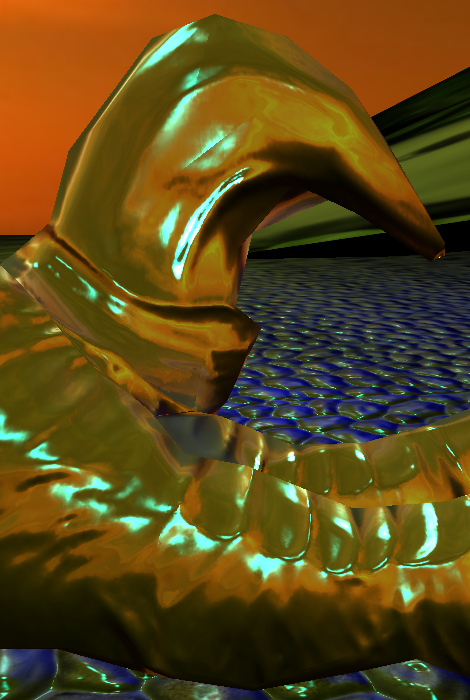
\includegraphics[width=0.5\textwidth]{Screenshot_raptorFootCloseUp_nonTess.png} 
	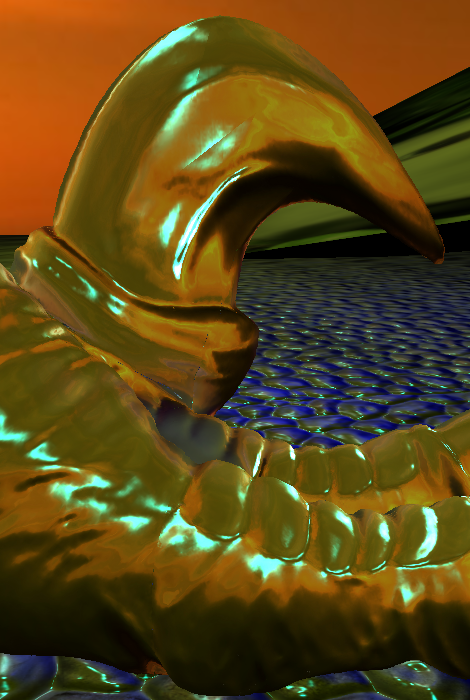
\includegraphics[width=0.5\textwidth]{Screenshot_raptorFootCloseUp_tess.png} 
	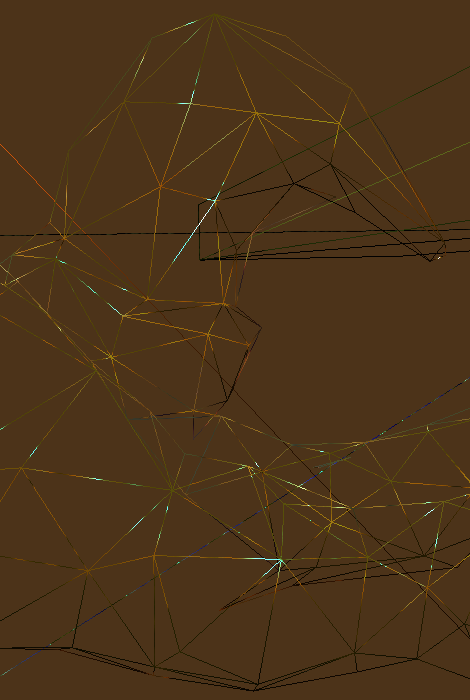
\includegraphics[width=0.5\textwidth]{Screenshot_raptorFootCloseUp_WIRE_nonTess.png} 
	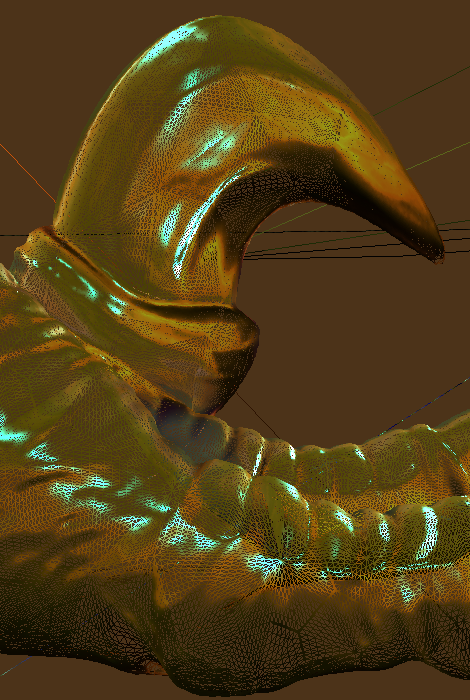
\includegraphics[width=0.5\textwidth]{Screenshot_raptorFootCloseUp_WIRE_tess.png} 

	\caption{Gegenüberstellung des Detail-Grades mit und ohne Tessellation, Teil 2}
	\label{fig:gegenueberstellungTessNonTess}
\end{figure}




\clearpage


\section{Ausblick}

	



	Zunächst möchte ich ergänzende Information zu dem Ansatz und der Motivation der
	"`static triangle collision meshes"' liefern, die in Abschnitt \ref{sec:statusImplementation} 
	angedeutet wurden:\\
  	Mich hat es schon während der Recherche-Phase gestört, dass ich keine Information gefunden habe, ob und wenn ja, 
  	wie primitiv-basierte Rigid Body-Simulation -- also eine Simulation, wo die Rigid Bodies 
  	aus Dreiecken oder komplexeren Primitiven aufgebaut sind und nicht aus Partikeln --
  	auf der GPU effizient möglich ist. Ich habe nur Papers
  	zu CPU/GPU-hybriden Ansätzen oder partikel-repräsentierten Rigid Bodies gefunden (letzteren Ansatz
  	habe ich selber in meinem ungetesteten Code verwendet). 
  	Ich wollte zumindest für statische Dreiecks-Meshes testen, ob diese,
  	da sich ihre räumliche Position und damit auch die Postion im Speicher nicht mehr ändert,
  	effizient auf die GPU zu mappen sind. Hierfür habe ich einen Algorithmus entwickelt, der beschreibt,
  	wie man das Mesh überhaupt erst einmal Artefakt-frei aufbereitet für die Integration in ein Uniform Grid 
  	(über Voxelisierung von	Primitive- ID's, wobei der Umstand zu berücksichtigen ist, 
  	dass ein Vertex zu beliebig vielen Dreiecken gehören kann).
  	Die nächste Herausforderung, wenn die Primitive-ID's wie Particle-ID's über das Uniform Grid verfügbar sind,
  	ist die Datenstruktur für die Dreiecke und eine effiziente Kollisions-Berechnung zwischen Dreick und Partikel.
  	Hierüber kann womöglich die Ray Tracing-Literatur mit ihren vielen Ansätzen zu effizienten
  	Dreiecks-Repräsentationen und Strahl-Primitiv-Schnitttests Aufschluss geben; Beim Ray Tracing ist der effiziente 
  	Strahl-Primitiv-Test noch fundamentaler.\\
  	Der Mangel an Literatur ist kein gutes Omen für die Effizienz des Ansatzes. Dennoch finde ich es
  	interessant, ihn weiter zu verfolgen, bis Klarheit über die effiziente Realisierbarkeit herrscht.\\
  	
  	
  	
  	In Abschnitt \ref{sec:statusImplementation} wurden die gröbsten Unvollständigkeiten der Implementierung
	bereits aufgezeigt. Dieses Kapitel fasst die fehlenden Features zu einer priorisierten
	"`to do"'-Liste zusammen:\\
	\begin{enumerate}
		\item Grund für den auf Seite \pageref{enum:oclSyncBug} beschriebenen Bug herausfinden und ihn fixen,
		sofern es kein Treiber-Bug ist
		\item Performance und Stabilität der Optimierung testen, welche Dichte-Berechnungen im selben
		Kernel ausführt wie die Kraft-Berechnungen (die Stabilität kann insofern leiden, dass bei diesem Ansatz
		immer die Dichte-Werte vom vorherigen Simulationsschritt verwendet werden müssen, welche somit veraltet sind)
		\item Das Access Pattern für Nachbar-Partikel von Goswami (s. S. \pageref{enum:goswamiAccessPattern})
			 auf linearen Buffern mit Fermi-Devices auf Performance prüfen, bei negativem Ergebnis Pattern verwerfen
			 oder Tricks mit 2D-Texturen erwägen, außerdem versuchen, mehr über die L1-Cache-Nutzung in Nvidia-Hardware
			 herauszufinden
		\item Die partikelbasierte Rigid-Body-Simulation lauffähig machen
		\item Ein anderes Integrations-Schema als das sehr Bandbreiten-lastige und speicherhungrige 
			\emph{Velocity Verlet}-Verfahren testen.
			%Da das \emph{Leap Frog}-Verfahren seine Vorteile verliert,
			%sobald man Geschwindigkeits-Werte zur Kraftberechnung benötigt (wie etwa bei Viskositäts-Berechnungen),
			%muss ein geeignetes Schema, welches einen guten Kompromiss zwischen Genauigkeit und Performance
			%erst noch gefunden werden.
		\item Das Fluid angemessen visualisieren nach \cite{Green2009FluidRenderingCurvatureFlow}, aus Erkenntnissen
		hieraus womöglich die \lstinline|Shader|-Klasse und den Shader-Template-Code des
		"`GenericLightingUberShader"' refactorn
		\item Die Funktionalität, mehrere Fluide zu simulieren und visualisieren, lauffähig machen
		\item OpenCL-Kernels profilen, Flaschenhälse finden, optimieren
		\item Den \lstinline|SceneLoader| fertig implementieren
		\item Die Features zu Ende implementieren, für welche schon viel Code im System liegt: 
		Deferred und Layered Rendering
		\item Funktionalität zur Voxelisierung von Geometrie bereitstellen, so dass beliebige "`water tight"' Meshes
		an der Rigid Body-Simulation teilnehmen können
		\item Die "`static triangle collision meshes"' implementieren
		\item Eine GUI implementieren
		\item In Hinblick auf Vision der Paddel-Simulation: \emph{Wii Remote}-Anbindung inklusive \emph{Wii MotionPlus}-
		Funktionalität\footnote{http://en.wikipedia.org/wiki/Wii\_Motion\_Plus} realisieren
		\item weitere Features implementeren: Ambient Occlusion, Depth of Field etc.
		\item "`akustische Simulation"': testen, ob die generische Framework-Struktur sich auch auf diese Domäne
			übertragen lässt, und ob dies einen Mehrwert darstellt
	\end{enumerate}

	Es gibt genügend für die Zukunft zu tun. Es wird definitiv ein Langzeit-Projekt.
	Hoffentlich bleibt ein wenig Luft für die Weiterentwicklung.


\clearpage


\section{Fazit}

	
\label{sec:Fazit}

In der Einleitung wurde die Frage aufgeworfen, inwiefern eine "`Unified Engine"' sich als vorteilhaft
gegenüber der Verwendung von zwei gesonderten Bibliotheken herausstellt.
Im Verlauf der Implementation wurde vor allem das Buffer-Konzept abstrahiert und vereinheitlicht,
so dass -- auch dank der OpenCL-Interoperabilität mit OpenGL -- Buffers für verschiedene Zwecke
in verschiedenen Domänen gemeinsam genutzt werden können. Dies stellt durchaus einen Vorteil dar
in Bezug auf Kontrollfluss in der Simulation, den Speicherverbrauch und das Einsparen von Kopier-Operationen.

Um den anderen "`Unified"'-Aspekt, nämlich den der Synchronisation von weiteren Features, vor allem
Transformationen, bewerten zu können, bräuchte man erst einmal eine Simulations-Komponente, 
in welcher diese Synchronisation nötig ist, z.B. eine Rigid Body- Simulation.
Leider fehlte am Ende der Implementations-Phase die Zeit, die partikelbasierte Rigid Body-Simulation 
in \emph{Flewnit} zu integrieren, so dass diese Frage leider noch unbeantwortet bleiben muss.\\

Letztendlich wurde jedoch betont, dass nicht der Forschungs-Aspekt, sondern vor allem die didaktische Komponente
die Motivation dieser Arbeit ausgemacht hat. Das Thema hatte letztendlich drei Schwerpunkte: 
Software-Technik in Bezug auf Engine- und GPU-Programm- Design, visuelle Effekte und Fluid-Simulation.

Das Ergebnis der softwaretechnischen Leistung vermag ich nicht zu beurteilen, und es hängt auch von dem
Erfolg der weiteren Entwicklung dieses Software-Systems ab. Es stellt immerhin eine Basis als Framework dar, 
so dass man nicht für jeden Test von bestimmten Algorithmen aus dem Bereich Graphik und Physiksimulation 
bei Null anfangen muss.

Jedoch habe ich in den anderen beiden Domänen viel gelernt:
Funktionsweisen gängiger Effekte aus dem Bereich des (visuellen) Echtzeit-Renderings durch kombinierte Implementierung vertieft, mir Konzepte und Verwendung zweier moderner und offener GPU-Computing APIs angeeignet, und im
Zuge dessen die Kenntnisse über GPU-Hardware vertieft.

Der Schwerpunkt in der visuellen Domäne auf das Hardware-Feature der Tessellation ist durch mein besonderes
Interesse an mehr geometrischem Detail beim Echtzeit-Rendering beeinflusst.

Die Recherchen über Fluid-Simulation haben meine Mathematik- und Physik-Kenntnisse erweitert, auch wenn diese
aufgrund der einfachen Programmierbarkeit der reinen SPH-Mechanik bei der Implementation kaum ein Rolle mehr gespielt haben; denn die Herausforderung bei der Implementation lag beim effizienten Mappen des eigentlich einfachen 
Algorithmus auf eine massiv parallele Hardware-Architektur: Durch Nach-Implementation von Algorithmen wie "`Work Efficient Parallel Scan"' und dem darauf aufbauenden "`Parallel Radix Sort"' hab ich das theoretische Verständnis 
der Konzepte der massiv parallelen Programmierung durch die Praxis überprüfen und vertiefen können.\\

Was im Rahmen dieser Ausarbeitung keine Rolle spielt, aber von mir doch sehr positiv empfunden wird,
ist der Umstand, dass ich mich mit der Unix-Welt und vielen Tools, vor allem CMake und Git vertraut
machen konnte. Das "`Freistrampeln"' von den Strukturen und Entwicklungs-Umgebungen,
zu denen ich jahrelang durch Fokus auf Algorithmen/Technik (im Gegensatz zu den verwendeten Werkzeugen)
keine Alternative ausprobiert habe (Windows, Visual Studio, GLUT, SVN und zu guter Letzt auch OpenGL 2 und 32Bit-Umgebungen), hat geklappt.\\

Was die Vollständigkeit der Implementierung angeht (s. Abschnitt \ref{sec:statusImplementation}), ist es schade,
dass so viel "`kurz davor"' zu sein schien, und letztendlich doch nichts zum funktionsfähigen Feature Set
des Systems beitragen konnte. In Anbetracht der vielen Schwerpunkte, die schon seit Beginn dieser Bachelorarbeit
das permanente Gefühl des Zeitdrucks mit sich brachten (und dieses war nicht unangebracht), halte ich die
Vollständigkeit der Implementation aber für vertretbar.


Zusammenfassend möchte ich sagen:\\
Hinsichtlich des didaktischen Zieles habe ich in der verfügbaren Zeit meine Vorstellungen in etwa realisieren können. Der Forschungsaspekt ist im Rahmen dieser Arbeit zwangsläufig "Work in Progress" geblieben.


\clearpage

%%%%%%% Literaturverzeichnis %%%%%%%%
\bibliographystyle{alpha}
\bibliography{BASchlueter.bib}

\end{document}






